In the following, the seven systematic uncertainties on the $\Delta\varphi$ correlation distributions are described first, and then the systematic uncertainties on the fit observables are shown.

\subsubsection{S and B extraction}
The systematic uncertainty on possible biases in the extraction of the D meson yield and background value under the peak was determined separately for the three mesons. It was obtained by performing the analysis adopting different fit, and extraction, criteria for the invariant mass spectra with respect to the default approach, in the same way as what described in the subsection 4.1. This affects both the values of S and B, and possibly the range of signal and sideband regions.
After evaluating the ratio of the correlation distributions retrieved with the alternate approaches over those with the standard approach, the maximum value of the deviations w.r.t. 1 (with a grain of salt, i.e. excluding the ratios from approaches where a clear bias in the procedure is identified).
This procedure will hold also for the evaluation of the other uncertainties affecting the correlation distributions (and won't be repeated in the following).

In Figs. \ref{fig:SysSandB020}, \ref{fig:SysSandB2060}, \ref{fig:SysSandB60100} the above ratios are shown for the $\Dzero$ approach, for the three centrality ranges, in each kinematic range addressed. The values of the systematic uncertainties assigned for this source are, for all centrality ranges, 1\% for $\pt$(D) $< 16$ GeV/$c$, and 2\% for $16 < \pt$(D) $< 24$ GeV/$c$.

In Figs. \ref{fig:SysSandB020Dstar}, \ref{fig:SysSandB2060Dstar}, \ref{fig:SysSandB60100Dstar} the above ratios are shown for the $\Dstar$ approach, for the three centrality ranges, in each kinematic range addressed. The values of the systematic uncertainties assigned for this source are shown in \ref{fig:TableSystDstar}.

In Figs. \ref{fig:SysSandB020_Dplus}, \ref{fig:SysSandB2060_Dplus}, \ref{fig:SysSandB60100_Dplus} the above ratios are shown for the $\Dplus$ approach, for the three centrality ranges, in each kinematic range addressed. The values of the systematic uncertainties assigned for this source are shown in \ref{fig:TableSystDplus}.

\begin{figure}
\centering
{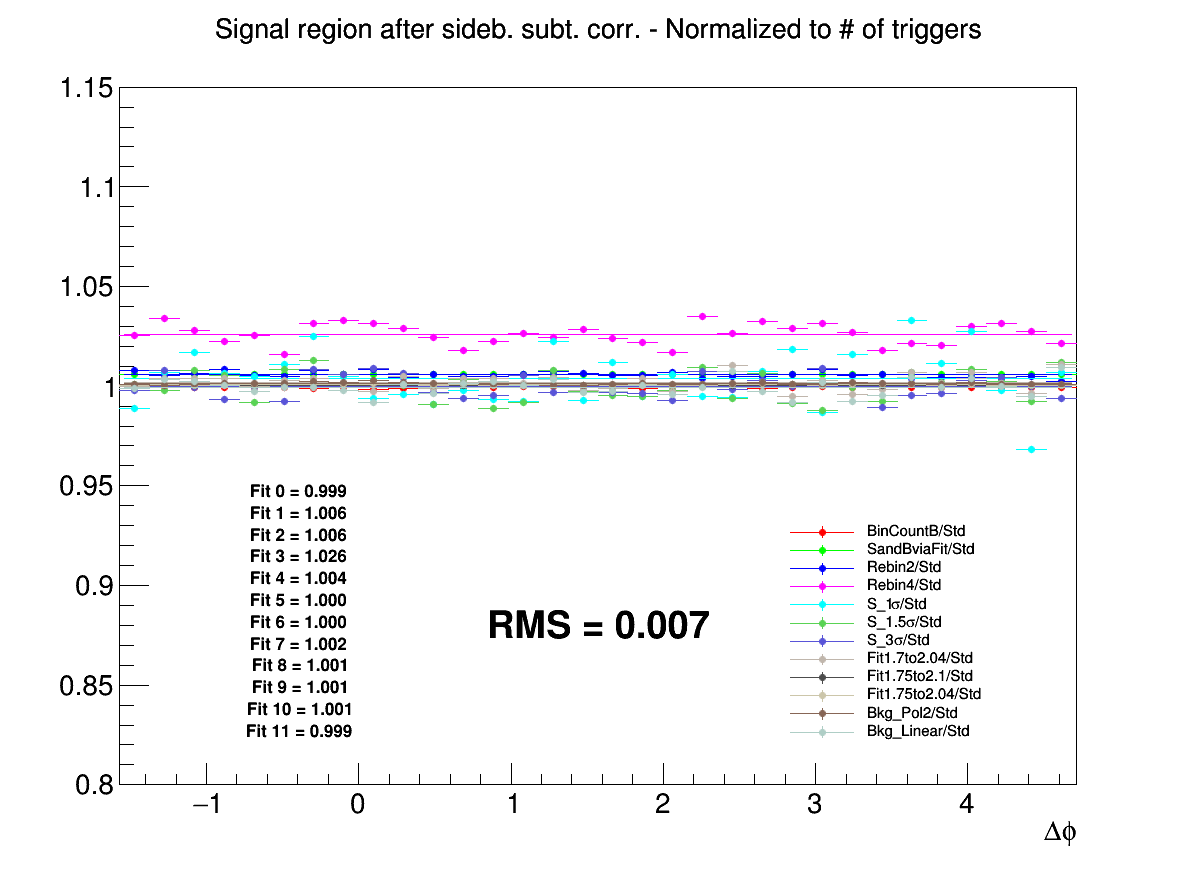
\includegraphics[width=0.31\linewidth]{figuresVsCent/Dzero/SystSandB/0_20/Ratio_AzimCorrDistr_Dzero_Canvas_PtIntBins4to5_PoolInt_thr03to99.png}}
{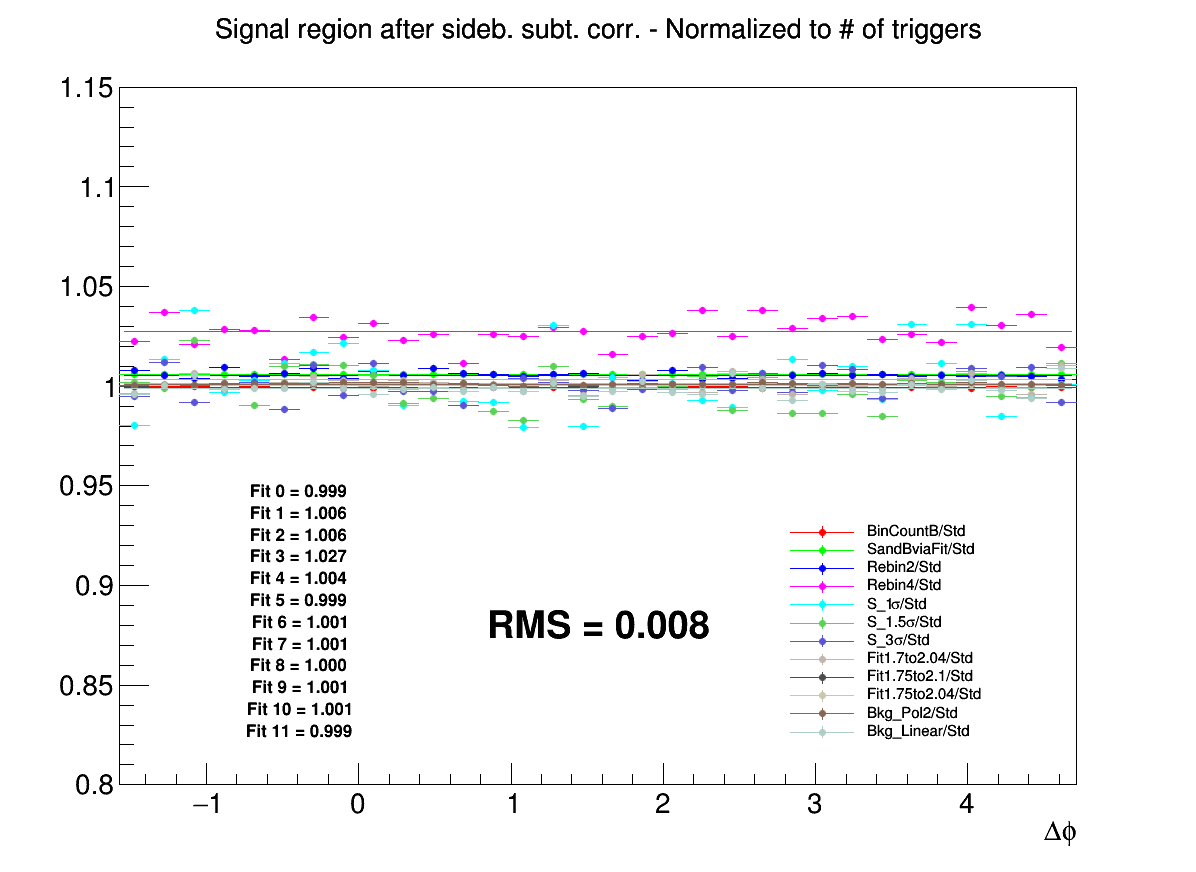
\includegraphics[width=0.31\linewidth]{figuresVsCent/Dzero/SystSandB/0_20/Ratio_AzimCorrDistr_Dzero_Canvas_PtIntBins4to5_PoolInt_thr03to1.png}}
{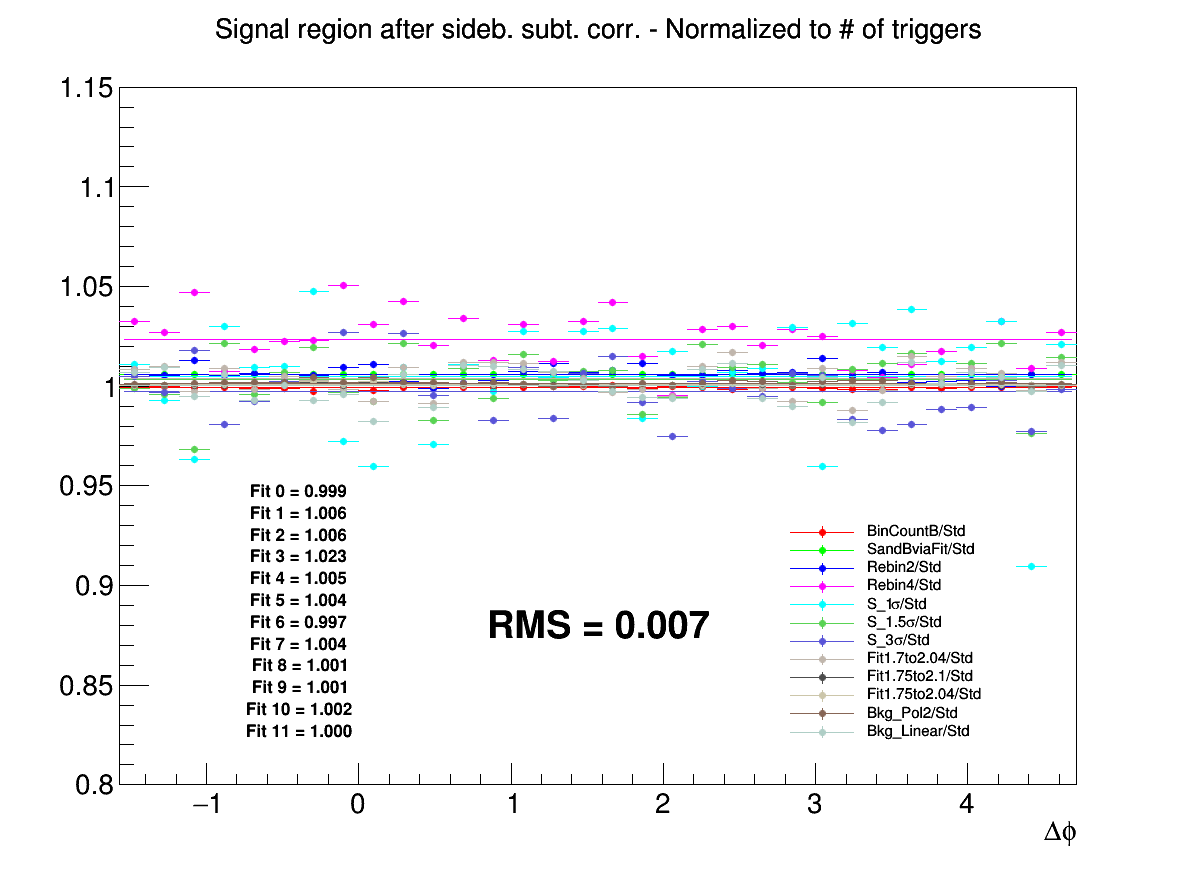
\includegraphics[width=0.31\linewidth]{figuresVsCent/Dzero/SystSandB/0_20/Ratio_AzimCorrDistr_Dzero_Canvas_PtIntBins4to5_PoolInt_thr1to99.png}} \\
{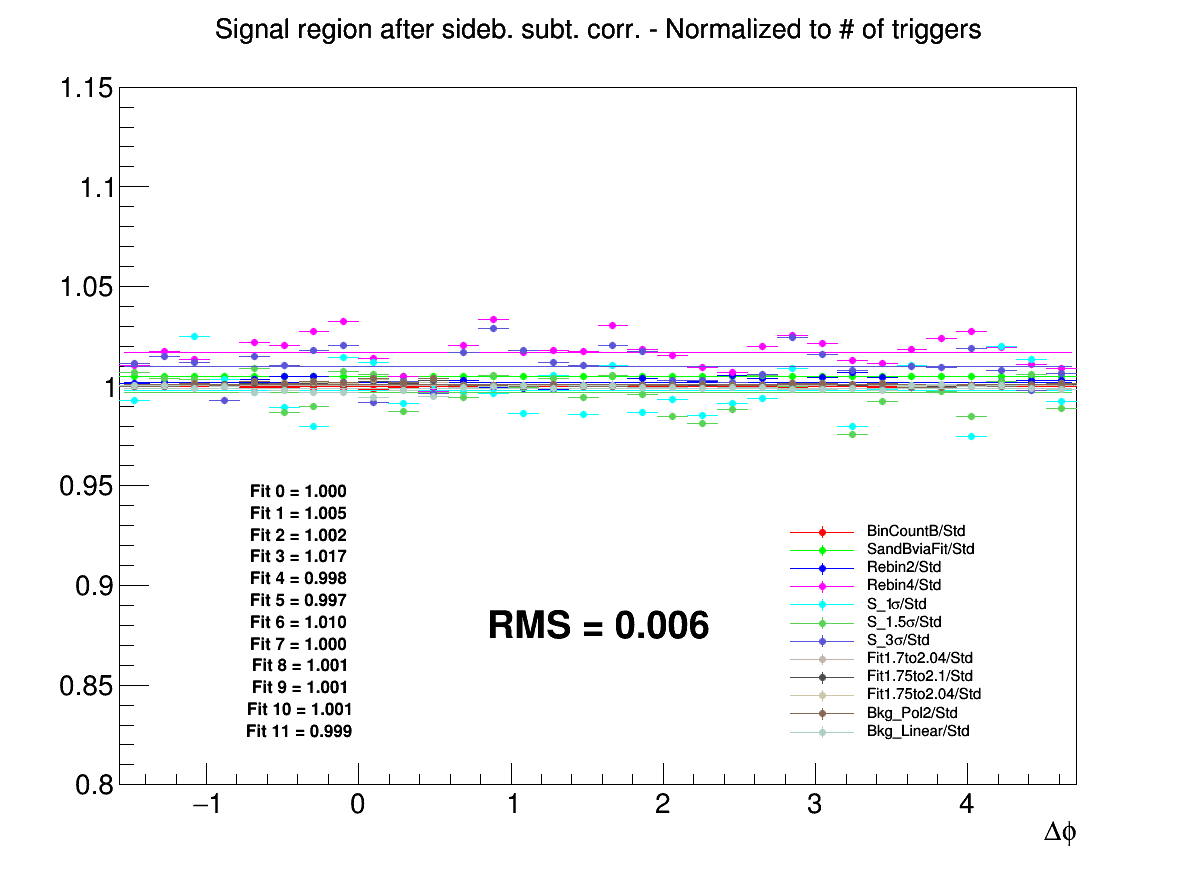
\includegraphics[width=0.31\linewidth]{figuresVsCent/Dzero/SystSandB/0_20/Ratio_AzimCorrDistr_Dzero_Canvas_PtIntBins6to8_PoolInt_thr03to99.png}}
{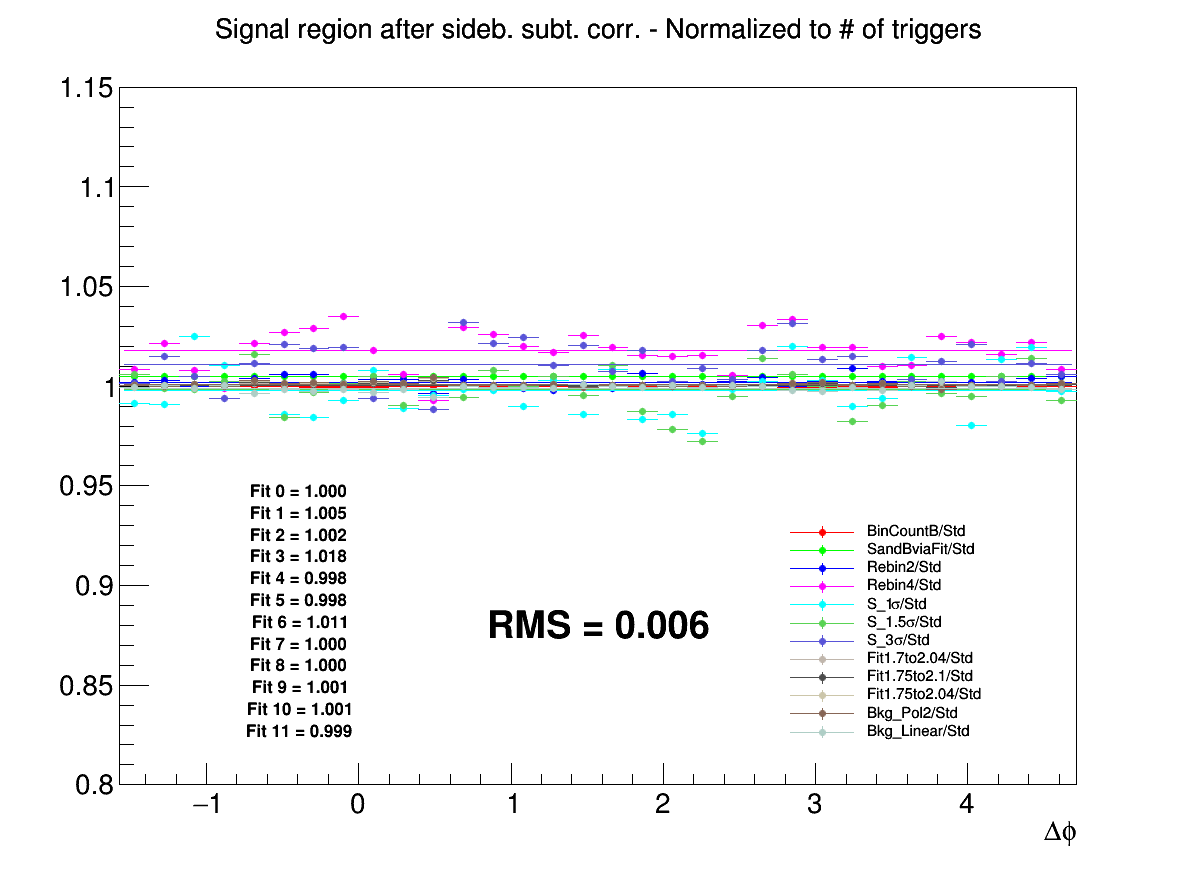
\includegraphics[width=0.31\linewidth]{figuresVsCent/Dzero/SystSandB/0_20/Ratio_AzimCorrDistr_Dzero_Canvas_PtIntBins6to8_PoolInt_thr03to1.png}}
{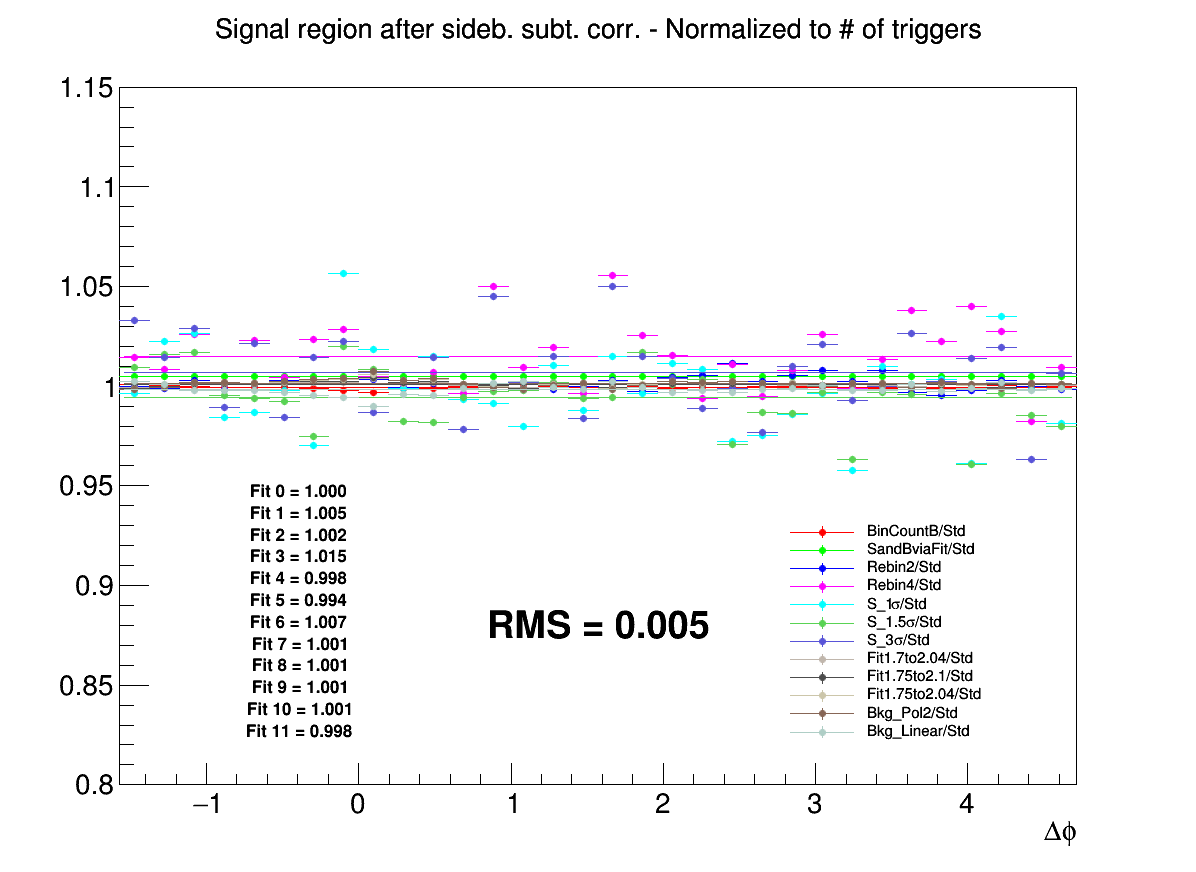
\includegraphics[width=0.31\linewidth]{figuresVsCent/Dzero/SystSandB/0_20/Ratio_AzimCorrDistr_Dzero_Canvas_PtIntBins6to8_PoolInt_thr1to99.png}} \\
{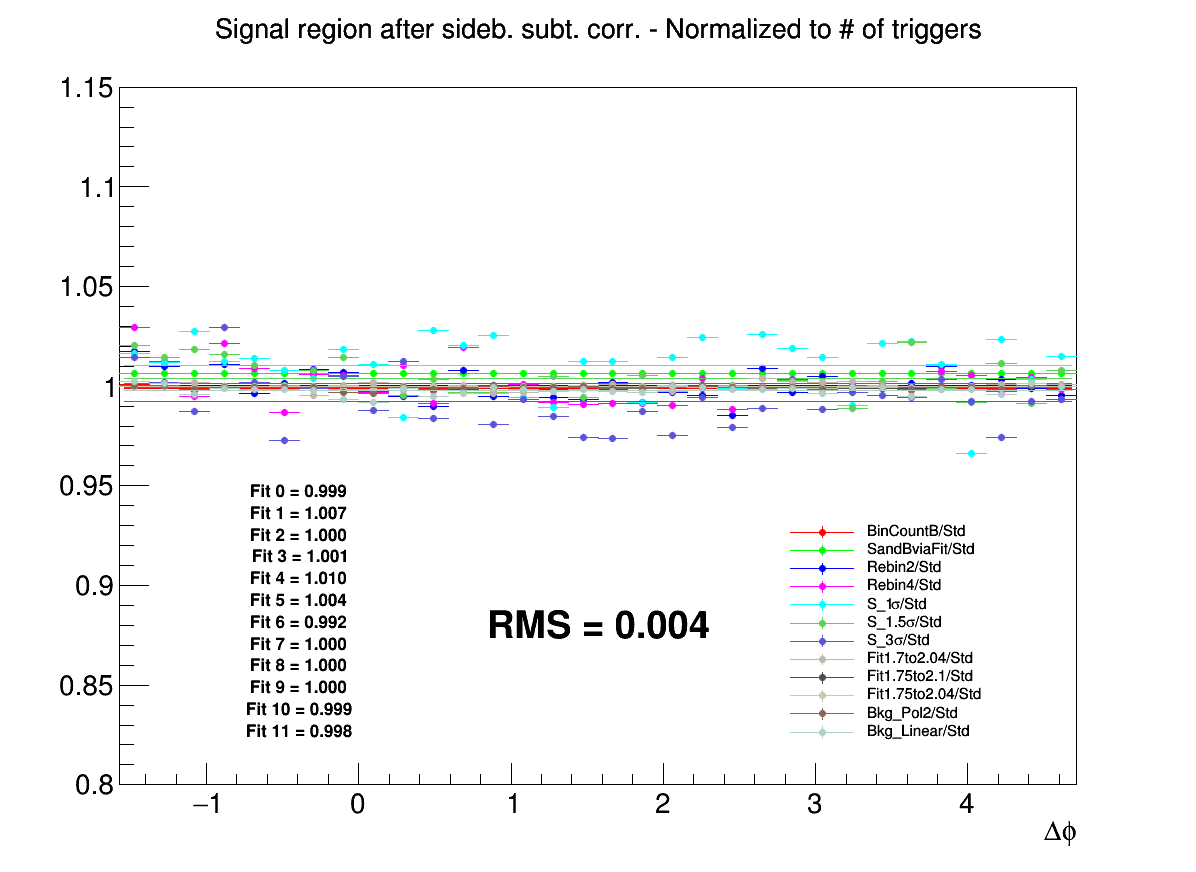
\includegraphics[width=0.31\linewidth]{figuresVsCent/Dzero/SystSandB/0_20/Ratio_AzimCorrDistr_Dzero_Canvas_PtIntBins9to11_PoolInt_thr03to99.png}}
{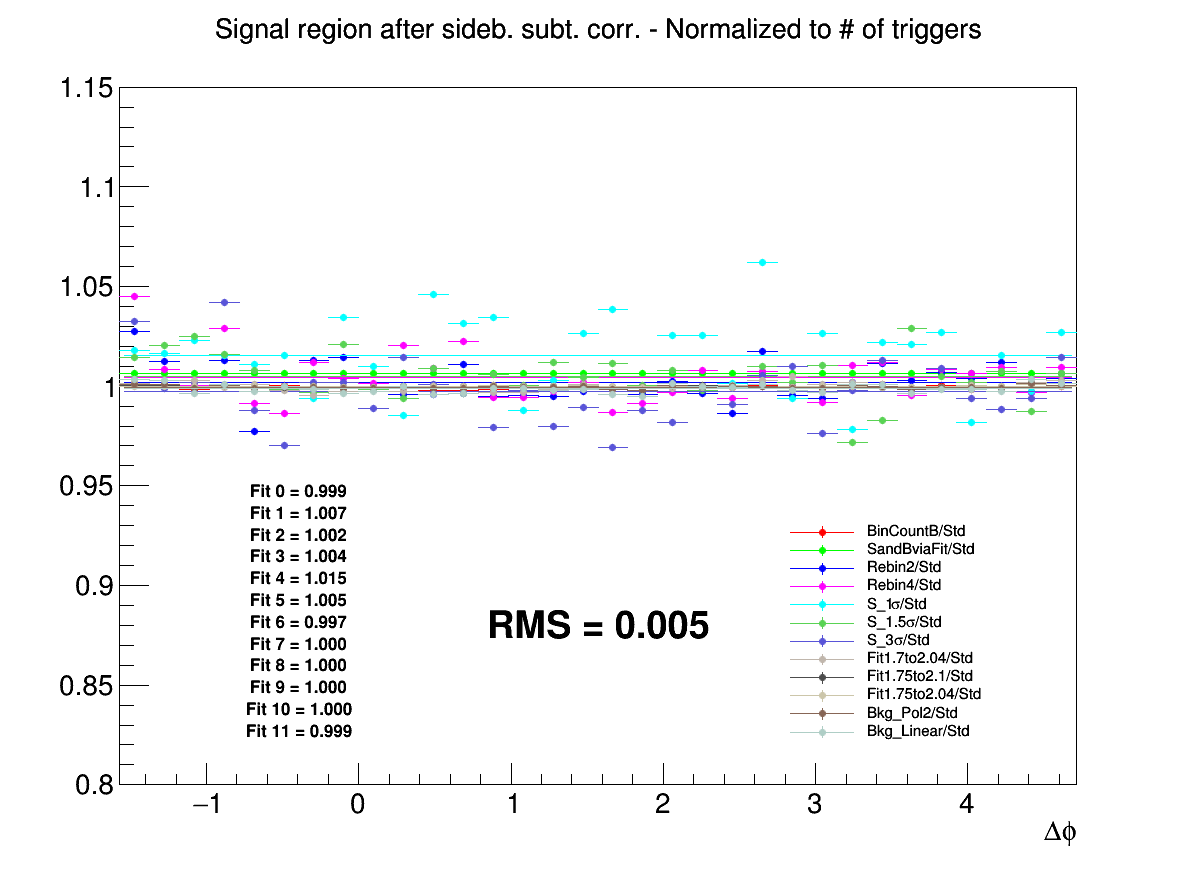
\includegraphics[width=0.31\linewidth]{figuresVsCent/Dzero/SystSandB/0_20/Ratio_AzimCorrDistr_Dzero_Canvas_PtIntBins9to11_PoolInt_thr03to1.png}}
{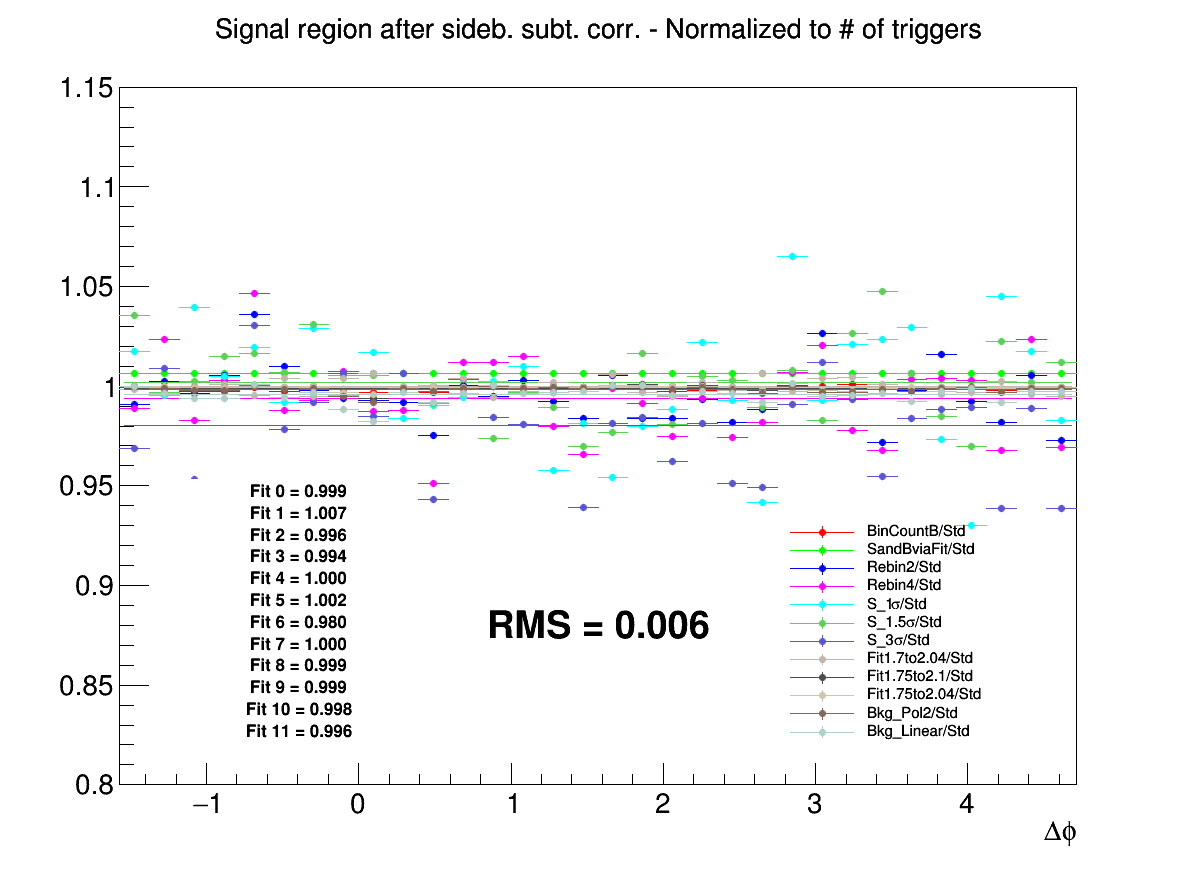
\includegraphics[width=0.31\linewidth]{figuresVsCent/Dzero/SystSandB/0_20/Ratio_AzimCorrDistr_Dzero_Canvas_PtIntBins9to11_PoolInt_thr1to99.png}} \\
{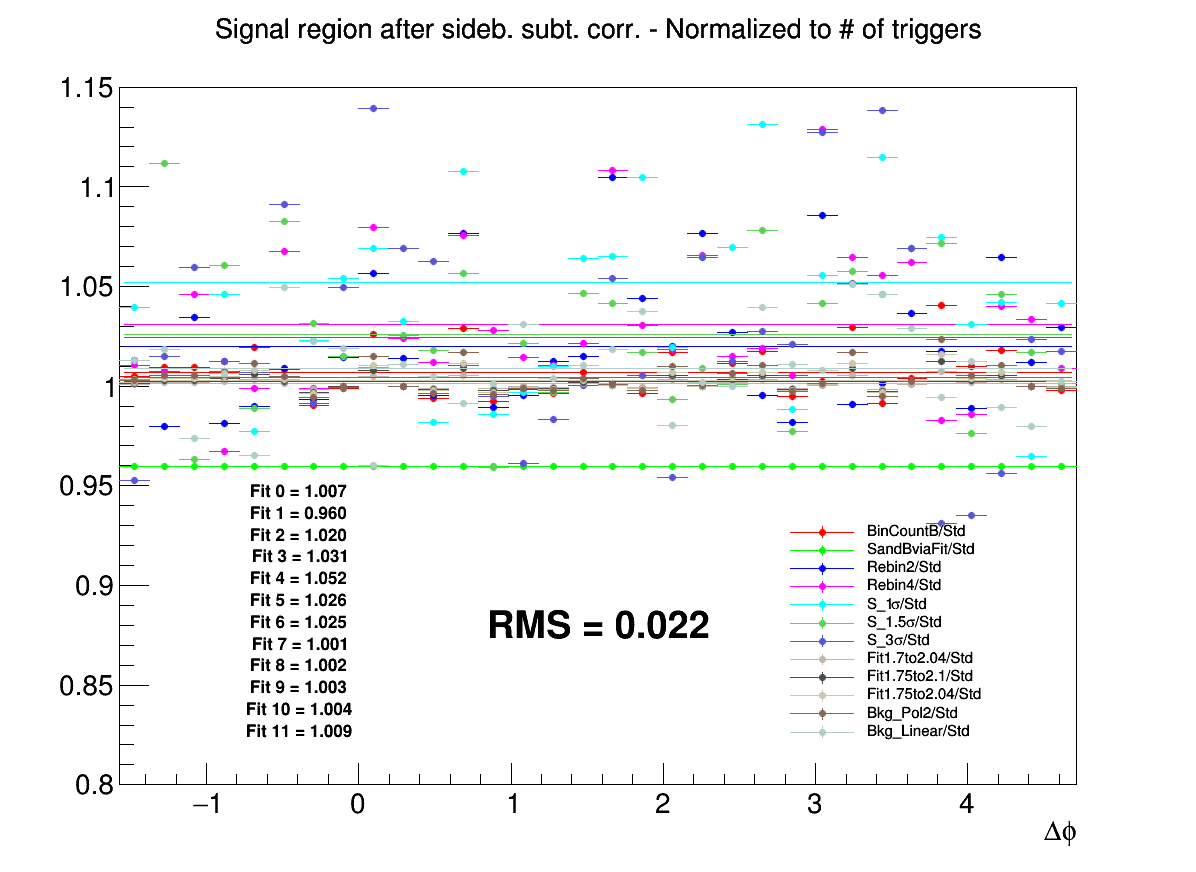
\includegraphics[width=0.31\linewidth]{figuresVsCent/Dzero/SystSandB/0_20/Ratio_AzimCorrDistr_Dzero_Canvas_PtIntBins12to12_PoolInt_thr03to99.png}}
{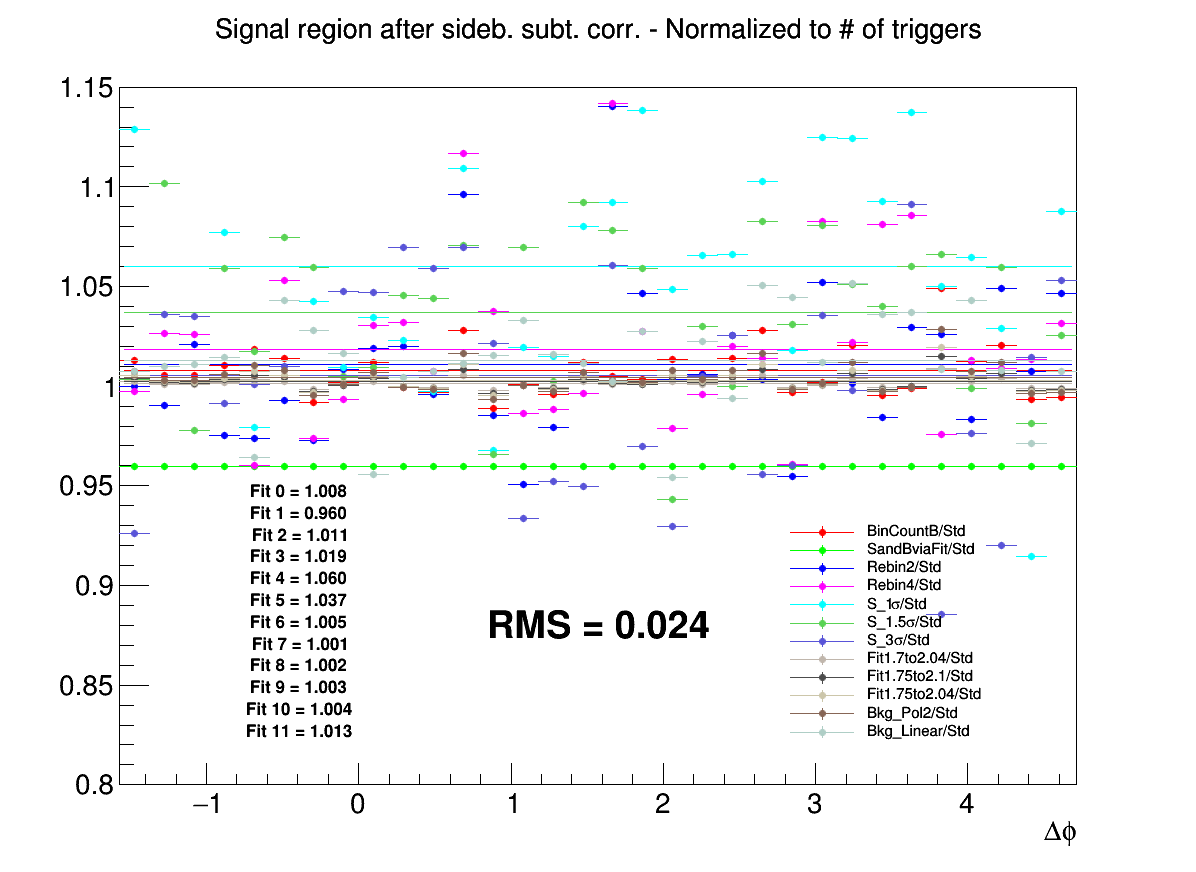
\includegraphics[width=0.31\linewidth]{figuresVsCent/Dzero/SystSandB/0_20/Ratio_AzimCorrDistr_Dzero_Canvas_PtIntBins12to12_PoolInt_thr03to1.png}}
{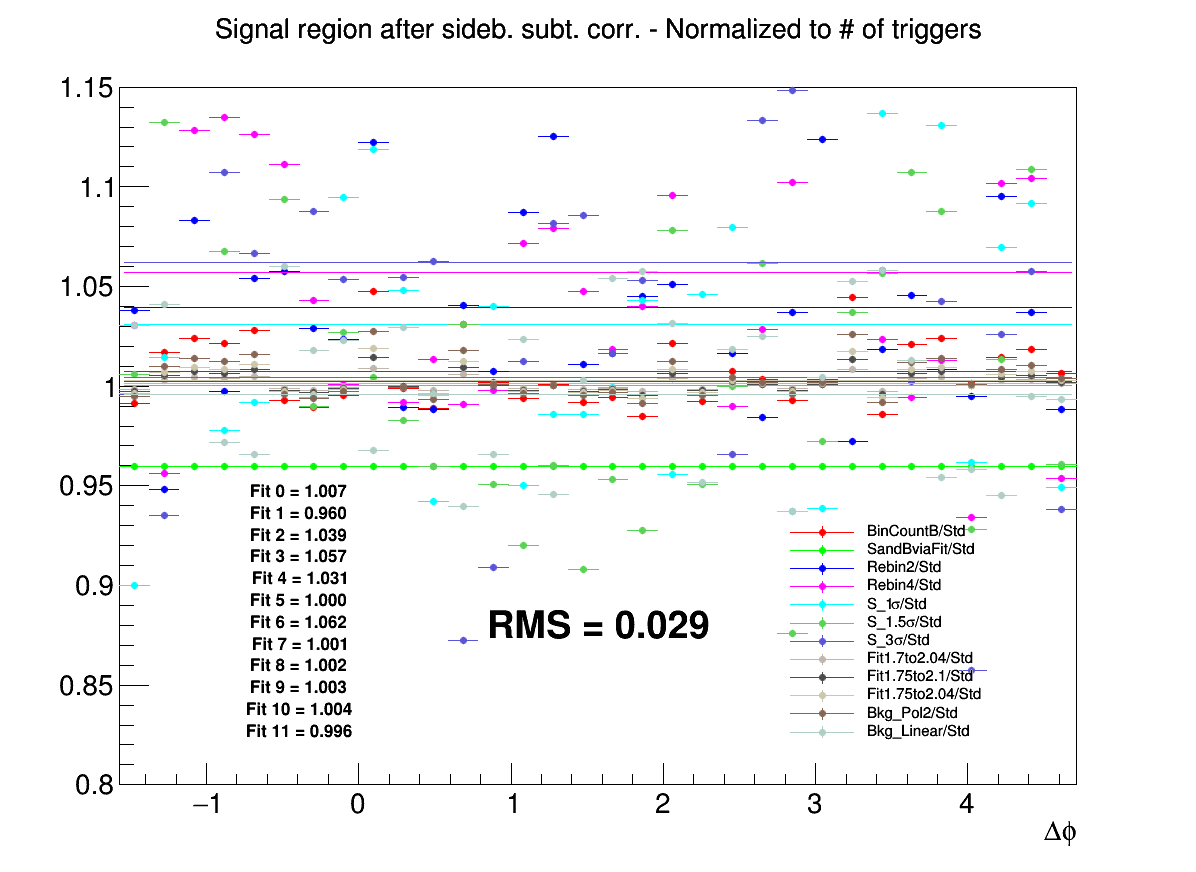
\includegraphics[width=0.31\linewidth]{figuresVsCent/Dzero/SystSandB/0_20/Ratio_AzimCorrDistr_Dzero_Canvas_PtIntBins12to12_PoolInt_thr1to99.png}} \\
 \caption{Ratios of $\Dzero$-h correlation plots obtained with alternate S and B extraction approaches over those obtained with the standard procedure. For 0-20\% centrality. Rows: $\pt$($\Dzero$) 3-5, 5-8, 8-16, 16-24 GeV/$c$. In each row, the panels show the associated track
$\pt$ ranges $> 0.3$, 0.3-1, $> 1$ GeV/$c$, respectively.}
\label{fig:SysSandB020}
\end{figure}

\begin{figure}
\centering
{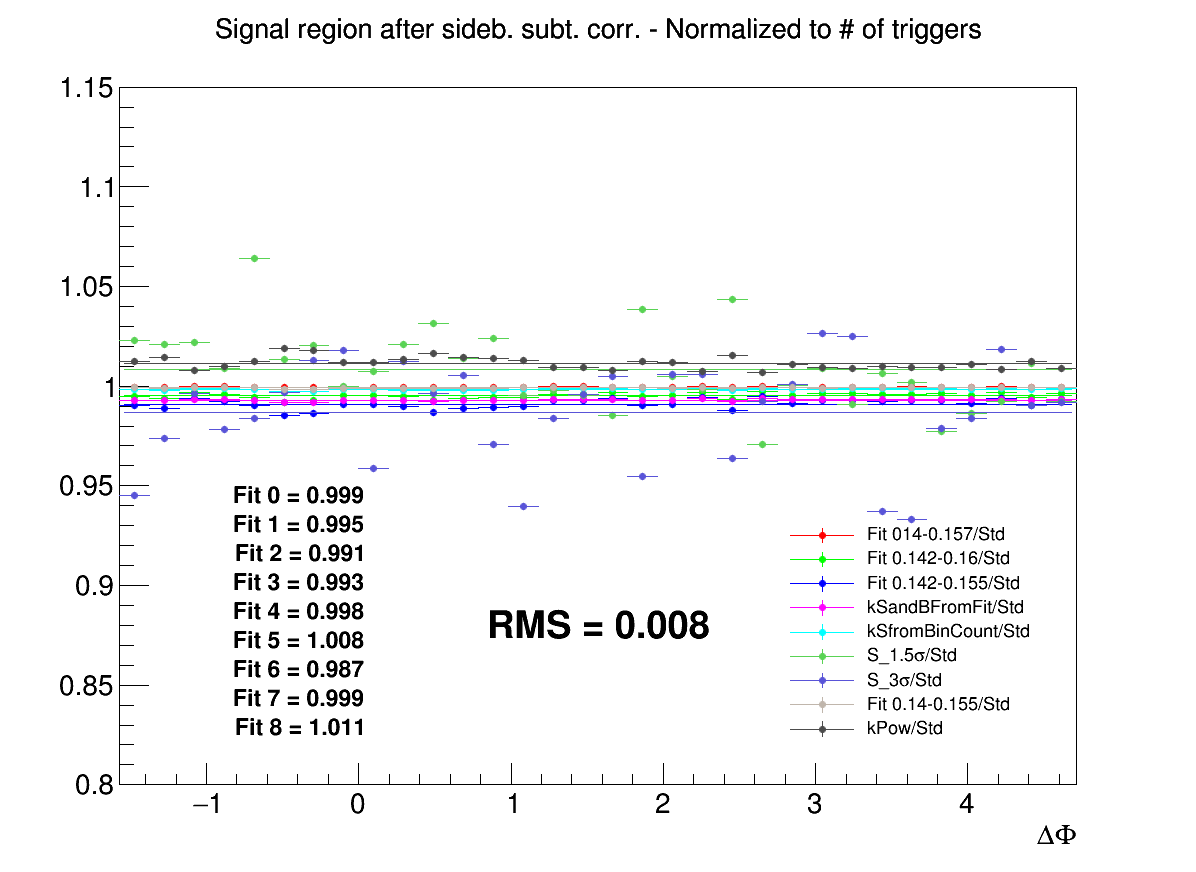
\includegraphics[width=0.31\linewidth]{figuresVsCent/Dstar/SystSandB/020_SandB_Syst/Ratio_AzimCorrDistr_Dstar_Canvas_PtIntBins2to3_PoolInt_thr03to99_YIELD_020.png}}
{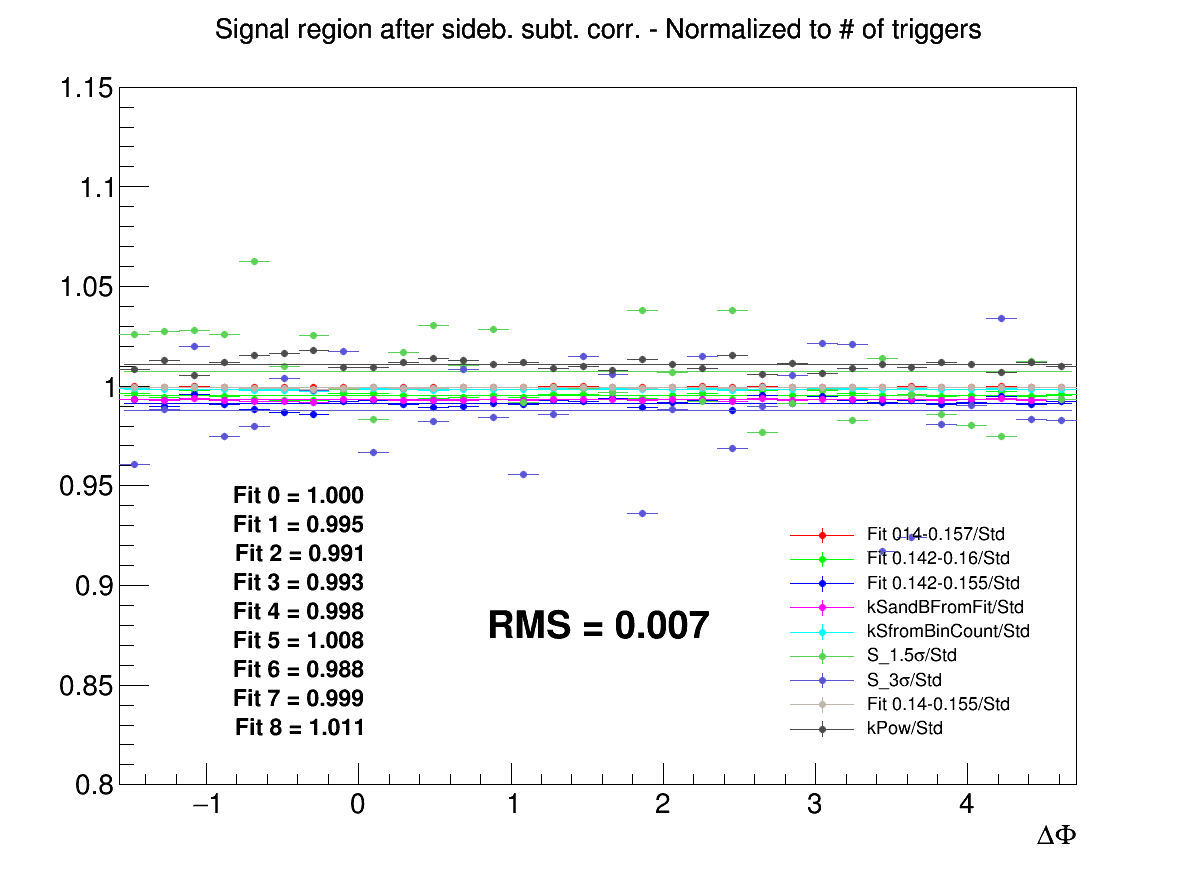
\includegraphics[width=0.31\linewidth]{figuresVsCent/Dstar/SystSandB/020_SandB_Syst/Ratio_AzimCorrDistr_Dstar_Canvas_PtIntBins2to3_PoolInt_thr03to1_YIELD_020.png}}
{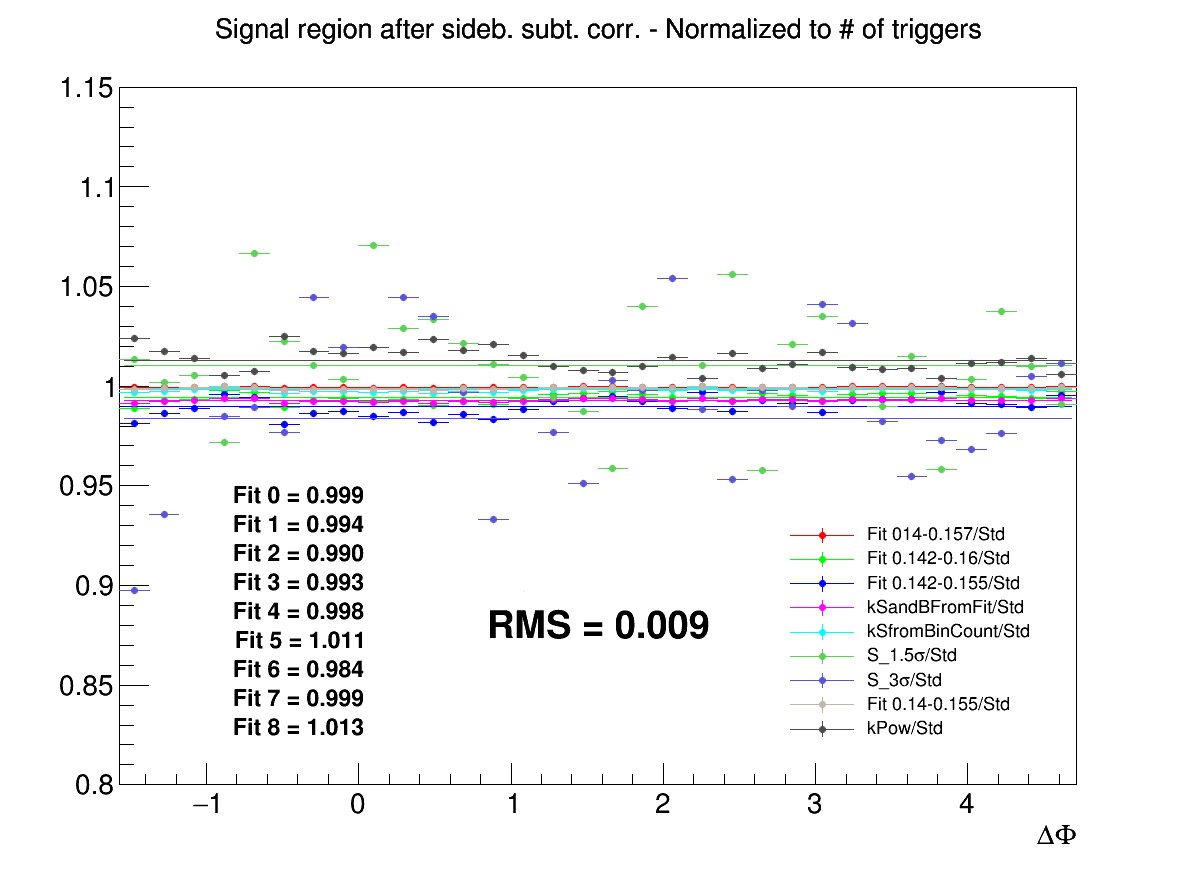
\includegraphics[width=0.31\linewidth]{figuresVsCent/Dstar/SystSandB/020_SandB_Syst/Ratio_AzimCorrDistr_Dstar_Canvas_PtIntBins2to3_PoolInt_thr1to99_YIELD_020.png}} \\

{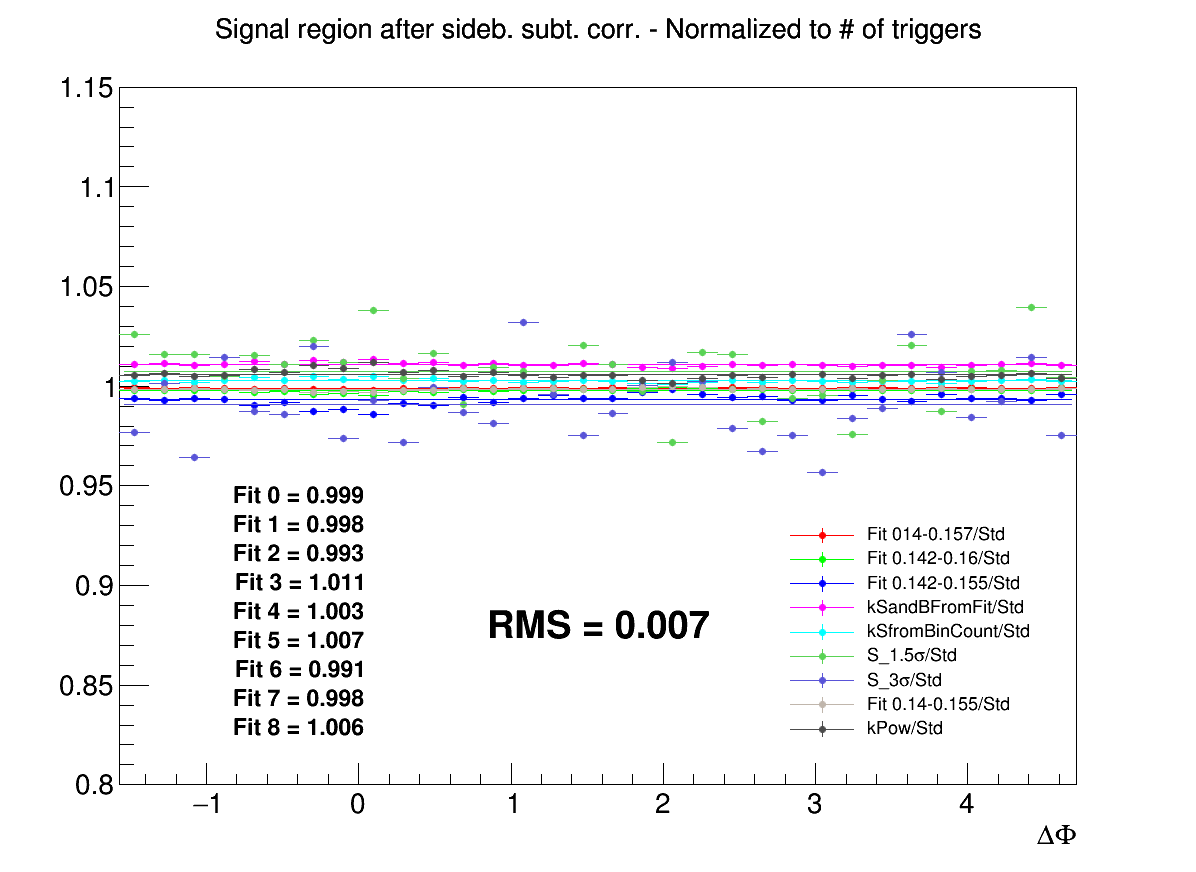
\includegraphics[width=0.31\linewidth]{figuresVsCent/Dstar/SystSandB/020_SandB_Syst/Ratio_AzimCorrDistr_Dstar_Canvas_PtIntBins4to6_PoolInt_thr03to99_YIELD_020.png}}
{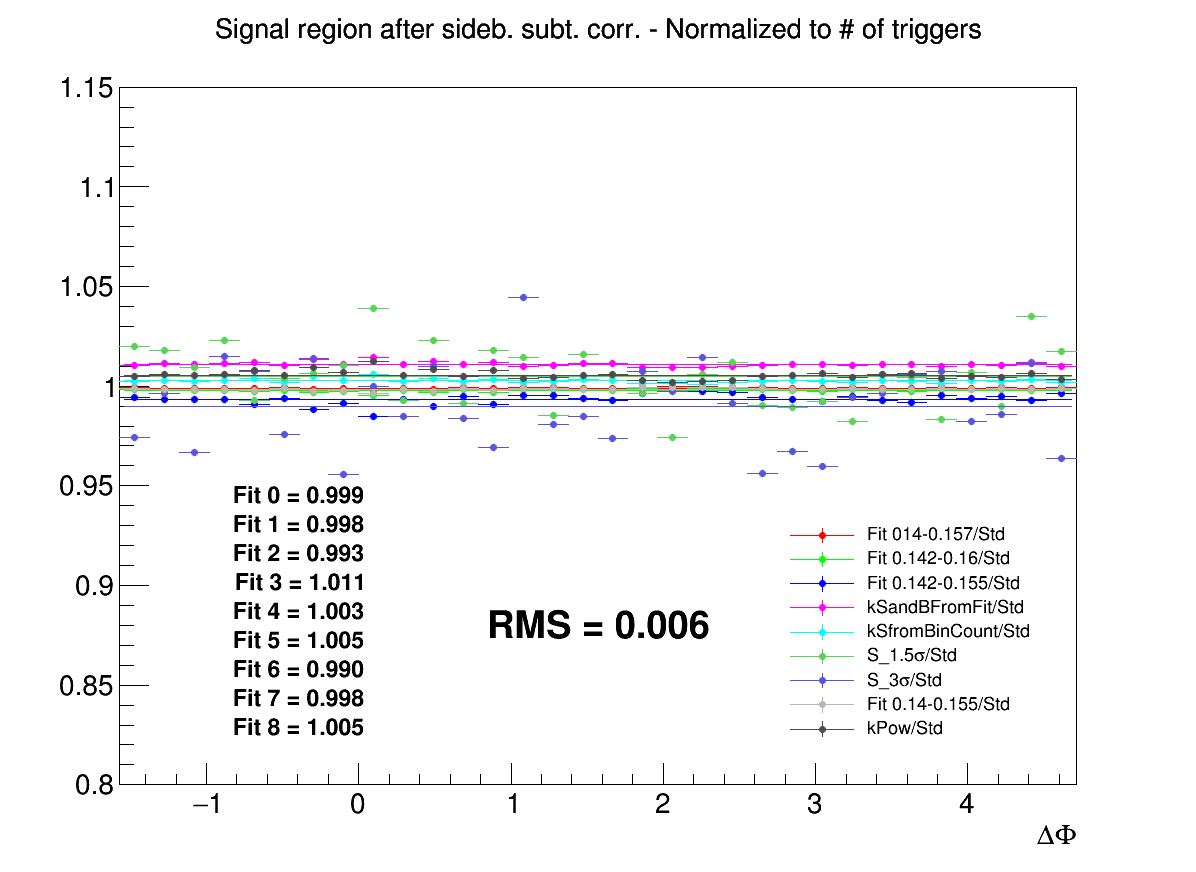
\includegraphics[width=0.31\linewidth]{figuresVsCent/Dstar/SystSandB/020_SandB_Syst/Ratio_AzimCorrDistr_Dstar_Canvas_PtIntBins4to6_PoolInt_thr03to1_YIELD_020.png}}
{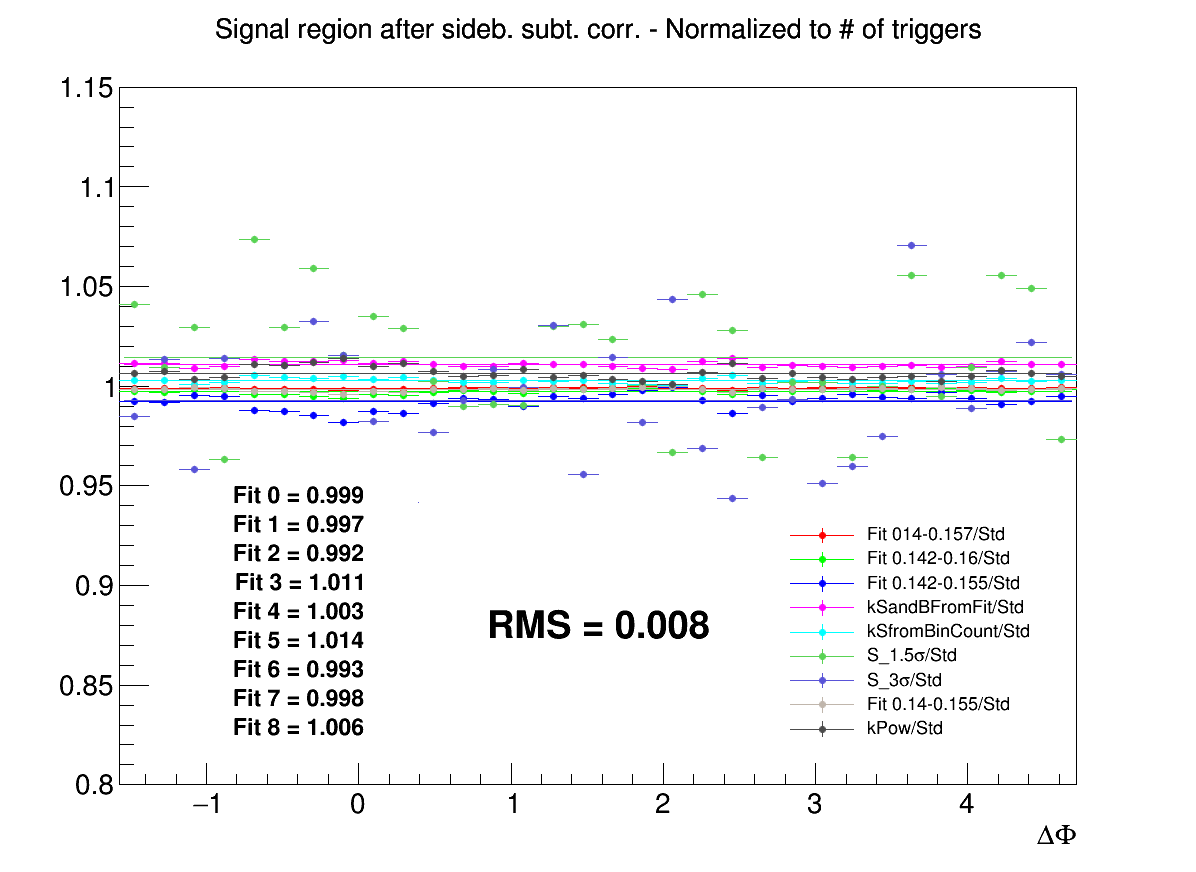
\includegraphics[width=0.31\linewidth]{figuresVsCent/Dstar/SystSandB/020_SandB_Syst/Ratio_AzimCorrDistr_Dstar_Canvas_PtIntBins4to6_PoolInt_thr1to99_YIELD_020.png}} \\

{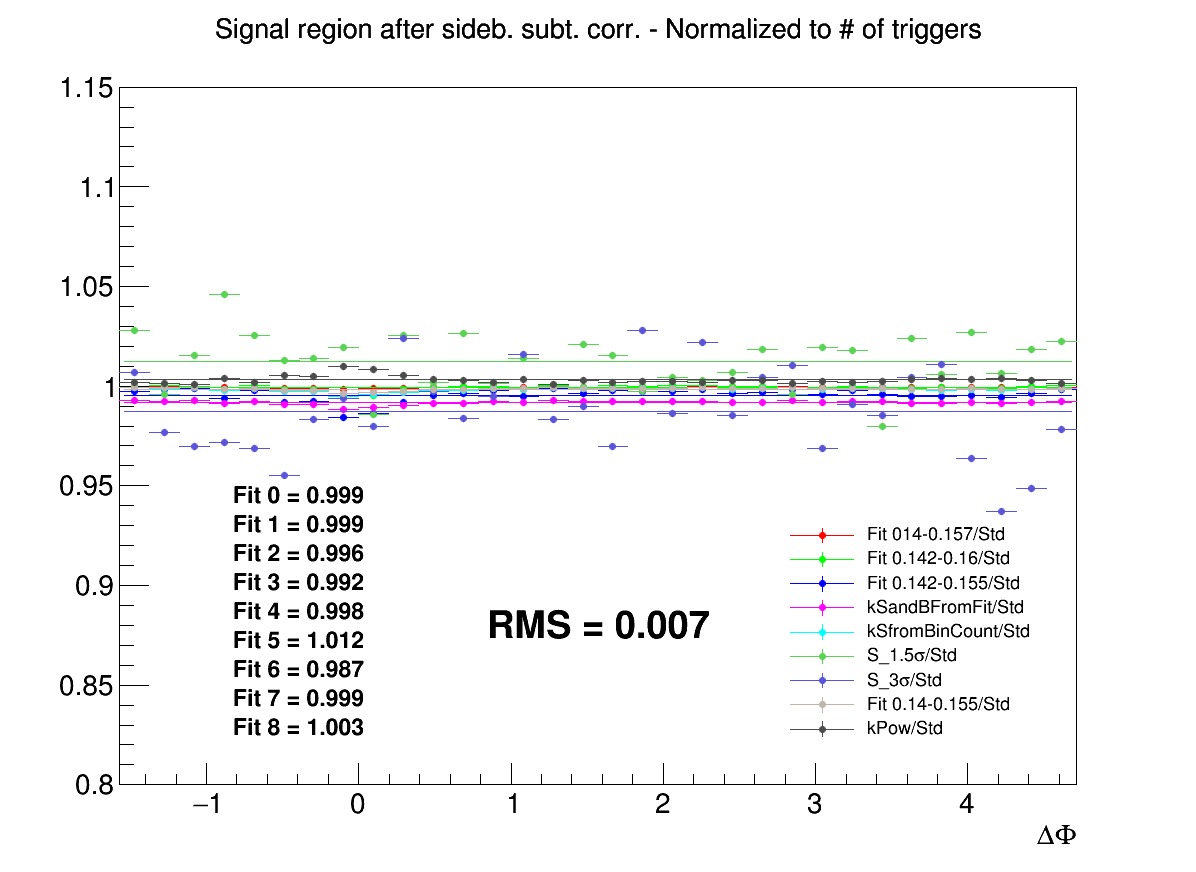
\includegraphics[width=0.31\linewidth]{figuresVsCent/Dstar/SystSandB/020_SandB_Syst/Ratio_AzimCorrDistr_Dstar_Canvas_PtIntBins7to9_PoolInt_thr03to99_YIELD_020.png}}
{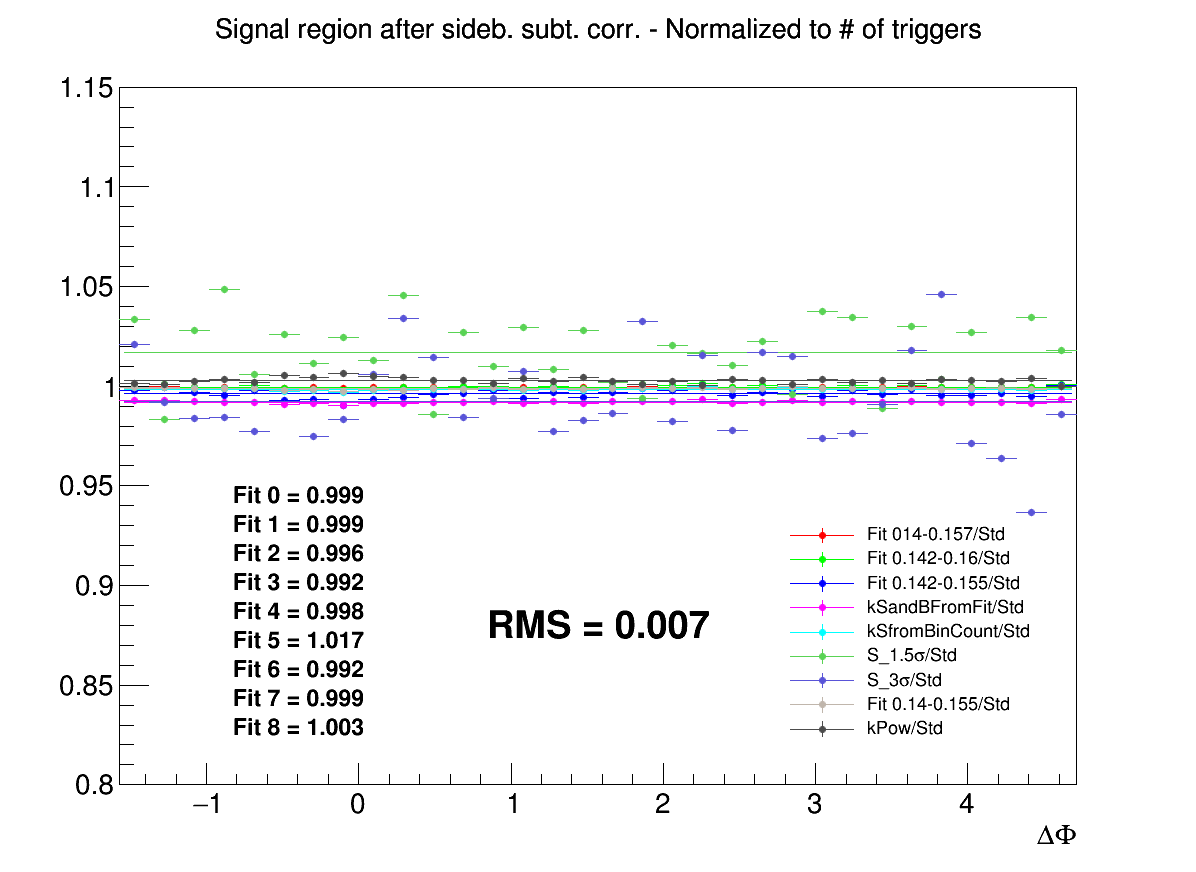
\includegraphics[width=0.31\linewidth]{figuresVsCent/Dstar/SystSandB/020_SandB_Syst/Ratio_AzimCorrDistr_Dstar_Canvas_PtIntBins7to9_PoolInt_thr03to1_YIELD_020.png}}
{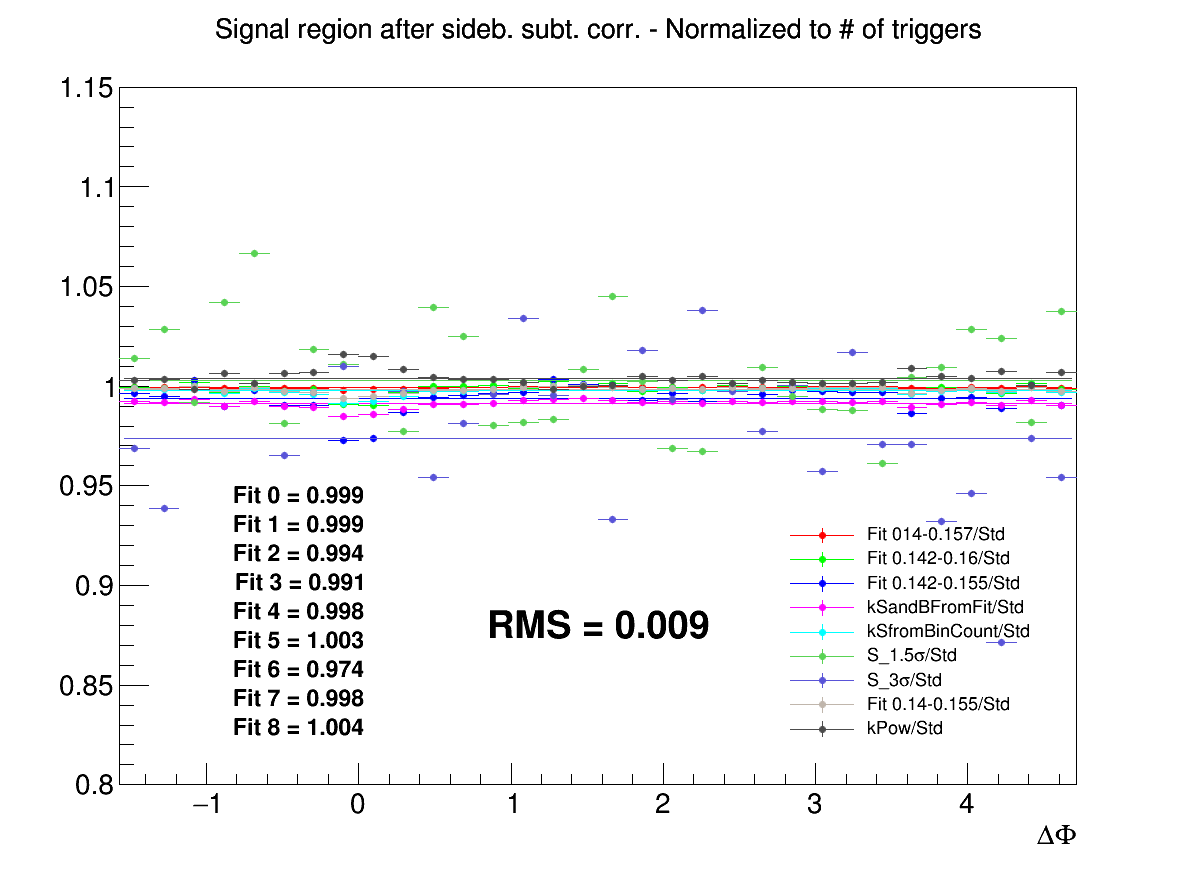
\includegraphics[width=0.31\linewidth]{figuresVsCent/Dstar/SystSandB/020_SandB_Syst/Ratio_AzimCorrDistr_Dstar_Canvas_PtIntBins7to9_PoolInt_thr1to99_YIELD_020.png}} \\

{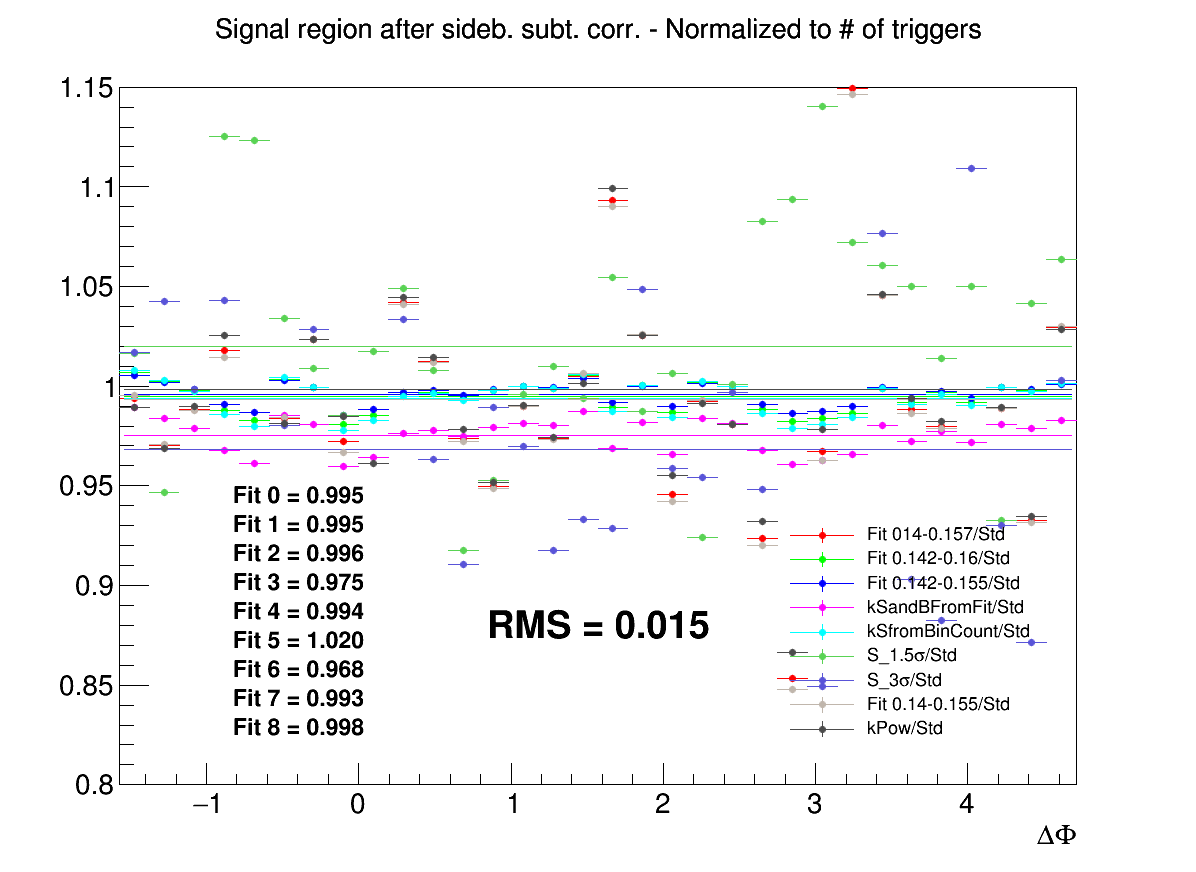
\includegraphics[width=0.31\linewidth]{figuresVsCent/Dstar/SystSandB/020_SandB_Syst/Ratio_AzimCorrDistr_Dstar_Canvas_PtIntBins10to10_PoolInt_thr03to99_YIELD_020.png}}
{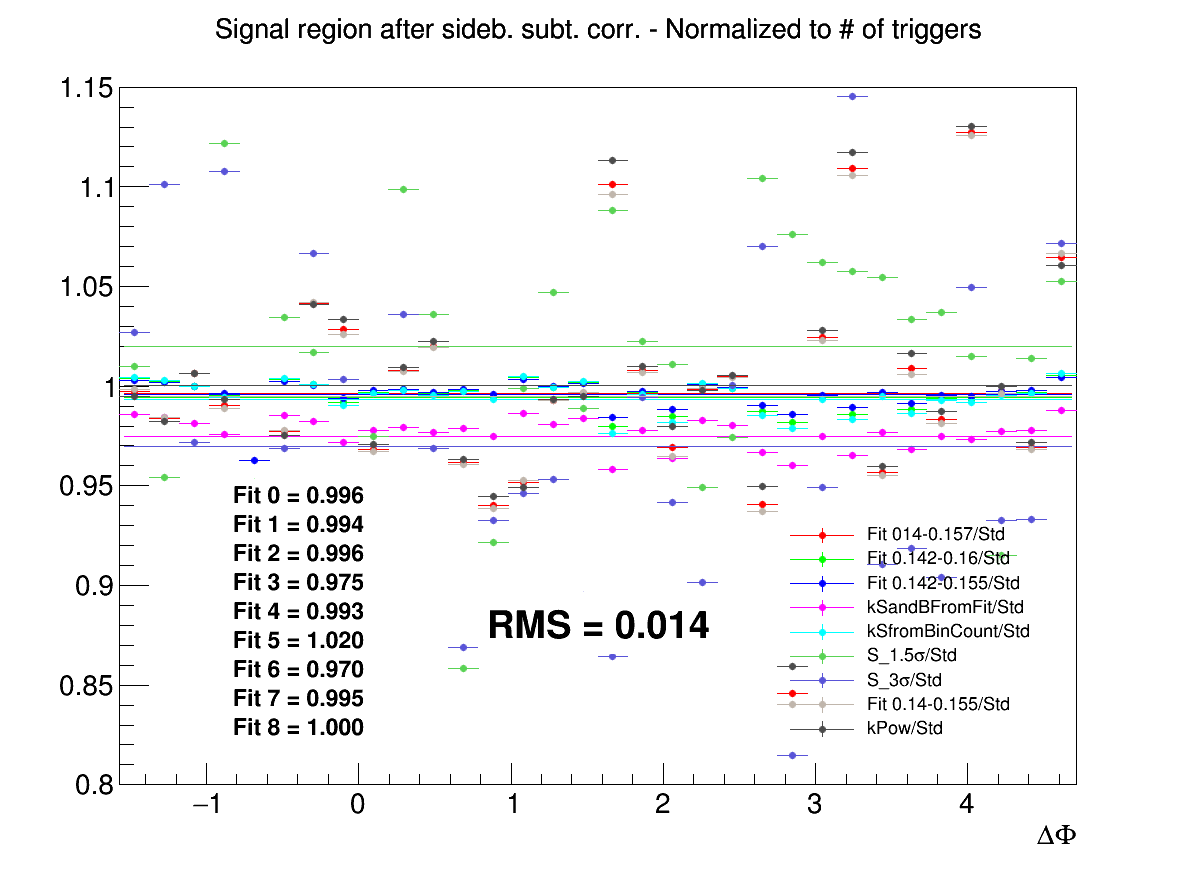
\includegraphics[width=0.31\linewidth]{figuresVsCent/Dstar/SystSandB/020_SandB_Syst/Ratio_AzimCorrDistr_Dstar_Canvas_PtIntBins10to10_PoolInt_thr03to1_YIELD_020.png}}
{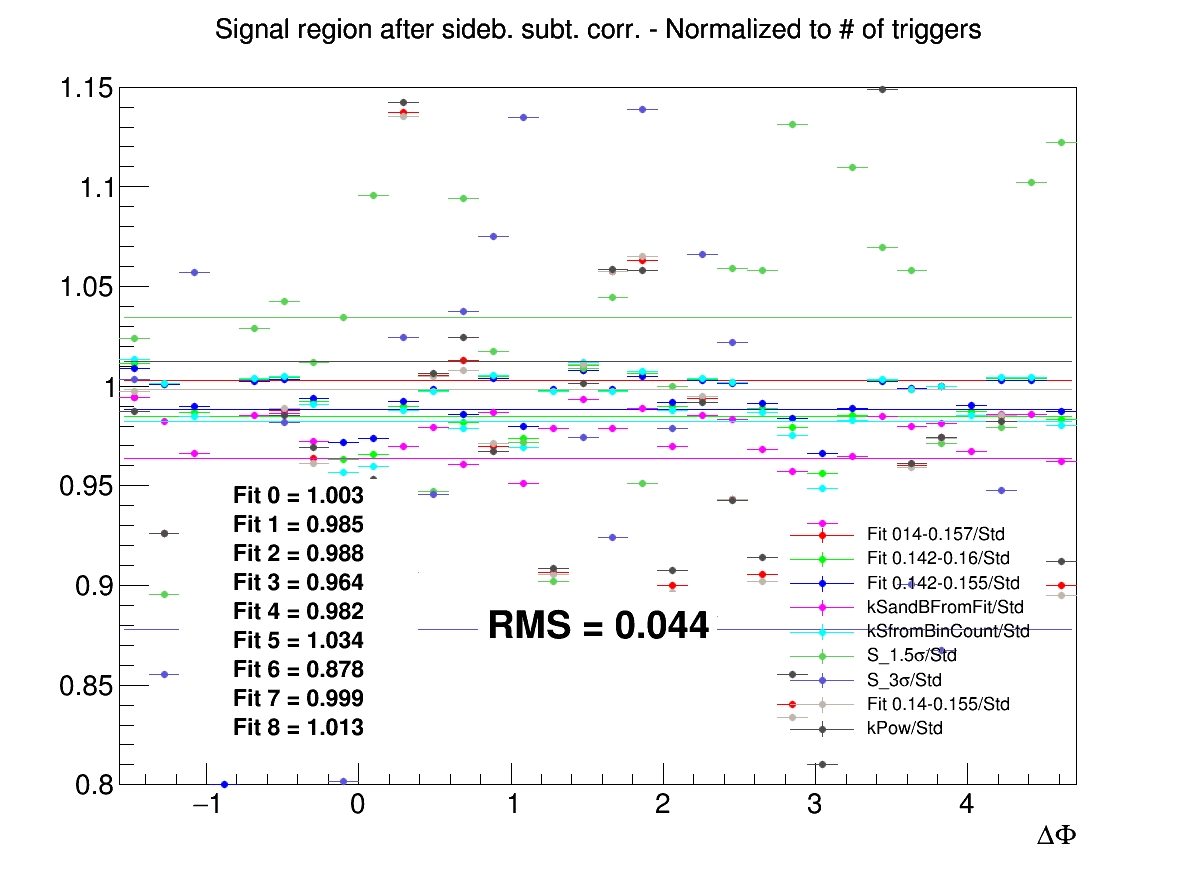
\includegraphics[width=0.31\linewidth]{figuresVsCent/Dstar/SystSandB/020_SandB_Syst/Ratio_AzimCorrDistr_Dstar_Canvas_PtIntBins10to10_PoolInt_thr1to99_YIELD_020.png}} \\
 \caption{Ratios of $\Dstar$-h correlation plots obtained with alternate S and B extraction approaches over those obtained with the standard procedure. For 0-20\% centrality. Rows: $\pt$($\Dstar$) 3-5, 5-8, 8-16, 16-24 GeV/$c$. In each row, the panels show the associated track
$\pt$ ranges $> 0.3$, 0.3-1, $> 1$ GeV/$c$, respectively.}
\label{fig:SysSandB020Dstar}
\end{figure}


% 0_20% Dplus Systematics
\begin{figure}
\centering
{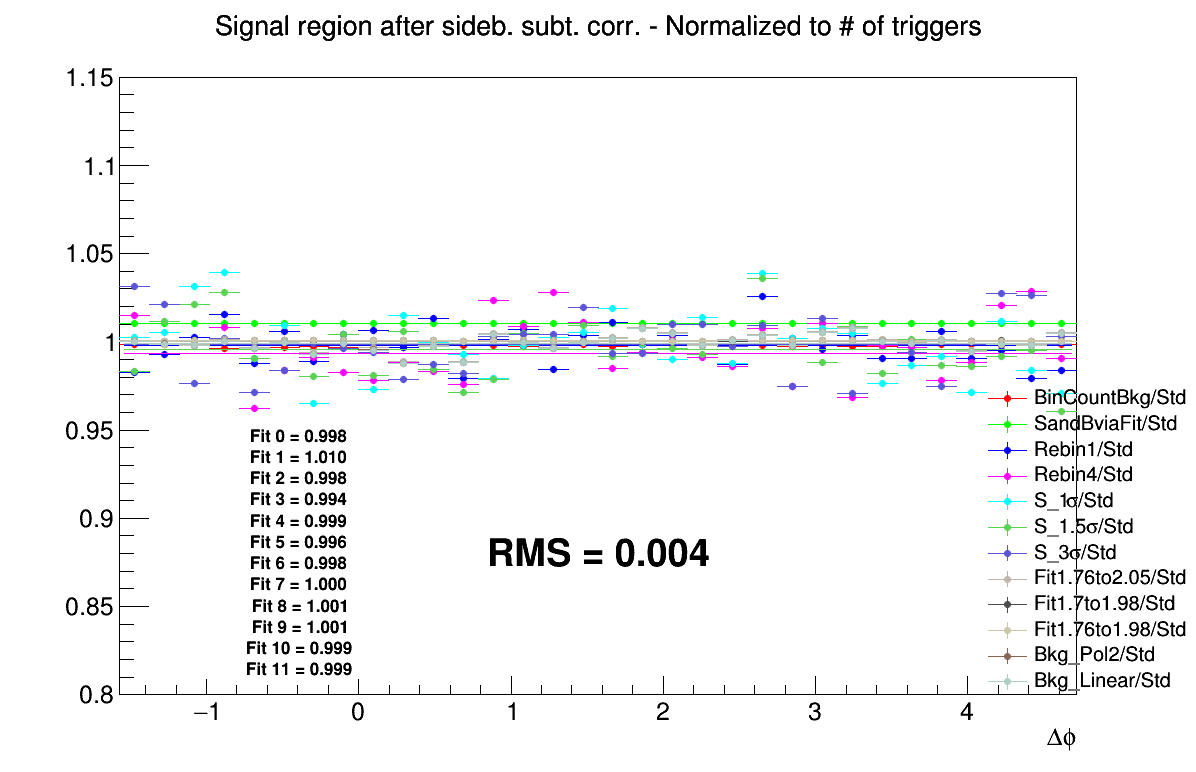
\includegraphics[width=0.31\linewidth]{Centrality_DPlus/Dplus/Systematic/0_20/Yield/Ratio_AzimCorrDistr_Dplus_Canvas_PtIntBins3to4_PoolInt_thrdot3to99dot.png}}
{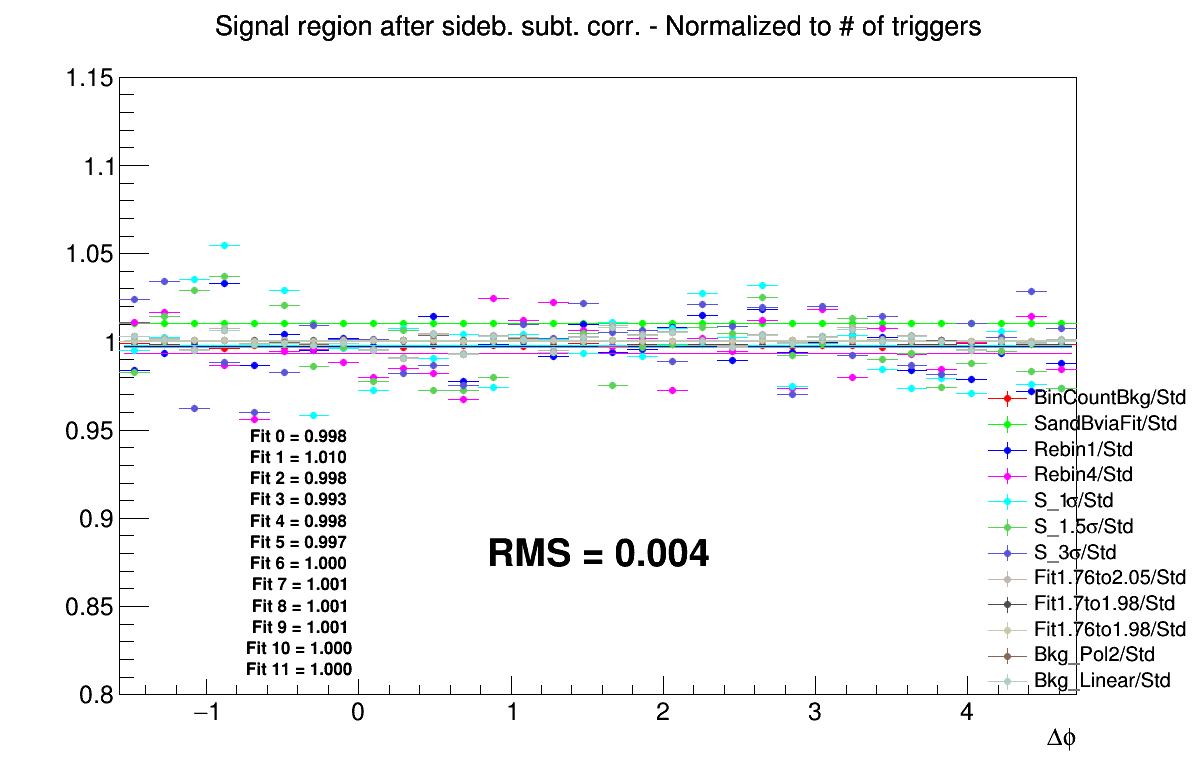
\includegraphics[width=0.31\linewidth]{Centrality_DPlus/Dplus/Systematic/0_20/Yield/Ratio_AzimCorrDistr_Dplus_Canvas_PtIntBins3to4_PoolInt_thrdot3to1dot.png}}
{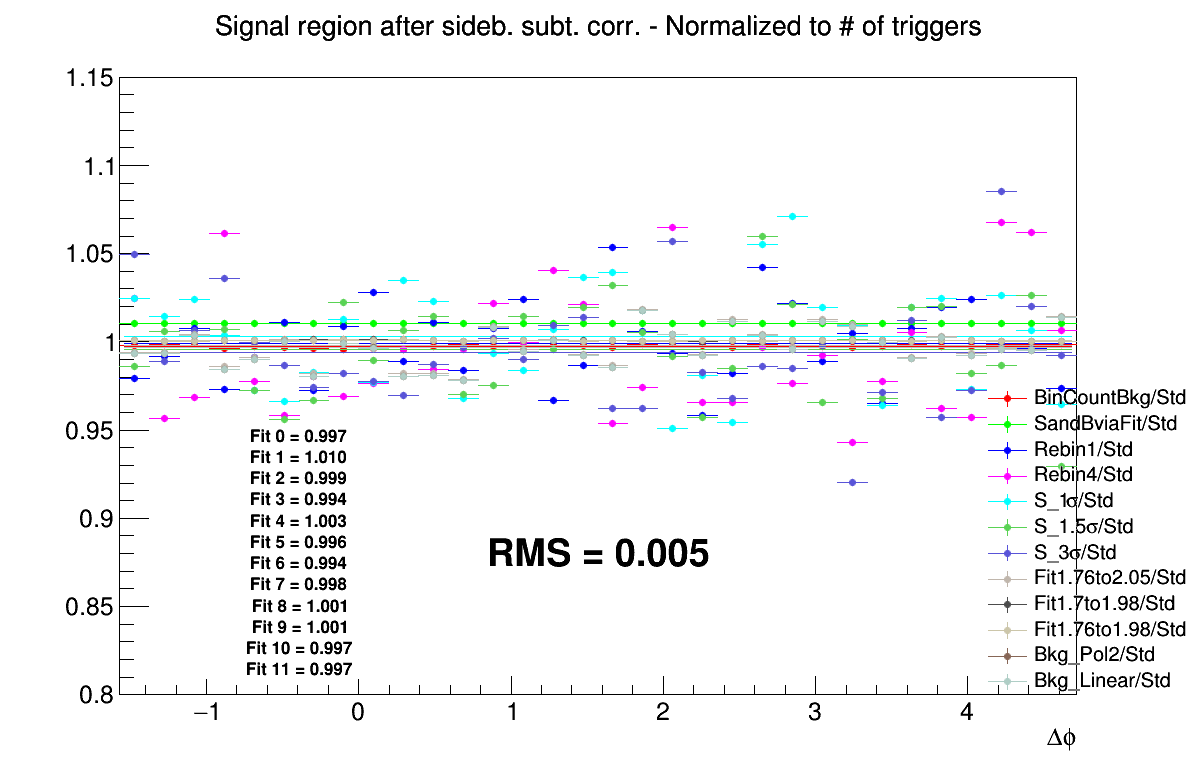
\includegraphics[width=0.31\linewidth]{Centrality_DPlus/Dplus/Systematic/0_20/Yield/Ratio_AzimCorrDistr_Dplus_Canvas_PtIntBins3to4_PoolInt_thr1dotto99dot.png}} \\
{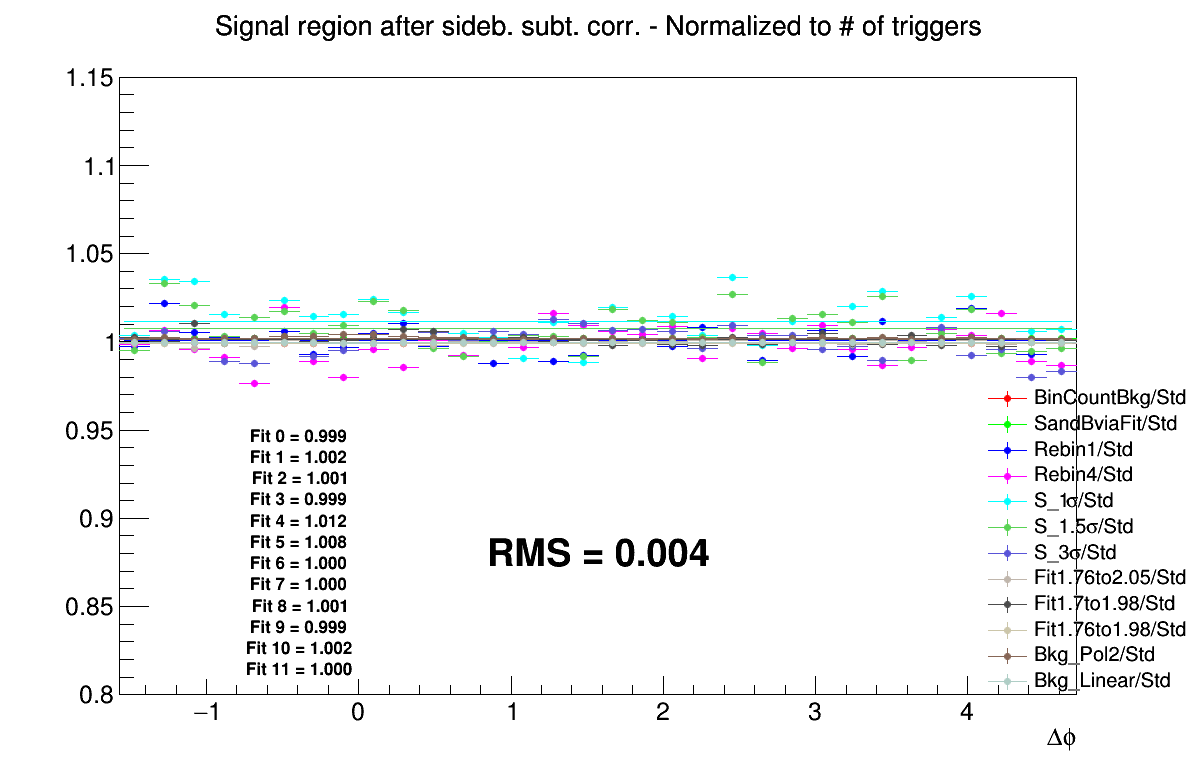
\includegraphics[width=0.31\linewidth]{Centrality_DPlus/Dplus/Systematic/0_20/Yield/Ratio_AzimCorrDistr_Dplus_Canvas_PtIntBins5to7_PoolInt_thrdot3to99dot.png}}
{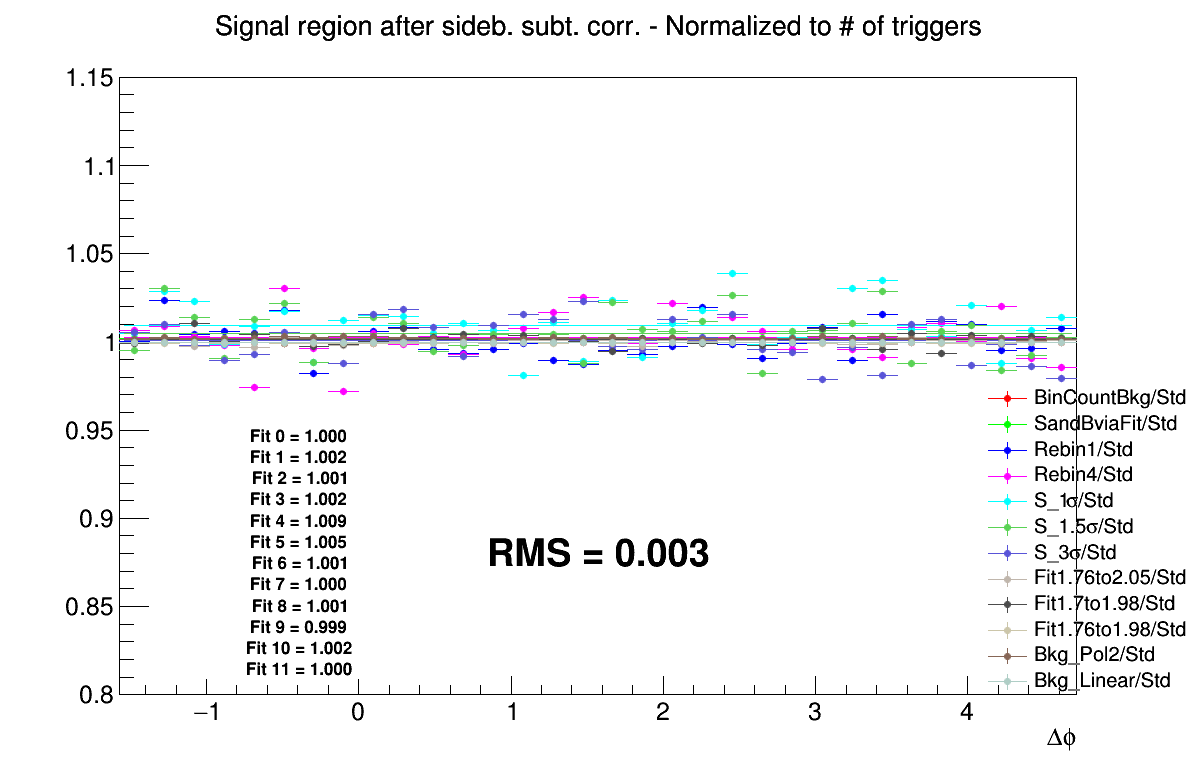
\includegraphics[width=0.31\linewidth]{Centrality_DPlus/Dplus/Systematic/0_20/Yield/Ratio_AzimCorrDistr_Dplus_Canvas_PtIntBins5to7_PoolInt_thrdot3to1dot.png}}
{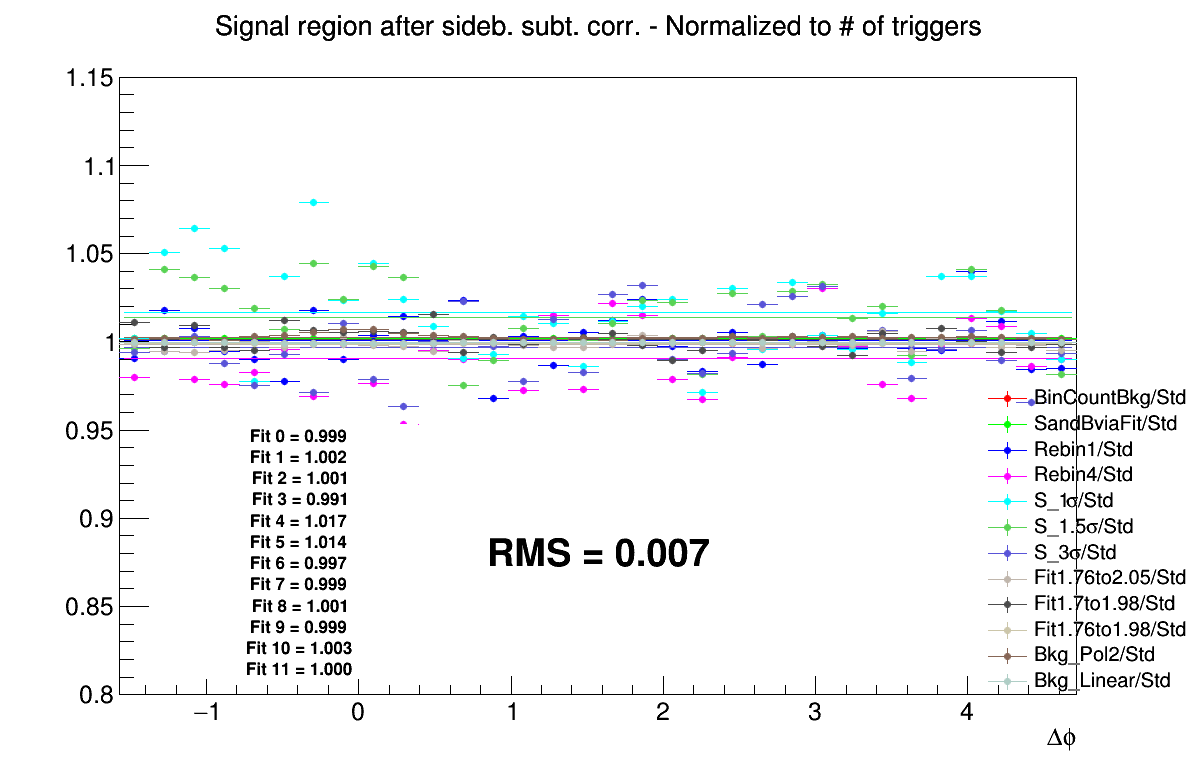
\includegraphics[width=0.31\linewidth]{Centrality_DPlus/Dplus/Systematic/0_20/Yield/Ratio_AzimCorrDistr_Dplus_Canvas_PtIntBins5to7_PoolInt_thr1dotto99dot.png}} \\
{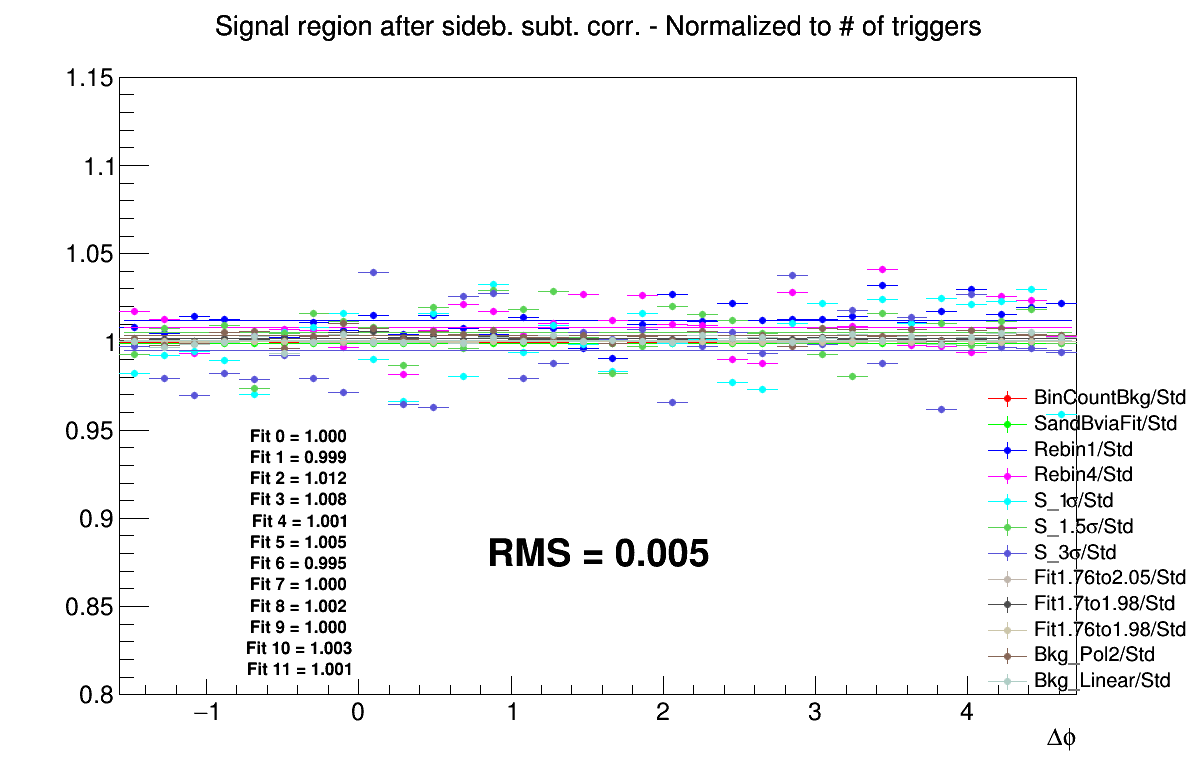
\includegraphics[width=0.31\linewidth]{Centrality_DPlus/Dplus/Systematic/0_20/Yield/Ratio_AzimCorrDistr_Dplus_Canvas_PtIntBins8to10_PoolInt_thrdot3to99dot.png}}
{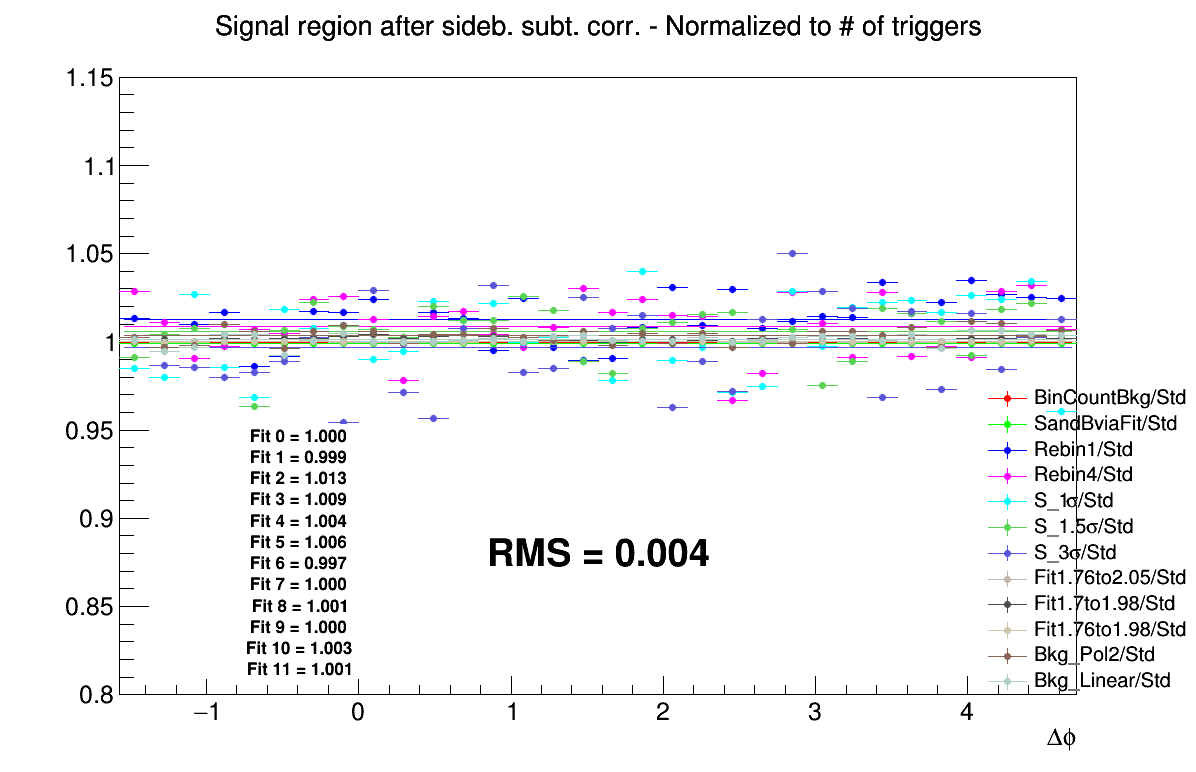
\includegraphics[width=0.31\linewidth]{Centrality_DPlus/Dplus/Systematic/0_20/Yield/Ratio_AzimCorrDistr_Dplus_Canvas_PtIntBins8to10_PoolInt_thrdot3to1dot.png}}
{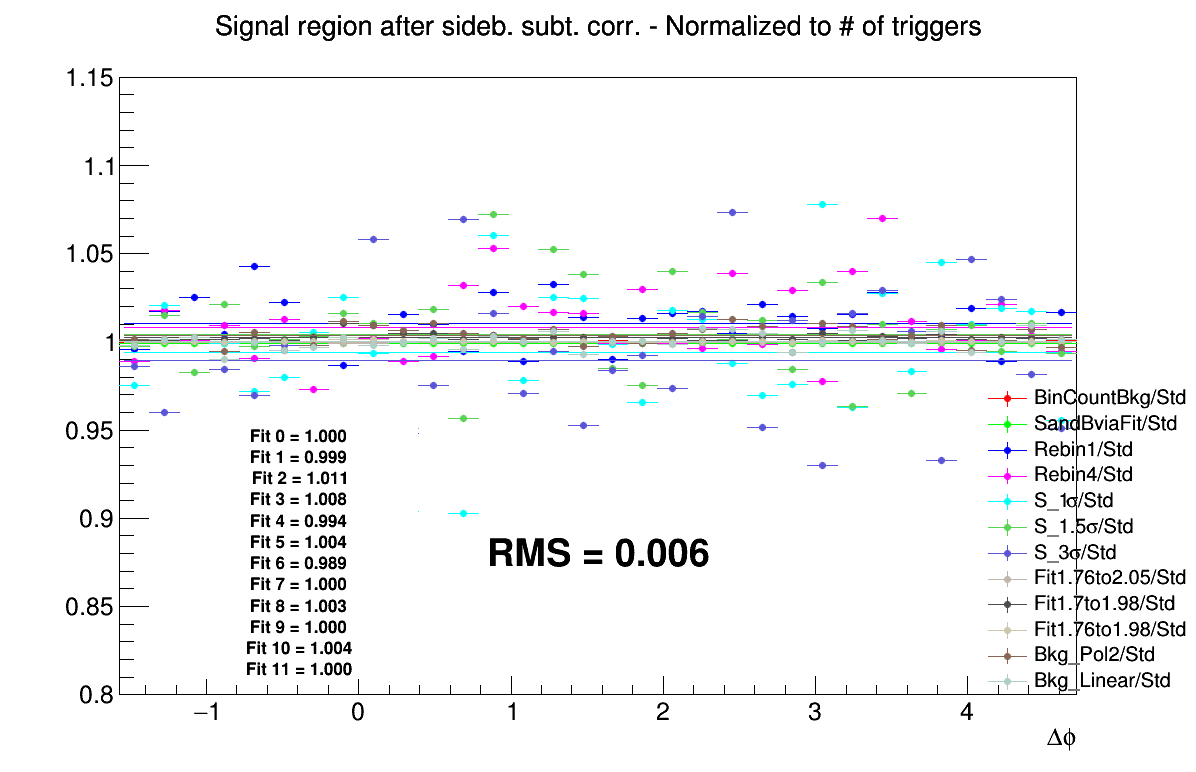
\includegraphics[width=0.31\linewidth]{Centrality_DPlus/Dplus/Systematic/0_20/Yield/Ratio_AzimCorrDistr_Dplus_Canvas_PtIntBins8to10_PoolInt_thr1dotto99dot.png}} \\
{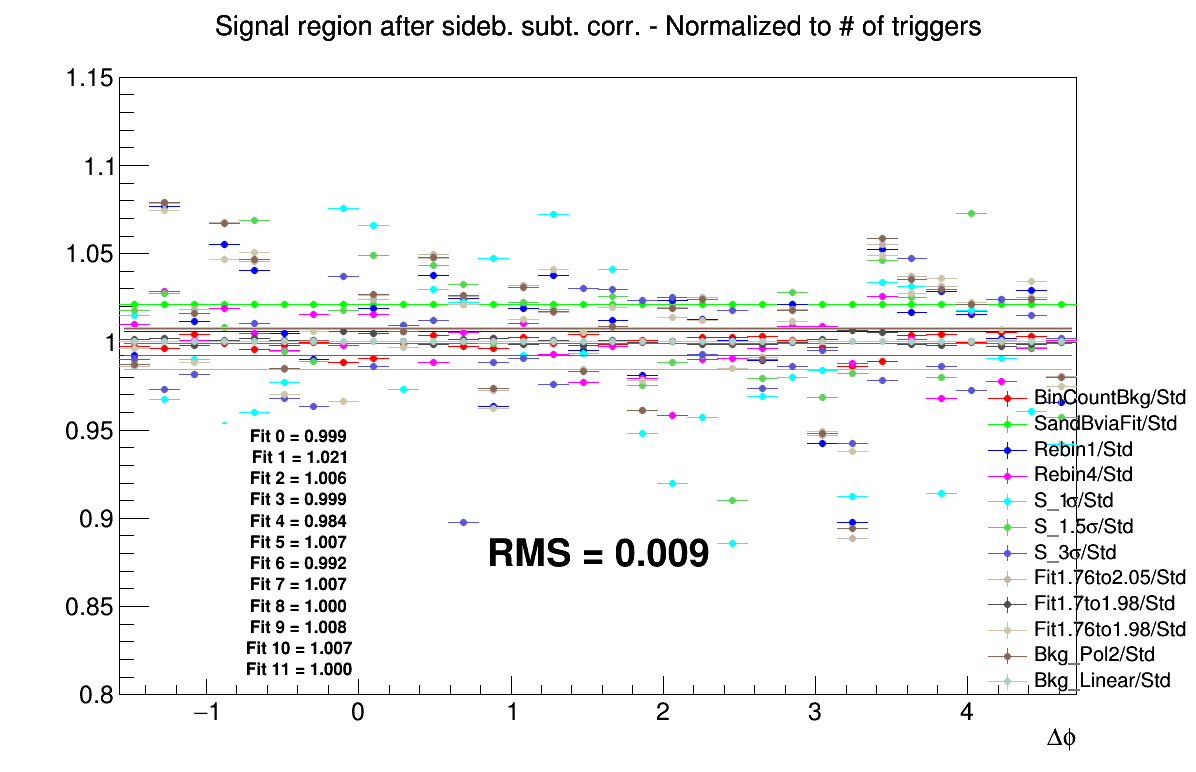
\includegraphics[width=0.31\linewidth]{Centrality_DPlus/Dplus/Systematic/0_20/Yield/Ratio_AzimCorrDistr_Dplus_Canvas_PtIntBins11to11_PoolInt_thrdot3to99dot.png}}
{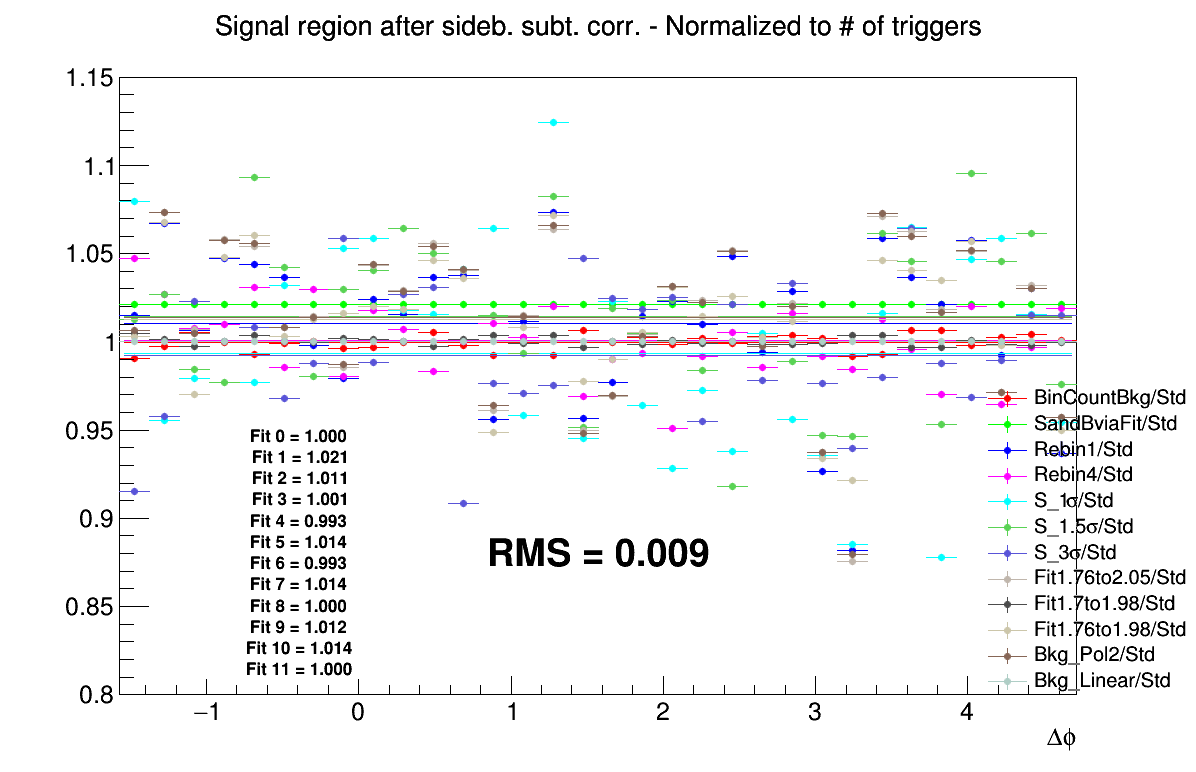
\includegraphics[width=0.31\linewidth]{Centrality_DPlus/Dplus/Systematic/0_20/Yield/Ratio_AzimCorrDistr_Dplus_Canvas_PtIntBins11to11_PoolInt_thrdot3to1dot.png}}
{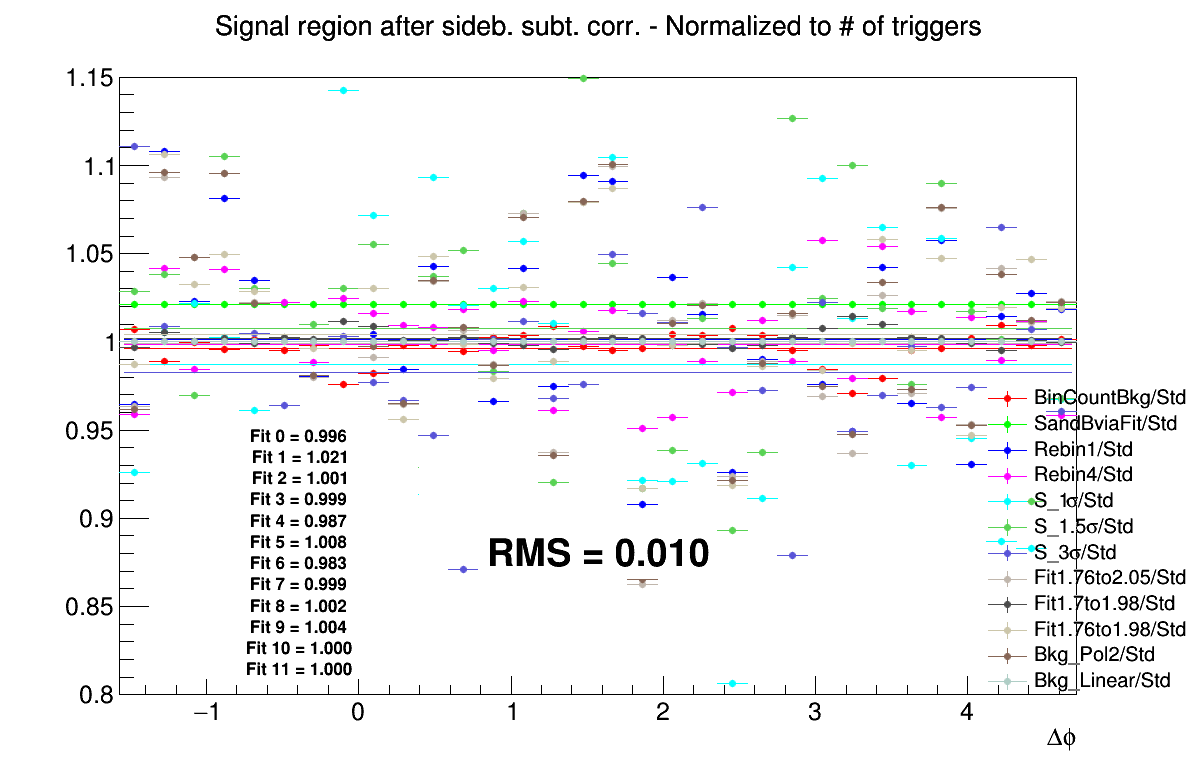
\includegraphics[width=0.31\linewidth]{Centrality_DPlus/Dplus/Systematic/0_20/Yield/Ratio_AzimCorrDistr_Dplus_Canvas_PtIntBins11to11_PoolInt_thr1dotto99dot.png}} \\
 \caption{Ratios of $\Dplus$-h correlation plots obtained with alternate S and B extraction approaches over those obtained with the standard procedure. For 0-20\% centrality. Rows: $\pt$($\Dplus$) 3-5, 5-8, 8-16, 16-24 GeV/$c$. In each row, the panels show the associated track
$\pt$ ranges $> 0.3$, 0.3-1, $> 1$ GeV/$c$, respectively.}
\label{fig:SysSandB020_Dplus}
\end{figure}

\begin{figure}
\centering
{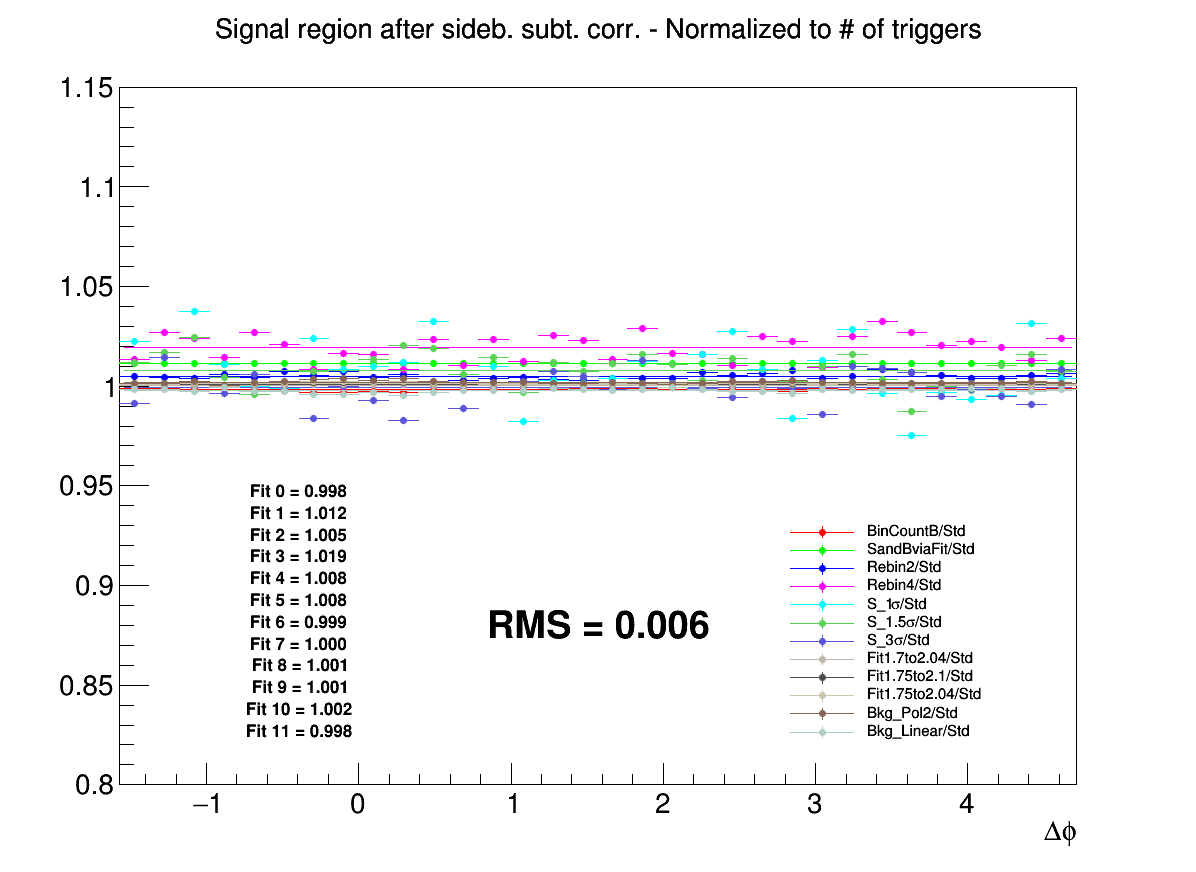
\includegraphics[width=0.31\linewidth]{figuresVsCent/Dzero/SystSandB/20_60/Ratio_AzimCorrDistr_Dzero_Canvas_PtIntBins4to5_PoolInt_thr03to99.png}}
{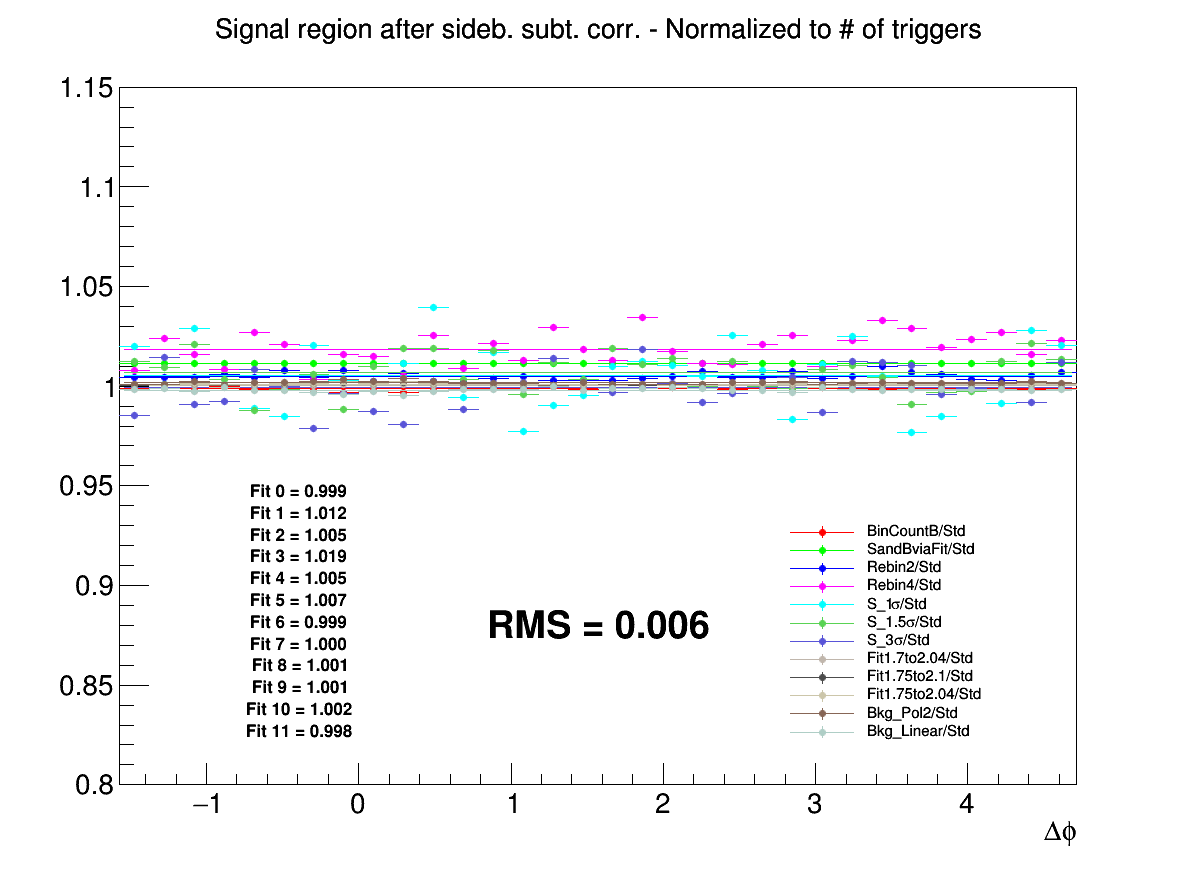
\includegraphics[width=0.31\linewidth]{figuresVsCent/Dzero/SystSandB/20_60/Ratio_AzimCorrDistr_Dzero_Canvas_PtIntBins4to5_PoolInt_thr03to1.png}}
{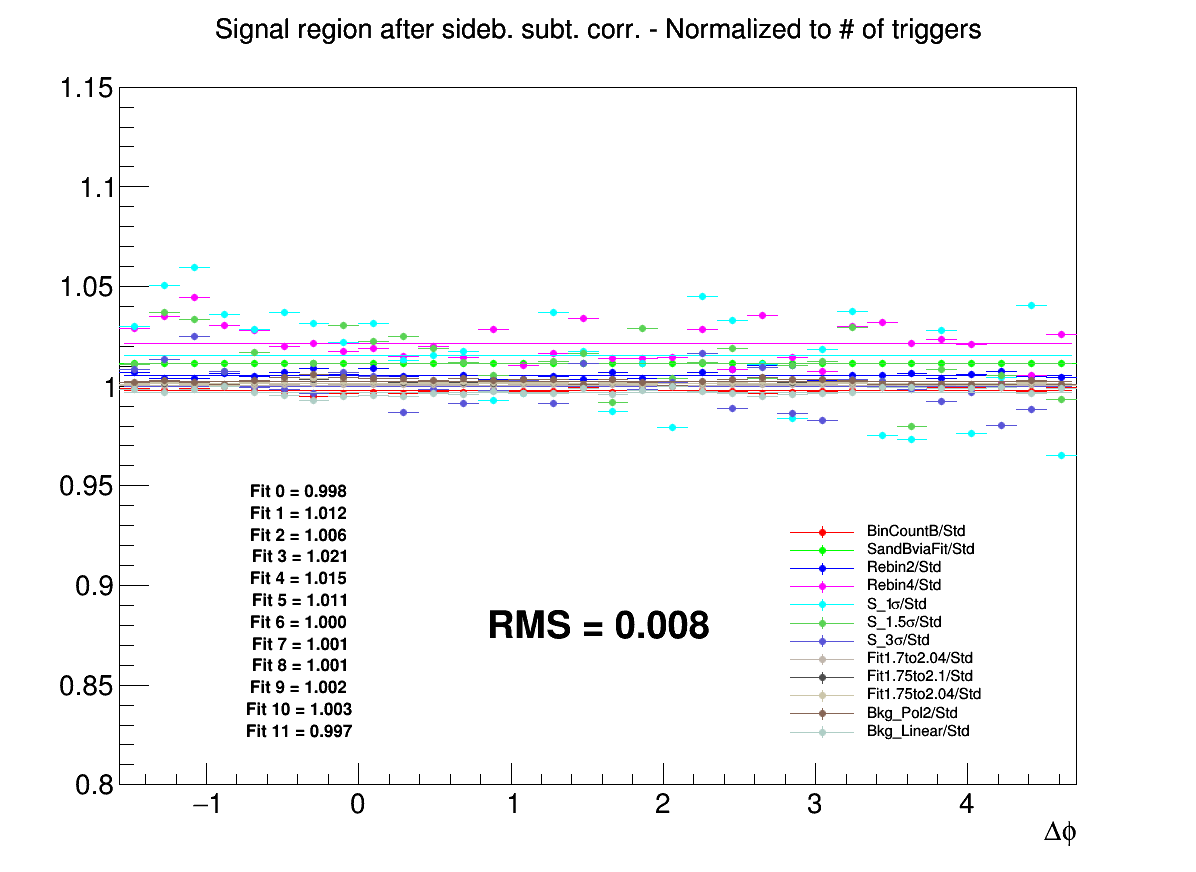
\includegraphics[width=0.31\linewidth]{figuresVsCent/Dzero/SystSandB/20_60/Ratio_AzimCorrDistr_Dzero_Canvas_PtIntBins4to5_PoolInt_thr1to99.png}} \\
{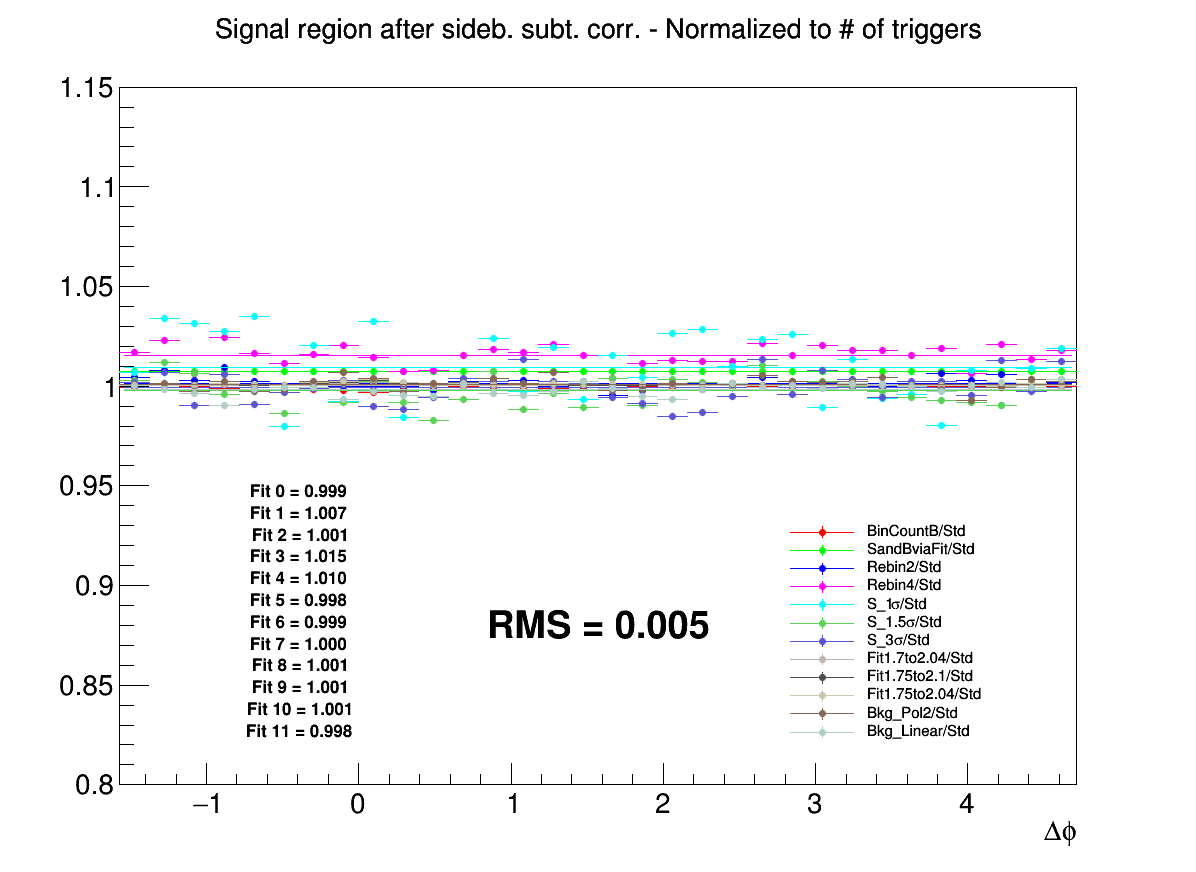
\includegraphics[width=0.31\linewidth]{figuresVsCent/Dzero/SystSandB/20_60/Ratio_AzimCorrDistr_Dzero_Canvas_PtIntBins6to8_PoolInt_thr03to99.png}}
{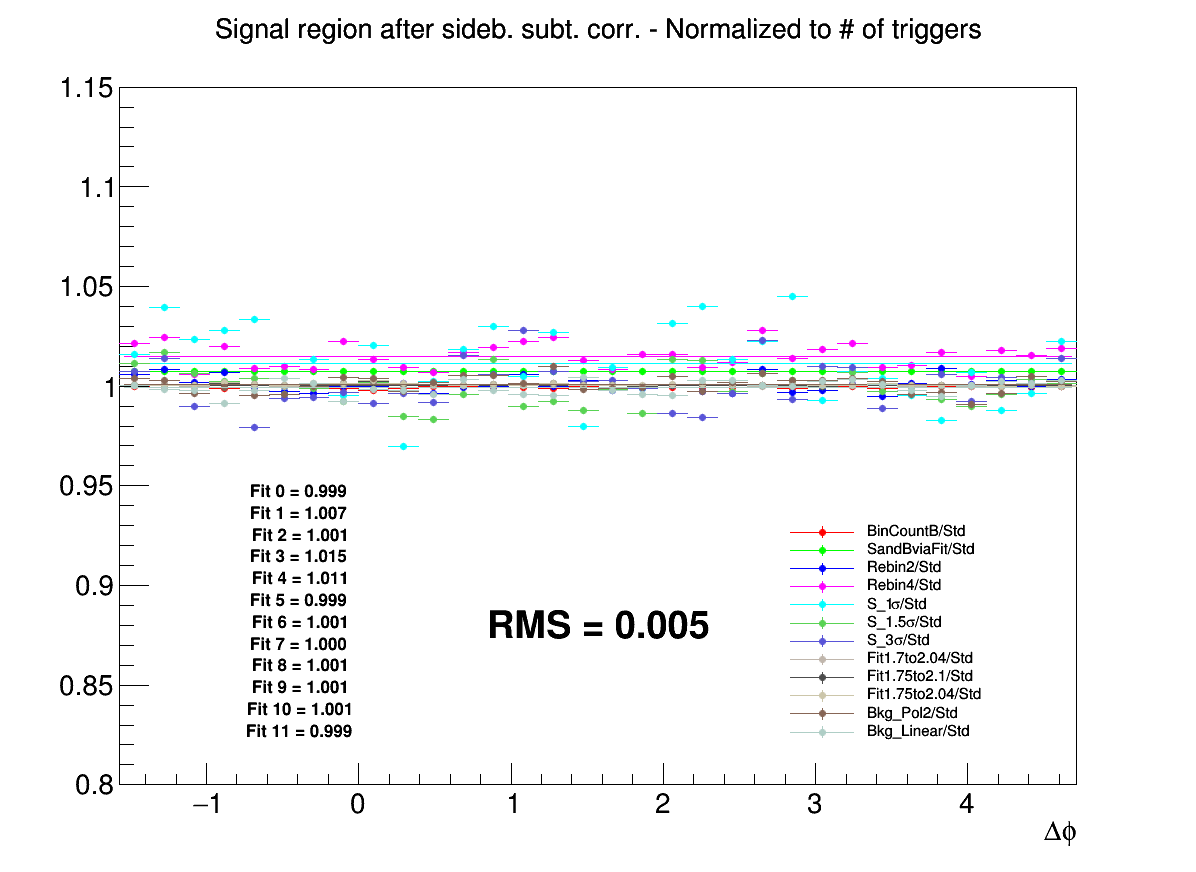
\includegraphics[width=0.31\linewidth]{figuresVsCent/Dzero/SystSandB/20_60/Ratio_AzimCorrDistr_Dzero_Canvas_PtIntBins6to8_PoolInt_thr03to1.png}}
{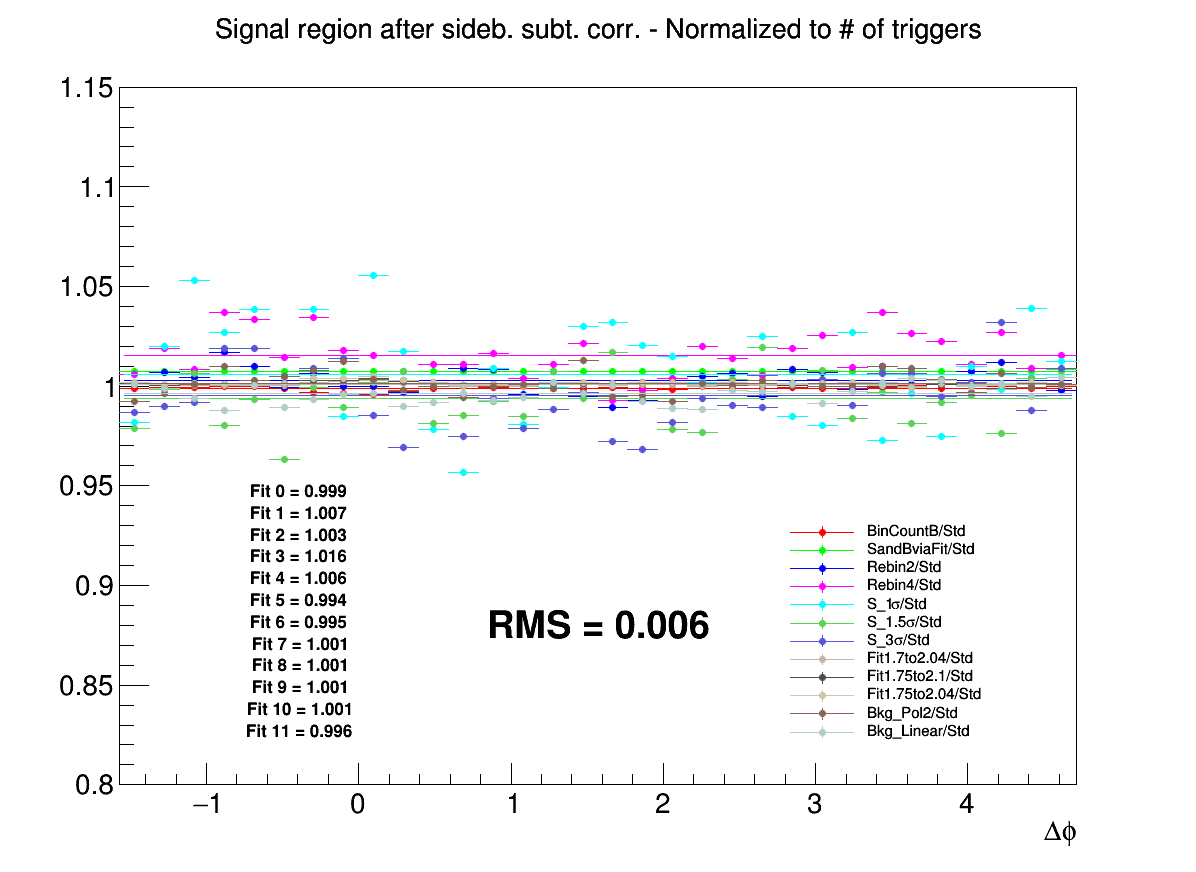
\includegraphics[width=0.31\linewidth]{figuresVsCent/Dzero/SystSandB/20_60/Ratio_AzimCorrDistr_Dzero_Canvas_PtIntBins6to8_PoolInt_thr1to99.png}} \\
{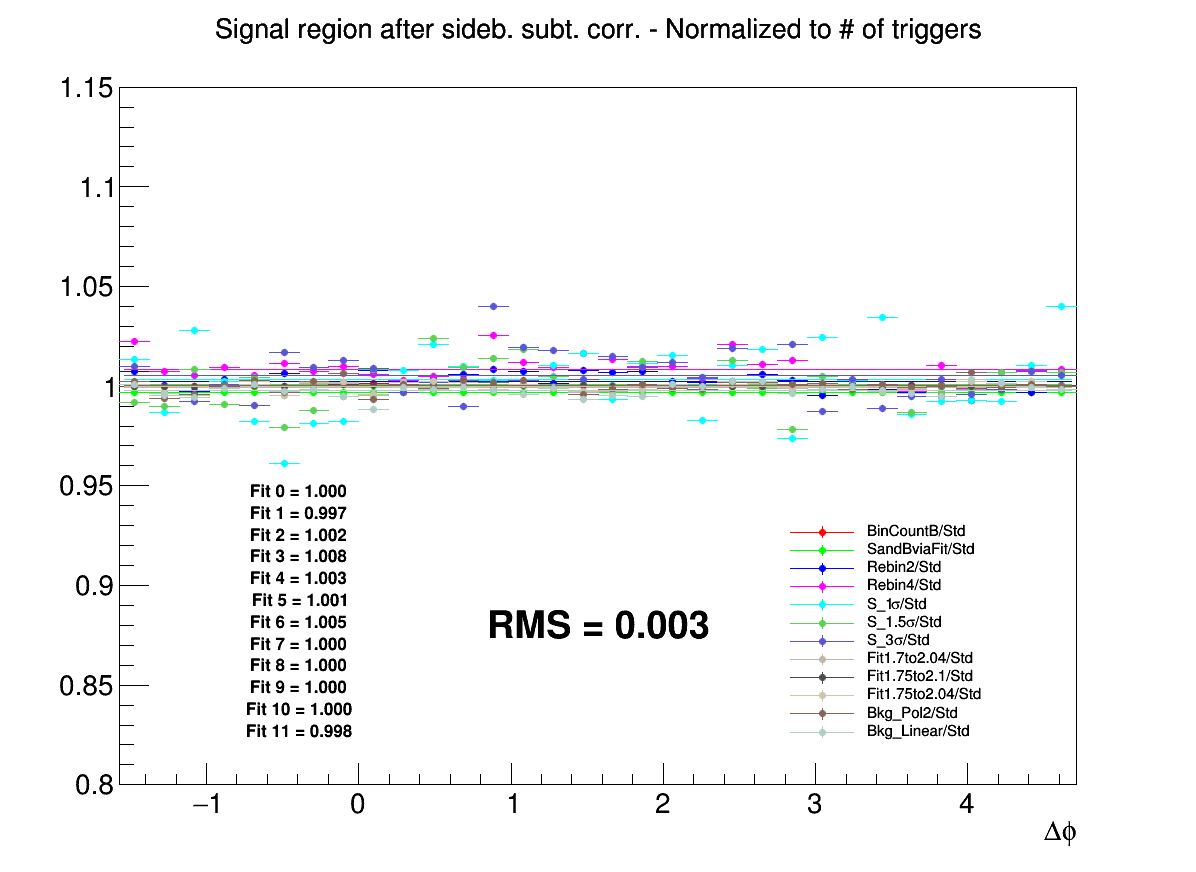
\includegraphics[width=0.31\linewidth]{figuresVsCent/Dzero/SystSandB/20_60/Ratio_AzimCorrDistr_Dzero_Canvas_PtIntBins9to11_PoolInt_thr03to99.png}}
{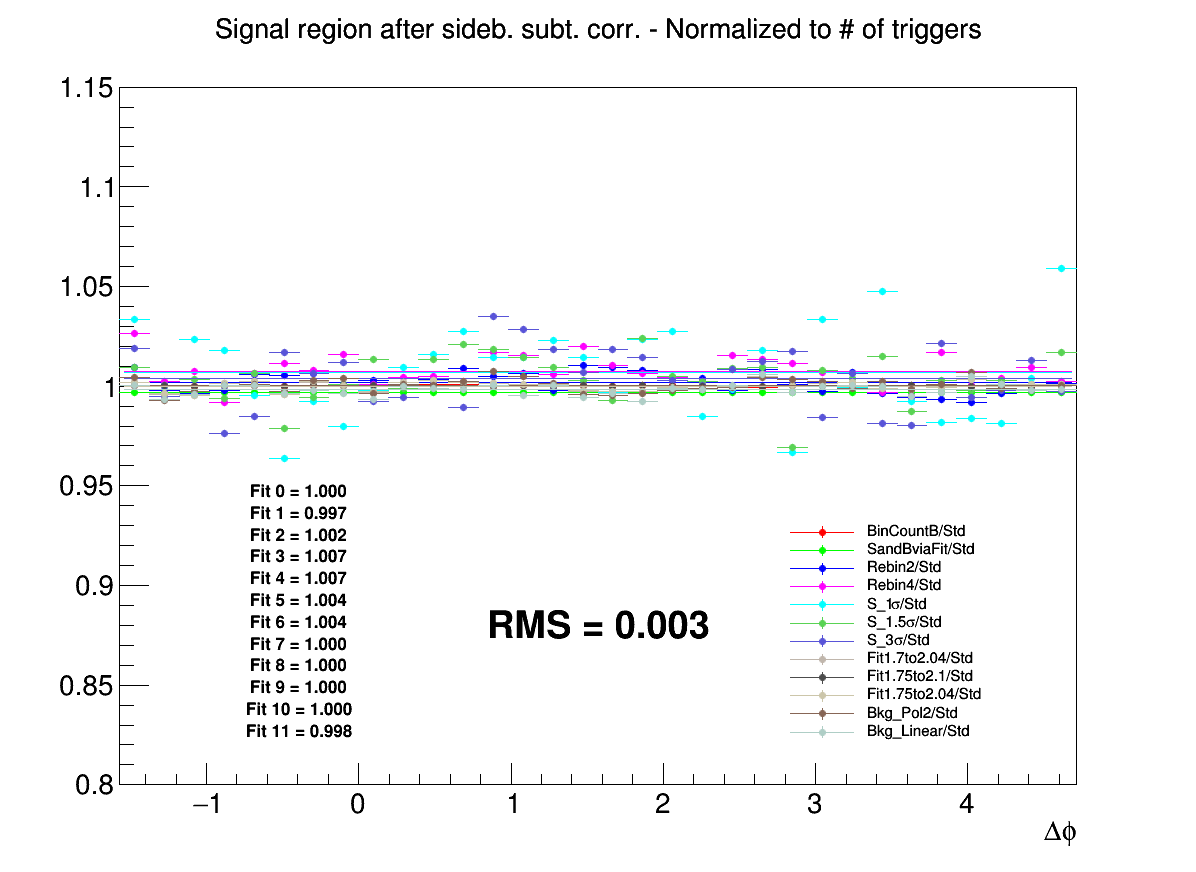
\includegraphics[width=0.31\linewidth]{figuresVsCent/Dzero/SystSandB/20_60/Ratio_AzimCorrDistr_Dzero_Canvas_PtIntBins9to11_PoolInt_thr03to1.png}}
{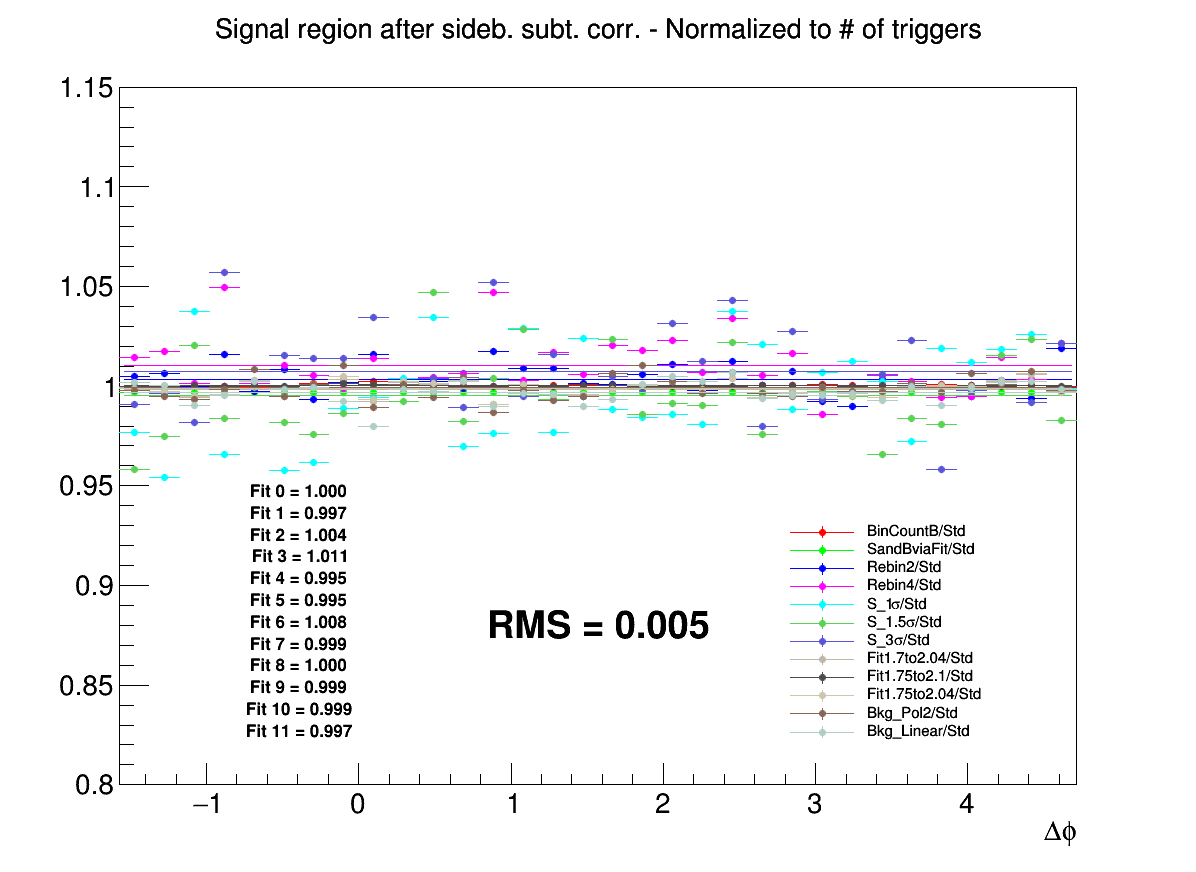
\includegraphics[width=0.31\linewidth]{figuresVsCent/Dzero/SystSandB/20_60/Ratio_AzimCorrDistr_Dzero_Canvas_PtIntBins9to11_PoolInt_thr1to99.png}} \\
{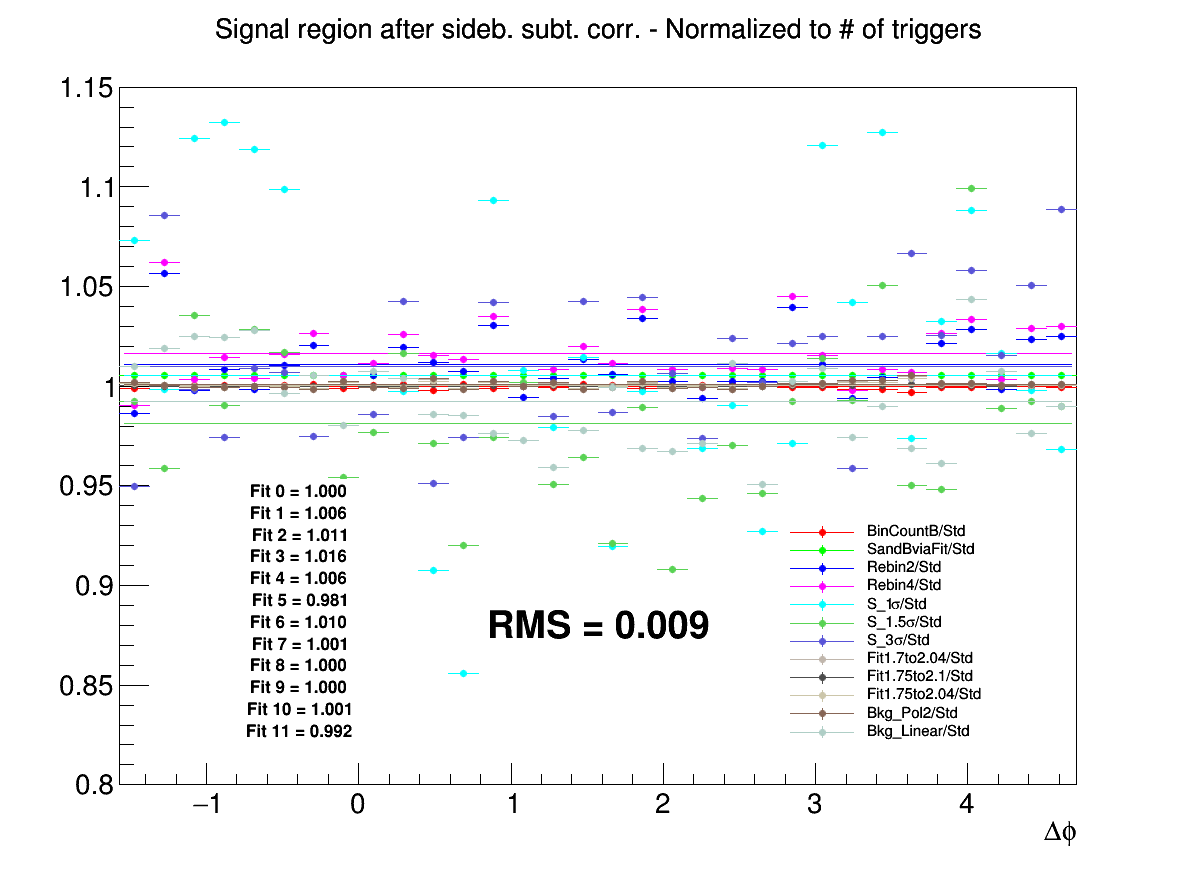
\includegraphics[width=0.31\linewidth]{figuresVsCent/Dzero/SystSandB/20_60/Ratio_AzimCorrDistr_Dzero_Canvas_PtIntBins12to12_PoolInt_thr03to99.png}}
{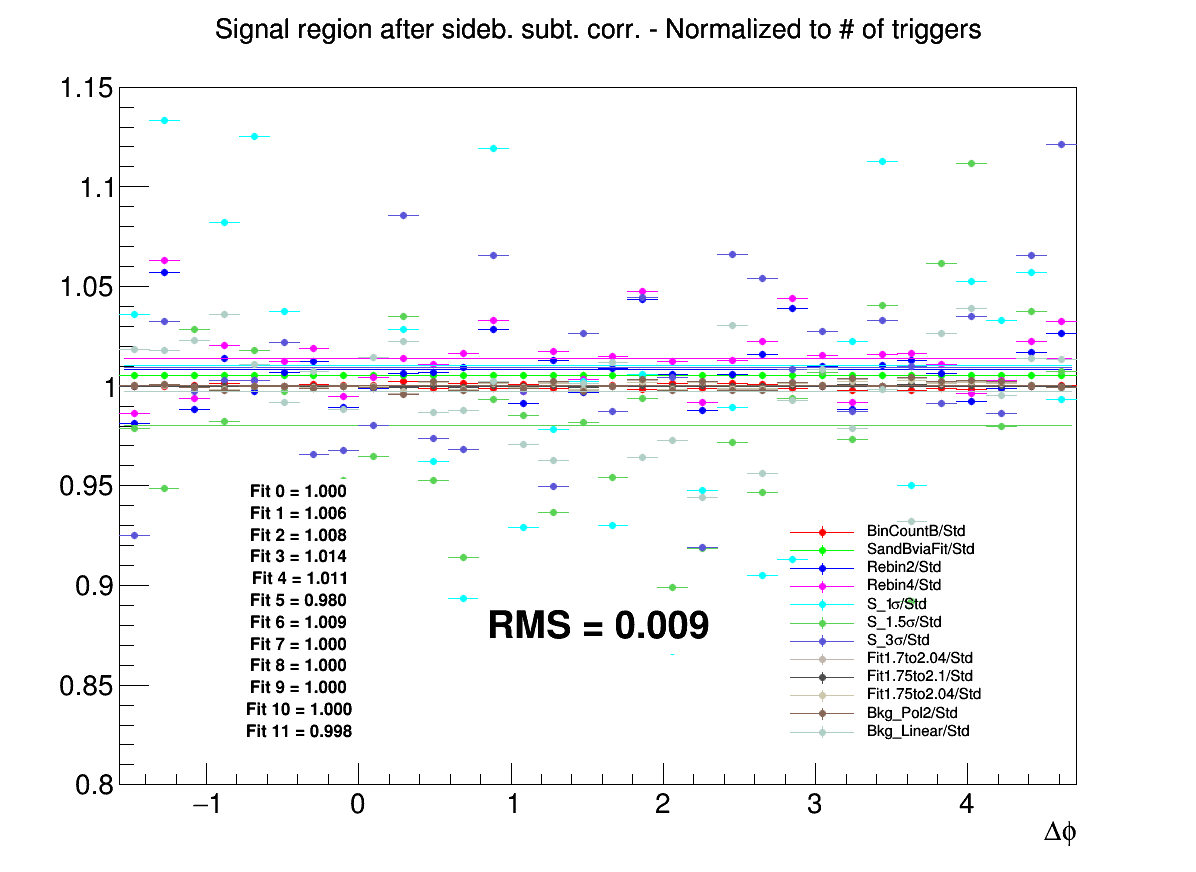
\includegraphics[width=0.31\linewidth]{figuresVsCent/Dzero/SystSandB/20_60/Ratio_AzimCorrDistr_Dzero_Canvas_PtIntBins12to12_PoolInt_thr03to1.png}}
{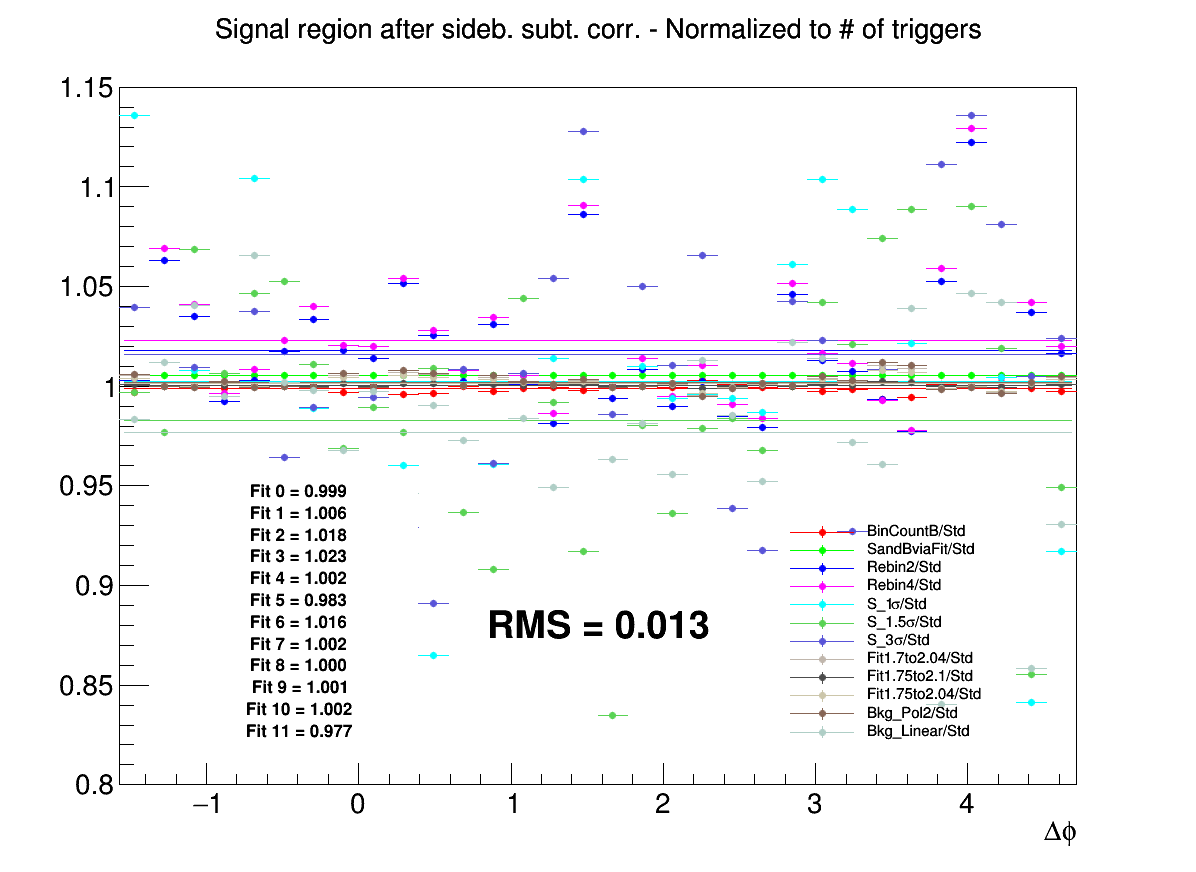
\includegraphics[width=0.31\linewidth]{figuresVsCent/Dzero/SystSandB/20_60/Ratio_AzimCorrDistr_Dzero_Canvas_PtIntBins12to12_PoolInt_thr1to99.png}} \\
 \caption{Ratios of $\Dzero$-h correlation plots obtained with alternate S and B extraction approaches over those obtained with the standard procedure. For 20-60\% centrality. Rows: $\pt$($\Dzero$) 3-5, 5-8, 8-16, 16-24 GeV/$c$. In each row, the panels show the associated track
$\pt$ ranges $> 0.3$, 0.3-1, $> 1$ GeV/$c$, respectively.}
\label{fig:SysSandB2060}
\end{figure}
% 20_60% Dplus Systematics
\begin{figure}
\centering
{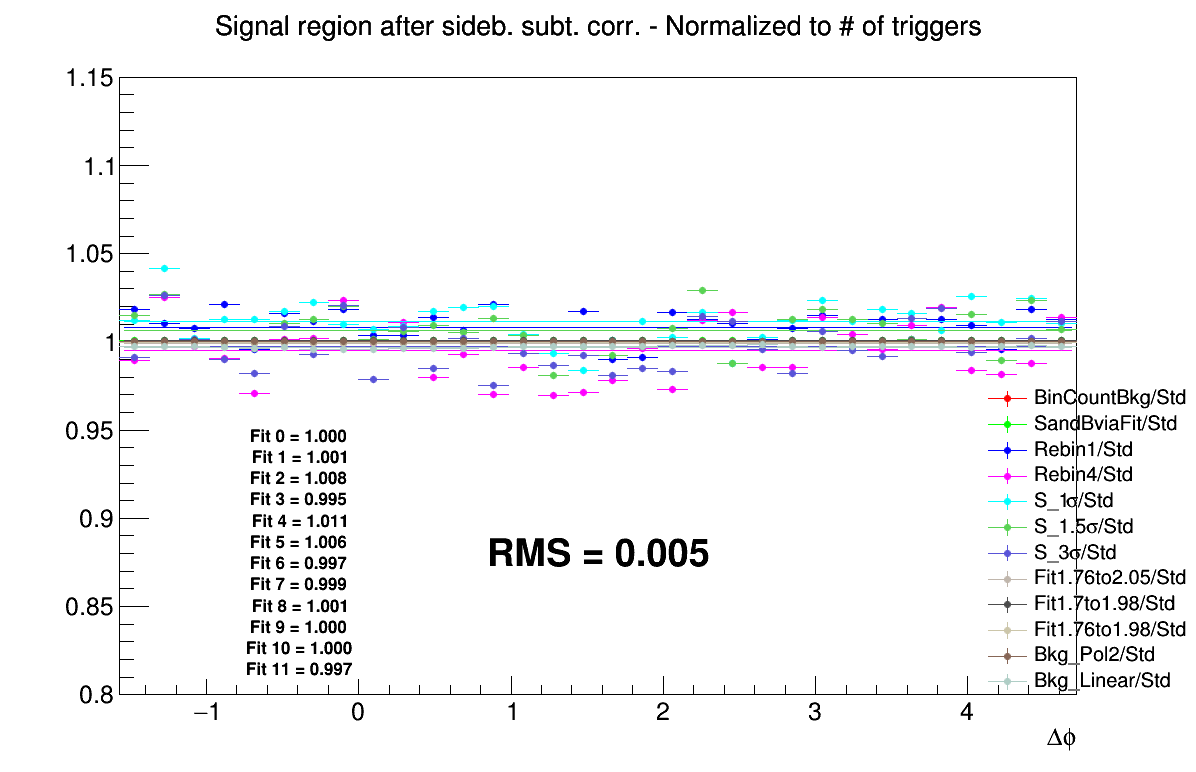
\includegraphics[width=0.31\linewidth]{Centrality_DPlus/Dplus/Systematic/20_60/Yield/Ratio_AzimCorrDistr_Dplus_Canvas_PtIntBins3to4_PoolInt_thrdot3to99dot.png}}
{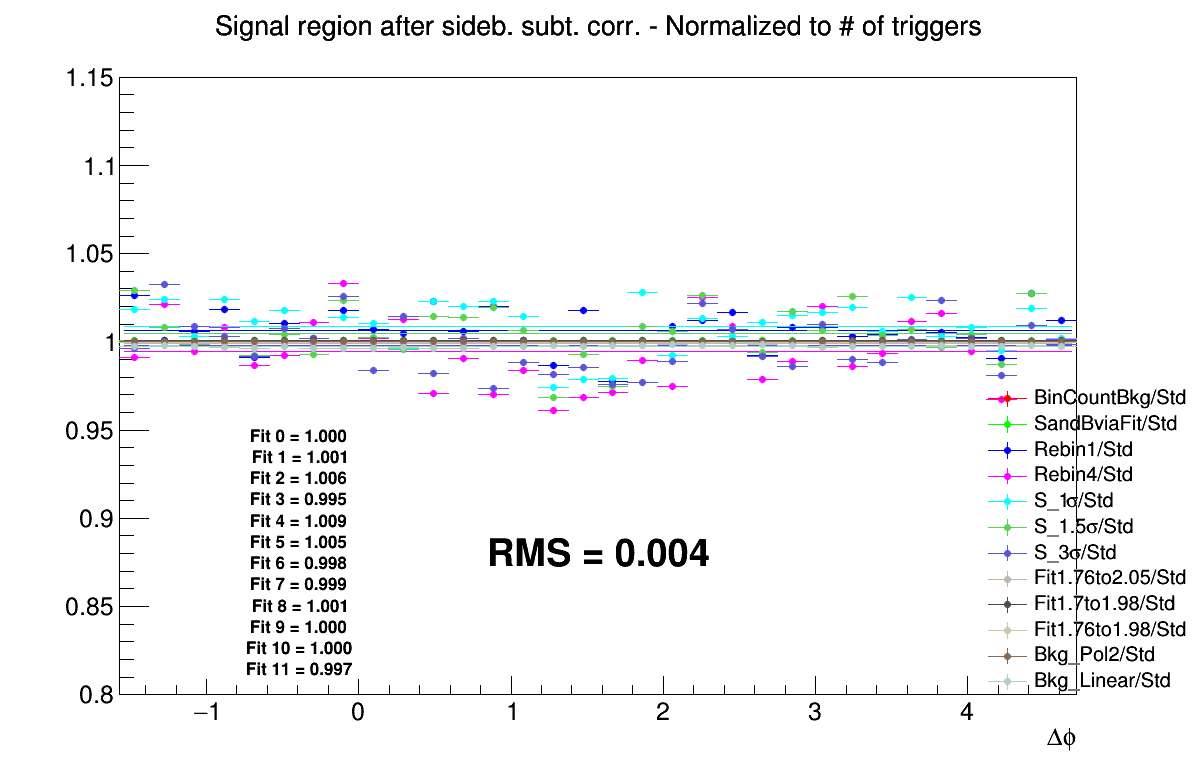
\includegraphics[width=0.31\linewidth]{Centrality_DPlus/Dplus/Systematic/20_60/Yield/Ratio_AzimCorrDistr_Dplus_Canvas_PtIntBins3to4_PoolInt_thrdot3to1dot.png}}
{\includegraphics[width=0.31\linewidth]{Centrality_DPlus/Dplus/Systematic/20_60/Yield/Ratio_AzimCorrDistr_Dplus_Canvas_PtIntBins3to4_PoolInt_thr1dotto99dot.png}} \\
{\includegraphics[width=0.31\linewidth]{Centrality_DPlus/Dplus/Systematic/20_60/Yield/Ratio_AzimCorrDistr_Dplus_Canvas_PtIntBins5to7_PoolInt_thrdot3to99dot.png}}
{\includegraphics[width=0.31\linewidth]{Centrality_DPlus/Dplus/Systematic/20_60/Yield/Ratio_AzimCorrDistr_Dplus_Canvas_PtIntBins5to7_PoolInt_thrdot3to1dot.png}}
{\includegraphics[width=0.31\linewidth]{Centrality_DPlus/Dplus/Systematic/20_60/Yield/Ratio_AzimCorrDistr_Dplus_Canvas_PtIntBins5to7_PoolInt_thr1dotto99dot.png}} \\
{\includegraphics[width=0.31\linewidth]{Centrality_DPlus/Dplus/Systematic/20_60/Yield/Ratio_AzimCorrDistr_Dplus_Canvas_PtIntBins8to10_PoolInt_thrdot3to99dot.png}}
{\includegraphics[width=0.31\linewidth]{Centrality_DPlus/Dplus/Systematic/20_60/Yield/Ratio_AzimCorrDistr_Dplus_Canvas_PtIntBins8to10_PoolInt_thrdot3to1dot.png}}
{\includegraphics[width=0.31\linewidth]{Centrality_DPlus/Dplus/Systematic/20_60/Yield/Ratio_AzimCorrDistr_Dplus_Canvas_PtIntBins8to10_PoolInt_thr1dotto99dot.png}} \\
{\includegraphics[width=0.31\linewidth]{Centrality_DPlus/Dplus/Systematic/20_60/Yield/Ratio_AzimCorrDistr_Dplus_Canvas_PtIntBins11to11_PoolInt_thrdot3to99dot.png}}
{\includegraphics[width=0.31\linewidth]{Centrality_DPlus/Dplus/Systematic/20_60/Yield/Ratio_AzimCorrDistr_Dplus_Canvas_PtIntBins11to11_PoolInt_thrdot3to1dot.png}}
{\includegraphics[width=0.31\linewidth]{Centrality_DPlus/Dplus/Systematic/20_60/Yield/Ratio_AzimCorrDistr_Dplus_Canvas_PtIntBins11to11_PoolInt_thr1dotto99dot.png}} \\
 \caption{Ratios of $\Dplus$-h correlation plots obtained with alternate S and B extraction approaches over those obtained with the standard procedure. For 20-60\% centrality. Rows: $\pt$($\Dplus$) 3-5, 5-8, 8-16, 16-24 GeV/$c$. In each row, the panels show the associated track
$\pt$ ranges $> 0.3$, 0.3-1, $> 1$ GeV/$c$, respectively.}
\label{fig:SysSandB2060_Dplus}
\end{figure}

\begin{figure}
\centering
{\includegraphics[width=0.31\linewidth]{figuresVsCent/Dstar/SystSandB/2060_SandB_Syst/Ratio_AzimCorrDistr_Dstar_Canvas_PtIntBins2to3_PoolInt_thr03to99_YIELD_2060.png}}
{\includegraphics[width=0.31\linewidth]{figuresVsCent/Dstar/SystSandB/2060_SandB_Syst/Ratio_AzimCorrDistr_Dstar_Canvas_PtIntBins2to3_PoolInt_thr03to1_YIELD_2060.png}}
{\includegraphics[width=0.31\linewidth]{figuresVsCent/Dstar/SystSandB/2060_SandB_Syst/Ratio_AzimCorrDistr_Dstar_Canvas_PtIntBins2to3_PoolInt_thr1to99_YIELD_2060.png}} \\

{\includegraphics[width=0.31\linewidth]{figuresVsCent/Dstar/SystSandB/2060_SandB_Syst/Ratio_AzimCorrDistr_Dstar_Canvas_PtIntBins4to6_PoolInt_thr03to99_YIELD_2060.png}}
{\includegraphics[width=0.31\linewidth]{figuresVsCent/Dstar/SystSandB/2060_SandB_Syst/Ratio_AzimCorrDistr_Dstar_Canvas_PtIntBins4to6_PoolInt_thr03to1_YIELD_2060.png}}
{\includegraphics[width=0.31\linewidth]{figuresVsCent/Dstar/SystSandB/2060_SandB_Syst/Ratio_AzimCorrDistr_Dstar_Canvas_PtIntBins4to6_PoolInt_thr1to99_YIELD_2060.png}} \\

{\includegraphics[width=0.31\linewidth]{figuresVsCent/Dstar/SystSandB/2060_SandB_Syst/Ratio_AzimCorrDistr_Dstar_Canvas_PtIntBins7to9_PoolInt_thr03to99_YIELD_2060.png}}
{\includegraphics[width=0.31\linewidth]{figuresVsCent/Dstar/SystSandB/2060_SandB_Syst/Ratio_AzimCorrDistr_Dstar_Canvas_PtIntBins7to9_PoolInt_thr03to1_YIELD_2060.png}}
{\includegraphics[width=0.31\linewidth]{figuresVsCent/Dstar/SystSandB/2060_SandB_Syst/Ratio_AzimCorrDistr_Dstar_Canvas_PtIntBins7to9_PoolInt_thr1to99_YIELD_2060.png}} \\

{\includegraphics[width=0.31\linewidth]{figuresVsCent/Dstar/SystSandB/2060_SandB_Syst/Ratio_AzimCorrDistr_Dstar_Canvas_PtIntBins10to10_PoolInt_thr03to99_YIELD_2060.png}}
{\includegraphics[width=0.31\linewidth]{figuresVsCent/Dstar/SystSandB/2060_SandB_Syst/Ratio_AzimCorrDistr_Dstar_Canvas_PtIntBins10to10_PoolInt_thr03to1_YIELD_2060.png}}
{\includegraphics[width=0.31\linewidth]{figuresVsCent/Dstar/SystSandB/2060_SandB_Syst/Ratio_AzimCorrDistr_Dstar_Canvas_PtIntBins10to10_PoolInt_thr1to99_YIELD_2060.png}} \\
 \caption{Ratios of $\Dstar$-h correlation plots obtained with alternate S and B extraction approaches over those obtained with the standard procedure. For 20-60\% centrality. Rows: $\pt$($\Dstar$) 3-5, 5-8, 8-16, 16-24 GeV/$c$. In each row, the panels show the associated track
$\pt$ ranges $> 0.3$, 0.3-1, $> 1$ GeV/$c$, respectively.}
\label{fig:SysSandB2060Dstar}
\end{figure}


\begin{figure}
\centering
{\includegraphics[width=0.31\linewidth]{figuresVsCent/Dzero/SystSandB/60_100/Ratio_AzimCorrDistr_Dzero_Canvas_PtIntBins4to5_PoolInt_thr03to99.png}}
{\includegraphics[width=0.31\linewidth]{figuresVsCent/Dzero/SystSandB/60_100/Ratio_AzimCorrDistr_Dzero_Canvas_PtIntBins4to5_PoolInt_thr03to1.png}}
{\includegraphics[width=0.31\linewidth]{figuresVsCent/Dzero/SystSandB/60_100/Ratio_AzimCorrDistr_Dzero_Canvas_PtIntBins4to5_PoolInt_thr1to99.png}} \\
{\includegraphics[width=0.31\linewidth]{figuresVsCent/Dzero/SystSandB/60_100/Ratio_AzimCorrDistr_Dzero_Canvas_PtIntBins6to8_PoolInt_thr03to99.png}}
{\includegraphics[width=0.31\linewidth]{figuresVsCent/Dzero/SystSandB/60_100/Ratio_AzimCorrDistr_Dzero_Canvas_PtIntBins6to8_PoolInt_thr03to1.png}}
{\includegraphics[width=0.31\linewidth]{figuresVsCent/Dzero/SystSandB/60_100/Ratio_AzimCorrDistr_Dzero_Canvas_PtIntBins6to8_PoolInt_thr1to99.png}} \\
{\includegraphics[width=0.31\linewidth]{figuresVsCent/Dzero/SystSandB/60_100/Ratio_AzimCorrDistr_Dzero_Canvas_PtIntBins9to11_PoolInt_thr03to99.png}}
{\includegraphics[width=0.31\linewidth]{figuresVsCent/Dzero/SystSandB/60_100/Ratio_AzimCorrDistr_Dzero_Canvas_PtIntBins9to11_PoolInt_thr03to1.png}}
{\includegraphics[width=0.31\linewidth]{figuresVsCent/Dzero/SystSandB/60_100/Ratio_AzimCorrDistr_Dzero_Canvas_PtIntBins9to11_PoolInt_thr1to99.png}} \\
{\includegraphics[width=0.31\linewidth]{figuresVsCent/Dzero/SystSandB/60_100/Ratio_AzimCorrDistr_Dzero_Canvas_PtIntBins12to12_PoolInt_thr03to99.png}}
{\includegraphics[width=0.31\linewidth]{figuresVsCent/Dzero/SystSandB/60_100/Ratio_AzimCorrDistr_Dzero_Canvas_PtIntBins12to12_PoolInt_thr03to1.png}}
{\includegraphics[width=0.31\linewidth]{figuresVsCent/Dzero/SystSandB/60_100/Ratio_AzimCorrDistr_Dzero_Canvas_PtIntBins12to12_PoolInt_thr1to99.png}} \\
 \caption{Ratios of $\Dzero$-h correlation plots obtained with alternate S and B extraction approaches over those obtained with the standard procedure. For 60-100\% centrality. Rows: $\pt$($\Dzero$) 3-5, 5-8, 8-16, 16-24 GeV/$c$. In each row, the panels show the associated track
$\pt$ ranges $> 0.3$, 0.3-1, $> 1$ GeV/$c$, respectively.}
\label{fig:SysSandB60100}
\end{figure}
% 60_100% Dplus Systematics
\begin{figure}
\centering
{\includegraphics[width=0.31\linewidth]{Centrality_DPlus/Dplus/Systematic/60_100/Yield/Ratio_AzimCorrDistr_Dplus_Canvas_PtIntBins3to4_PoolInt_thrdot3to99dot.png}}
{\includegraphics[width=0.31\linewidth]{Centrality_DPlus/Dplus/Systematic/60_100/Yield/Ratio_AzimCorrDistr_Dplus_Canvas_PtIntBins3to4_PoolInt_thrdot3to1dot.png}}
{\includegraphics[width=0.31\linewidth]{Centrality_DPlus/Dplus/Systematic/60_100/Yield/Ratio_AzimCorrDistr_Dplus_Canvas_PtIntBins3to4_PoolInt_thr1dotto99dot.png}} \\
{\includegraphics[width=0.31\linewidth]{Centrality_DPlus/Dplus/Systematic/60_100/Yield/Ratio_AzimCorrDistr_Dplus_Canvas_PtIntBins5to7_PoolInt_thrdot3to99dot.png}}
{\includegraphics[width=0.31\linewidth]{Centrality_DPlus/Dplus/Systematic/60_100/Yield/Ratio_AzimCorrDistr_Dplus_Canvas_PtIntBins5to7_PoolInt_thrdot3to1dot.png}}
{\includegraphics[width=0.31\linewidth]{Centrality_DPlus/Dplus/Systematic/60_100/Yield/Ratio_AzimCorrDistr_Dplus_Canvas_PtIntBins5to7_PoolInt_thr1dotto99dot.png}} \\
{\includegraphics[width=0.31\linewidth]{Centrality_DPlus/Dplus/Systematic/60_100/Yield/Ratio_AzimCorrDistr_Dplus_Canvas_PtIntBins8to10_PoolInt_thrdot3to99dot.png}}
{\includegraphics[width=0.31\linewidth]{Centrality_DPlus/Dplus/Systematic/60_100/Yield/Ratio_AzimCorrDistr_Dplus_Canvas_PtIntBins8to10_PoolInt_thrdot3to1dot.png}}
{\includegraphics[width=0.31\linewidth]{Centrality_DPlus/Dplus/Systematic/60_100/Yield/Ratio_AzimCorrDistr_Dplus_Canvas_PtIntBins8to10_PoolInt_thr1dotto99dot.png}} \\
{\includegraphics[width=0.31\linewidth]{Centrality_DPlus/Dplus/Systematic/60_100/Yield/Ratio_AzimCorrDistr_Dplus_Canvas_PtIntBins11to11_PoolInt_thrdot3to99dot.png}}
{\includegraphics[width=0.31\linewidth]{Centrality_DPlus/Dplus/Systematic/60_100/Yield/Ratio_AzimCorrDistr_Dplus_Canvas_PtIntBins11to11_PoolInt_thrdot3to1dot.png}}
{\includegraphics[width=0.31\linewidth]{Centrality_DPlus/Dplus/Systematic/60_100/Yield/Ratio_AzimCorrDistr_Dplus_Canvas_PtIntBins11to11_PoolInt_thr1dotto99dot.png}} \\
 \caption{Ratios of $\Dplus$-h correlation plots obtained with alternate S and B extraction approaches over those obtained with the standard procedure. For 60-100\% centrality. Rows: $\pt$($\Dplus$) 3-5, 5-8, 8-16, 16-24 GeV/$c$. In each row, the panels show the associated track
$\pt$ ranges $> 0.3$, 0.3-1, $> 1$ GeV/$c$, respectively.}
\label{fig:SysSandB60100_Dplus}
\end{figure}


\begin{figure}
\centering
{\includegraphics[width=0.31\linewidth]{figuresVsCent/Dstar/SystSandB/60100_SandB_Syst/Ratio_AzimCorrDistr_Dstar_Canvas_PtIntBins2to3_PoolInt_thr03to99_YIELD_60100.png}}
{\includegraphics[width=0.31\linewidth]{figuresVsCent/Dstar/SystSandB/60100_SandB_Syst/Ratio_AzimCorrDistr_Dstar_Canvas_PtIntBins2to3_PoolInt_thr03to1_YIELD_60100.png}}
{\includegraphics[width=0.31\linewidth]{figuresVsCent/Dstar/SystSandB/60100_SandB_Syst/Ratio_AzimCorrDistr_Dstar_Canvas_PtIntBins2to3_PoolInt_thr1to99_YIELD_60100.png}} \\

{\includegraphics[width=0.31\linewidth]{figuresVsCent/Dstar/SystSandB/60100_SandB_Syst/Ratio_AzimCorrDistr_Dstar_Canvas_PtIntBins4to6_PoolInt_thr03to99_YIELD_60100.png}}
{\includegraphics[width=0.31\linewidth]{figuresVsCent/Dstar/SystSandB/60100_SandB_Syst/Ratio_AzimCorrDistr_Dstar_Canvas_PtIntBins4to6_PoolInt_thr03to1_YIELD_60100.png}}
{\includegraphics[width=0.31\linewidth]{figuresVsCent/Dstar/SystSandB/60100_SandB_Syst/Ratio_AzimCorrDistr_Dstar_Canvas_PtIntBins4to6_PoolInt_thr1to99_YIELD_60100.png}} \\

{\includegraphics[width=0.31\linewidth]{figuresVsCent/Dstar/SystSandB/60100_SandB_Syst/Ratio_AzimCorrDistr_Dstar_Canvas_PtIntBins7to9_PoolInt_thr03to99_YIELD_60100.png}}
{\includegraphics[width=0.31\linewidth]{figuresVsCent/Dstar/SystSandB/60100_SandB_Syst/Ratio_AzimCorrDistr_Dstar_Canvas_PtIntBins7to9_PoolInt_thr03to1_YIELD_60100.png}}
{\includegraphics[width=0.31\linewidth]{figuresVsCent/Dstar/SystSandB/60100_SandB_Syst/Ratio_AzimCorrDistr_Dstar_Canvas_PtIntBins7to9_PoolInt_thr1to99_YIELD_60100.png}} \\

{\includegraphics[width=0.31\linewidth]{figuresVsCent/Dstar/SystSandB/60100_SandB_Syst/Ratio_AzimCorrDistr_Dstar_Canvas_PtIntBins10to10_PoolInt_thr03to99_YIELD_60100.png}}
{\includegraphics[width=0.31\linewidth]{figuresVsCent/Dstar/SystSandB/60100_SandB_Syst/Ratio_AzimCorrDistr_Dstar_Canvas_PtIntBins10to10_PoolInt_thr03to1_YIELD_60100.png}}
{\includegraphics[width=0.31\linewidth]{figuresVsCent/Dstar/SystSandB/60100_SandB_Syst/Ratio_AzimCorrDistr_Dstar_Canvas_PtIntBins10to10_PoolInt_thr1to99_YIELD_60100.png}} \\
 \caption{Ratios of $\Dstar$-h correlation plots obtained with alternate S and B extraction approaches over those obtained with the standard procedure. For 60-100\% centrality. Rows: $\pt$($\Dstar$) 3-5, 5-8, 8-16, 16-24 GeV/$c$. In each row, the panels show the associated track
$\pt$ ranges $> 0.3$, 0.3-1, $> 1$ GeV/$c$, respectively.}
\label{fig:SysSandB60100Dstar}
\end{figure}
\clearpage

\subsubsection{Background correlation shape}
A systematic effect can arise from the an incorrect description of the background correlations, for background triggers under the signal peak, when correlations considered using sideband candidates are considered to mimic this contribution. An uncertainty is addressed by varying the range of the D-meson sidebands in the invariant mass spectra (differently for each D-meson specie), similarly to what shown in subsection 4.2.

The ratio of correlation distributions with alternate/standard sideband definition is shown in Figs. \ref{fig:SysBkg020}, \ref{fig:SysBkg2060}, \ref{fig:SysBkg60100} for the $\Dzero$ meson. The uncertainty assigned to this source is 1\% for $\pt$(D) $< 16$ GeV/$c$, and 2\% for $16 < \pt$(D) $< 24$ GeV/$c$ for 0-20\% and 20-60\%. For 60-100\%, the uncertainty is 2\% for all the kinematic ranges.
In Figs. \ref{fig:SysBkg020_Dstar}, \ref{fig:SysBkg2060_Dstar}, \ref{fig:SysBkg60100_Dstar} the ratio of correlation distributions with alternate/standard sideband definition is shown for the $\Dstar$ meson. The values of the systematic uncertainties assigned for this source are summarized in \ref{fig:TableSystDstar}.

In Figs. \ref{fig:SysBkg020_Dplus}, \ref{fig:SysBkg2060_Dplus}, \ref{fig:SysBkg60100_Dplus} the ratio of correlation distributions with alternate/standard sideband definition is shown for the $\Dplus$ meson. The values of the systematic uncertainties assigned for this source are summarized in \ref{fig:TableSystDplus}.

\begin{figure}
\centering
{\includegraphics[width=0.31\linewidth]{figuresVsCent/Dzero/SystSideb/020/Ratio_AzimCorrDistr_Dzero_Canvas_PtIntBins4to5_PoolInt_thr03to99.png}}
{\includegraphics[width=0.31\linewidth]{figuresVsCent/Dzero/SystSideb/020/Ratio_AzimCorrDistr_Dzero_Canvas_PtIntBins4to5_PoolInt_thr03to1.png}}
{\includegraphics[width=0.31\linewidth]{figuresVsCent/Dzero/SystSideb/020/Ratio_AzimCorrDistr_Dzero_Canvas_PtIntBins4to5_PoolInt_thr1to99.png}} \\
{\includegraphics[width=0.31\linewidth]{figuresVsCent/Dzero/SystSideb/020/Ratio_AzimCorrDistr_Dzero_Canvas_PtIntBins6to8_PoolInt_thr03to99.png}}
{\includegraphics[width=0.31\linewidth]{figuresVsCent/Dzero/SystSideb/020/Ratio_AzimCorrDistr_Dzero_Canvas_PtIntBins6to8_PoolInt_thr03to1.png}}
{\includegraphics[width=0.31\linewidth]{figuresVsCent/Dzero/SystSideb/020/Ratio_AzimCorrDistr_Dzero_Canvas_PtIntBins6to8_PoolInt_thr1to99.png}} \\
{\includegraphics[width=0.31\linewidth]{figuresVsCent/Dzero/SystSideb/020/Ratio_AzimCorrDistr_Dzero_Canvas_PtIntBins9to11_PoolInt_thr03to99.png}}
{\includegraphics[width=0.31\linewidth]{figuresVsCent/Dzero/SystSideb/020/Ratio_AzimCorrDistr_Dzero_Canvas_PtIntBins9to11_PoolInt_thr03to1.png}}
{\includegraphics[width=0.31\linewidth]{figuresVsCent/Dzero/SystSideb/020/Ratio_AzimCorrDistr_Dzero_Canvas_PtIntBins9to11_PoolInt_thr1to99.png}} \\
{\includegraphics[width=0.31\linewidth]{figuresVsCent/Dzero/SystSideb/020/Ratio_AzimCorrDistr_Dzero_Canvas_PtIntBins12to12_PoolInt_thr03to99.png}}
{\includegraphics[width=0.31\linewidth]{figuresVsCent/Dzero/SystSideb/020/Ratio_AzimCorrDistr_Dzero_Canvas_PtIntBins12to12_PoolInt_thr03to1.png}}
{\includegraphics[width=0.31\linewidth]{figuresVsCent/Dzero/SystSideb/020/Ratio_AzimCorrDistr_Dzero_Canvas_PtIntBins12to12_PoolInt_thr1to99.png}} \\
 \caption{Ratios of $\Dzero$-h correlation plots obtained with alternate sideband definition over those obtained with the standard sideband definition. For 0-20\% centrality. Rows: $\pt$($\Dzero$) 3-5, 5-8, 8-16, 16-24 GeV/$c$. In each row, the panels show the associated track
$\pt$ ranges $> 0.3$, 0.3-1, $> 1$ GeV/$c$, respectively.}
\label{fig:SysBkg020}
\end{figure}


\begin{figure}
\centering
{\includegraphics[width=0.31\linewidth]{figuresVsCent/Dstar/SystSideb/0_20/Ratio_AzimCorrDistr_Dstar_Canvas_PtIntBins2to3_PoolInt_thr03to99_Sideband_020.png}}
{\includegraphics[width=0.31\linewidth]{figuresVsCent/Dstar/SystSideb/0_20/Ratio_AzimCorrDistr_Dstar_Canvas_PtIntBins2to3_PoolInt_thr03to1_Sideband_020.png}}
{\includegraphics[width=0.31\linewidth]{figuresVsCent/Dstar/SystSideb/0_20/Ratio_AzimCorrDistr_Dstar_Canvas_PtIntBins2to3_PoolInt_thr1to99_Sideband_020.png}} \\

{\includegraphics[width=0.31\linewidth]{figuresVsCent/Dstar/SystSideb/0_20/Ratio_AzimCorrDistr_Dstar_Canvas_PtIntBins4to6_PoolInt_thr03to99_Sideband_020.png}}
{\includegraphics[width=0.31\linewidth]{figuresVsCent/Dstar/SystSideb/0_20/Ratio_AzimCorrDistr_Dstar_Canvas_PtIntBins4to6_PoolInt_thr03to1_Sideband_020.png}}
{\includegraphics[width=0.31\linewidth]{figuresVsCent/Dstar/SystSideb/0_20/Ratio_AzimCorrDistr_Dstar_Canvas_PtIntBins4to6_PoolInt_thr1to99_Sideband_020.png}} \\

{\includegraphics[width=0.31\linewidth]{figuresVsCent/Dstar/SystSideb/0_20/Ratio_AzimCorrDistr_Dstar_Canvas_PtIntBins7to9_PoolInt_thr03to99_Sideband_020.png}}
{\includegraphics[width=0.31\linewidth]{figuresVsCent/Dstar/SystSideb/0_20/Ratio_AzimCorrDistr_Dstar_Canvas_PtIntBins7to9_PoolInt_thr03to1_Sideband_020.png}}
{\includegraphics[width=0.31\linewidth]{figuresVsCent/Dstar/SystSideb/0_20/Ratio_AzimCorrDistr_Dstar_Canvas_PtIntBins7to9_PoolInt_thr1to99_Sideband_020.png}} \\

{\includegraphics[width=0.31\linewidth]{figuresVsCent/Dstar/SystSideb/0_20/Ratio_AzimCorrDistr_Dstar_Canvas_PtIntBins10to10_PoolInt_thr03to99_Sideband_020.png}}
{\includegraphics[width=0.31\linewidth]{figuresVsCent/Dstar/SystSideb/0_20/Ratio_AzimCorrDistr_Dstar_Canvas_PtIntBins10to10_PoolInt_thr03to1_Sideband_020.png}}
{\includegraphics[width=0.31\linewidth]{figuresVsCent/Dstar/SystSideb/0_20/Ratio_AzimCorrDistr_Dstar_Canvas_PtIntBins10to10_PoolInt_thr1to99_Sideband_020.png}} \\

 \caption{Ratios of $\Dstar$-h correlation plots obtained with alternate sideband definition over those obtained with the standard sideband definition. For 0-20\% centrality. Rows: $\pt$($\Dstar$) 3-5, 5-8, 8-16, 16-24 GeV/$c$. In each row, the panels show the associated track
$\pt$ ranges $> 0.3$, 0.3-1, $> 1$ GeV/$c$, respectively.}
\label{fig:SysBkg020_Dstar}
\end{figure}




% 0_20% Dplus Systematics
\begin{figure}
\centering
{\includegraphics[width=0.31\linewidth]{Centrality_DPlus/Dplus/Systematic/0_20/Side_band_0_20/Ratio_AzimCorrDistr_Dplus_Canvas_PtIntBins3to4_PoolInt_thrdot3to99dot.png}}
{\includegraphics[width=0.31\linewidth]{Centrality_DPlus/Dplus/Systematic/0_20/Side_band_0_20/Ratio_AzimCorrDistr_Dplus_Canvas_PtIntBins3to4_PoolInt_thrdot3to1dot.png}}
{\includegraphics[width=0.31\linewidth]{Centrality_DPlus/Dplus/Systematic/0_20/Side_band_0_20/Ratio_AzimCorrDistr_Dplus_Canvas_PtIntBins3to4_PoolInt_thr1dotto99dot.png}} \\
{\includegraphics[width=0.31\linewidth]{Centrality_DPlus/Dplus/Systematic/0_20/Side_band_0_20/Ratio_AzimCorrDistr_Dplus_Canvas_PtIntBins5to7_PoolInt_thrdot3to99dot.png}}
{\includegraphics[width=0.31\linewidth]{Centrality_DPlus/Dplus/Systematic/0_20/Side_band_0_20/Ratio_AzimCorrDistr_Dplus_Canvas_PtIntBins5to7_PoolInt_thrdot3to1dot.png}}
{\includegraphics[width=0.31\linewidth]{Centrality_DPlus/Dplus/Systematic/0_20/Side_band_0_20/Ratio_AzimCorrDistr_Dplus_Canvas_PtIntBins5to7_PoolInt_thr1dotto99dot.png}} \\
{\includegraphics[width=0.31\linewidth]{Centrality_DPlus/Dplus/Systematic/0_20/Side_band_0_20/Ratio_AzimCorrDistr_Dplus_Canvas_PtIntBins8to10_PoolInt_thrdot3to99dot.png}}
{\includegraphics[width=0.31\linewidth]{Centrality_DPlus/Dplus/Systematic/0_20/Side_band_0_20/Ratio_AzimCorrDistr_Dplus_Canvas_PtIntBins8to10_PoolInt_thrdot3to1dot.png}}
{\includegraphics[width=0.31\linewidth]{Centrality_DPlus/Dplus/Systematic/0_20/Side_band_0_20/Ratio_AzimCorrDistr_Dplus_Canvas_PtIntBins8to10_PoolInt_thr1dotto99dot.png}} \\
{\includegraphics[width=0.31\linewidth]{Centrality_DPlus/Dplus/Systematic/0_20/Side_band_0_20/Ratio_AzimCorrDistr_Dplus_Canvas_PtIntBins11to11_PoolInt_thrdot3to99dot.png}}
{\includegraphics[width=0.31\linewidth]{Centrality_DPlus/Dplus/Systematic/0_20/Side_band_0_20/Ratio_AzimCorrDistr_Dplus_Canvas_PtIntBins11to11_PoolInt_thrdot3to1dot.png}}
{\includegraphics[width=0.31\linewidth]{Centrality_DPlus/Dplus/Systematic/0_20/Side_band_0_20/Ratio_AzimCorrDistr_Dplus_Canvas_PtIntBins11to11_PoolInt_thr1dotto99dot.png}} \\
 \caption{Ratios of $\Dplus$-h correlation plots obtained with alternate sideband definition over those obtained with the standard sidebands. For 0-20\% centrality. Rows: $\pt$($\Dplus$) 3-5, 5-8, 8-16, 16-24 GeV/$c$. In each row, the panels show the associated track $\pt$ ranges $> 0.3$, 0.3-1, $> 1$ GeV/$c$, respectively.}
\label{fig:SysBkg020_Dplus}
\end{figure}

\begin{figure}
\centering
{\includegraphics[width=0.31\linewidth]{figuresVsCent/Dzero/SystSideb/2060/Ratio_AzimCorrDistr_Dzero_Canvas_PtIntBins4to5_PoolInt_thr03to99.png}}
{\includegraphics[width=0.31\linewidth]{figuresVsCent/Dzero/SystSideb/2060/Ratio_AzimCorrDistr_Dzero_Canvas_PtIntBins4to5_PoolInt_thr03to1.png}}
{\includegraphics[width=0.31\linewidth]{figuresVsCent/Dzero/SystSideb/2060/Ratio_AzimCorrDistr_Dzero_Canvas_PtIntBins4to5_PoolInt_thr1to99.png}} \\
{\includegraphics[width=0.31\linewidth]{figuresVsCent/Dzero/SystSideb/2060/Ratio_AzimCorrDistr_Dzero_Canvas_PtIntBins6to8_PoolInt_thr03to99.png}}
{\includegraphics[width=0.31\linewidth]{figuresVsCent/Dzero/SystSideb/2060/Ratio_AzimCorrDistr_Dzero_Canvas_PtIntBins6to8_PoolInt_thr03to1.png}}
{\includegraphics[width=0.31\linewidth]{figuresVsCent/Dzero/SystSideb/2060/Ratio_AzimCorrDistr_Dzero_Canvas_PtIntBins6to8_PoolInt_thr1to99.png}} \\
{\includegraphics[width=0.31\linewidth]{figuresVsCent/Dzero/SystSideb/2060/Ratio_AzimCorrDistr_Dzero_Canvas_PtIntBins9to11_PoolInt_thr03to99.png}}
{\includegraphics[width=0.31\linewidth]{figuresVsCent/Dzero/SystSideb/2060/Ratio_AzimCorrDistr_Dzero_Canvas_PtIntBins9to11_PoolInt_thr03to1.png}}
{\includegraphics[width=0.31\linewidth]{figuresVsCent/Dzero/SystSideb/2060/Ratio_AzimCorrDistr_Dzero_Canvas_PtIntBins9to11_PoolInt_thr1to99.png}} \\
{\includegraphics[width=0.31\linewidth]{figuresVsCent/Dzero/SystSideb/2060/Ratio_AzimCorrDistr_Dzero_Canvas_PtIntBins12to12_PoolInt_thr03to99.png}}
{\includegraphics[width=0.31\linewidth]{figuresVsCent/Dzero/SystSideb/2060/Ratio_AzimCorrDistr_Dzero_Canvas_PtIntBins12to12_PoolInt_thr03to1.png}}
{\includegraphics[width=0.31\linewidth]{figuresVsCent/Dzero/SystSideb/2060/Ratio_AzimCorrDistr_Dzero_Canvas_PtIntBins12to12_PoolInt_thr1to99.png}} \\
 \caption{Ratios of $\Dzero$-h correlation plots obtained with alternate sideband definition approaches over those obtained with the standard sidebands. For 20-60\% centrality. Rows: $\pt$($\Dzero$) 3-5, 5-8, 8-16, 16-24 GeV/$c$. In each row, the panels show the associated track
$\pt$ ranges $> 0.3$, 0.3-1, $> 1$ GeV/$c$, respectively.}
\label{fig:SysBkg2060}
\end{figure}


\begin{figure}
\centering
{\includegraphics[width=0.31\linewidth]{figuresVsCent/Dstar/SystSideb/20_60/Ratio_AzimCorrDistr_Dstar_Canvas_PtIntBins2to3_PoolInt_thr03to99_Sideband_2060.png}}
{\includegraphics[width=0.31\linewidth]{figuresVsCent/Dstar/SystSideb/20_60/Ratio_AzimCorrDistr_Dstar_Canvas_PtIntBins2to3_PoolInt_thr03to1_Sideband_2060.png}}
{\includegraphics[width=0.31\linewidth]{figuresVsCent/Dstar/SystSideb/20_60/Ratio_AzimCorrDistr_Dstar_Canvas_PtIntBins2to3_PoolInt_thr1to99_Sideband_2060.png}} \\

{\includegraphics[width=0.31\linewidth]{figuresVsCent/Dstar/SystSideb/20_60/Ratio_AzimCorrDistr_Dstar_Canvas_PtIntBins4to6_PoolInt_thr03to99_Sideband_2060.png}}
{\includegraphics[width=0.31\linewidth]{figuresVsCent/Dstar/SystSideb/20_60/Ratio_AzimCorrDistr_Dstar_Canvas_PtIntBins4to6_PoolInt_thr03to1_Sideband_2060.png}}
{\includegraphics[width=0.31\linewidth]{figuresVsCent/Dstar/SystSideb/20_60/Ratio_AzimCorrDistr_Dstar_Canvas_PtIntBins4to6_PoolInt_thr1to99_Sideband_2060.png}} \\

{\includegraphics[width=0.31\linewidth]{figuresVsCent/Dstar/SystSideb/20_60/Ratio_AzimCorrDistr_Dstar_Canvas_PtIntBins7to9_PoolInt_thr03to99_Sideband_2060.png}}
{\includegraphics[width=0.31\linewidth]{figuresVsCent/Dstar/SystSideb/20_60/Ratio_AzimCorrDistr_Dstar_Canvas_PtIntBins7to9_PoolInt_thr03to1_Sideband_2060.png}}
{\includegraphics[width=0.31\linewidth]{figuresVsCent/Dstar/SystSideb/20_60/Ratio_AzimCorrDistr_Dstar_Canvas_PtIntBins7to9_PoolInt_thr1to99_Sideband_2060.png}} \\

{\includegraphics[width=0.31\linewidth]{figuresVsCent/Dstar/SystSideb/20_60/Ratio_AzimCorrDistr_Dstar_Canvas_PtIntBins10to10_PoolInt_thr03to99_Sideband_2060.png}}
{\includegraphics[width=0.31\linewidth]{figuresVsCent/Dstar/SystSideb/20_60/Ratio_AzimCorrDistr_Dstar_Canvas_PtIntBins10to10_PoolInt_thr03to1_Sideband_2060.png}}
{\includegraphics[width=0.31\linewidth]{figuresVsCent/Dstar/SystSideb/20_60/Ratio_AzimCorrDistr_Dstar_Canvas_PtIntBins10to10_PoolInt_thr1to99_Sideband_2060.png}} \\

 \caption{Ratios of $\Dstar$-h correlation plots obtained with alternate sideband definition over those obtained with the standard sideband definition. For 20-60\% centrality. Rows: $\pt$($\Dstar$) 3-5, 5-8, 8-16, 16-24 GeV/$c$. In each row, the panels show the associated track
$\pt$ ranges $> 0.3$, 0.3-1, $> 1$ GeV/$c$, respectively.}
\label{fig:SysBkg2060_Dstar}
\end{figure}


% 20_60% Dplus Systematics
\begin{figure}
\centering
{\includegraphics[width=0.31\linewidth]{Centrality_DPlus/Dplus/Systematic/20_60/Side_band_20_60/Ratio_AzimCorrDistr_Dplus_Canvas_PtIntBins3to4_PoolInt_thrdot3to99dot.png}}
{\includegraphics[width=0.31\linewidth]{Centrality_DPlus/Dplus/Systematic/20_60/Side_band_20_60/Ratio_AzimCorrDistr_Dplus_Canvas_PtIntBins3to4_PoolInt_thrdot3to1dot.png}}
{\includegraphics[width=0.31\linewidth]{Centrality_DPlus/Dplus/Systematic/20_60/Side_band_20_60/Ratio_AzimCorrDistr_Dplus_Canvas_PtIntBins3to4_PoolInt_thr1dotto99dot.png}} \\
{\includegraphics[width=0.31\linewidth]{Centrality_DPlus/Dplus/Systematic/20_60/Side_band_20_60/Ratio_AzimCorrDistr_Dplus_Canvas_PtIntBins5to7_PoolInt_thrdot3to99dot.png}}
{\includegraphics[width=0.31\linewidth]{Centrality_DPlus/Dplus/Systematic/20_60/Side_band_20_60/Ratio_AzimCorrDistr_Dplus_Canvas_PtIntBins5to7_PoolInt_thrdot3to1dot.png}}
{\includegraphics[width=0.31\linewidth]{Centrality_DPlus/Dplus/Systematic/20_60/Side_band_20_60/Ratio_AzimCorrDistr_Dplus_Canvas_PtIntBins5to7_PoolInt_thr1dotto99dot.png}} \\
{\includegraphics[width=0.31\linewidth]{Centrality_DPlus/Dplus/Systematic/20_60/Side_band_20_60/Ratio_AzimCorrDistr_Dplus_Canvas_PtIntBins8to10_PoolInt_thrdot3to99dot.png}}
{\includegraphics[width=0.31\linewidth]{Centrality_DPlus/Dplus/Systematic/20_60/Side_band_20_60/Ratio_AzimCorrDistr_Dplus_Canvas_PtIntBins8to10_PoolInt_thrdot3to1dot.png}}
{\includegraphics[width=0.31\linewidth]{Centrality_DPlus/Dplus/Systematic/20_60/Side_band_20_60/Ratio_AzimCorrDistr_Dplus_Canvas_PtIntBins8to10_PoolInt_thr1dotto99dot.png}} \\
{\includegraphics[width=0.31\linewidth]{Centrality_DPlus/Dplus/Systematic/20_60/Side_band_20_60/Ratio_AzimCorrDistr_Dplus_Canvas_PtIntBins11to11_PoolInt_thrdot3to99dot.png}}
{\includegraphics[width=0.31\linewidth]{Centrality_DPlus/Dplus/Systematic/20_60/Side_band_20_60/Ratio_AzimCorrDistr_Dplus_Canvas_PtIntBins11to11_PoolInt_thrdot3to1dot.png}}
{\includegraphics[width=0.31\linewidth]{Centrality_DPlus/Dplus/Systematic/20_60/Side_band_20_60/Ratio_AzimCorrDistr_Dplus_Canvas_PtIntBins11to11_PoolInt_thr1dotto99dot.png}} \\
 \caption{Ratios of $\Dplus$-h correlation plots obtained with alternate sideband definition over those obtained with the standard sidebands. For 20-60\% centrality. Rows: $\pt$($\Dplus$) 3-5, 5-8, 8-16, 16-24 GeV/$c$. In each row, the panels show the associated track $\pt$ ranges $> 0.3$, 0.3-1, $> 1$ GeV/$c$, respectively.}
\label{fig:SysBkg2060_Dplus}
\end{figure}

\begin{figure}
\centering
{\includegraphics[width=0.31\linewidth]{figuresVsCent/Dzero/SystSideb/60100/Ratio_AzimCorrDistr_Dzero_Canvas_PtIntBins4to5_PoolInt_thr03to99.png}}
{\includegraphics[width=0.31\linewidth]{figuresVsCent/Dzero/SystSideb/60100/Ratio_AzimCorrDistr_Dzero_Canvas_PtIntBins4to5_PoolInt_thr03to1.png}}
{\includegraphics[width=0.31\linewidth]{figuresVsCent/Dzero/SystSideb/60100/Ratio_AzimCorrDistr_Dzero_Canvas_PtIntBins4to5_PoolInt_thr1to99.png}} \\
{\includegraphics[width=0.31\linewidth]{figuresVsCent/Dzero/SystSideb/60100/Ratio_AzimCorrDistr_Dzero_Canvas_PtIntBins6to8_PoolInt_thr03to99.png}}
{\includegraphics[width=0.31\linewidth]{figuresVsCent/Dzero/SystSideb/60100/Ratio_AzimCorrDistr_Dzero_Canvas_PtIntBins6to8_PoolInt_thr03to1.png}}
{\includegraphics[width=0.31\linewidth]{figuresVsCent/Dzero/SystSideb/60100/Ratio_AzimCorrDistr_Dzero_Canvas_PtIntBins6to8_PoolInt_thr1to99.png}} \\
{\includegraphics[width=0.31\linewidth]{figuresVsCent/Dzero/SystSideb/60100/Ratio_AzimCorrDistr_Dzero_Canvas_PtIntBins9to11_PoolInt_thr03to99.png}}
{\includegraphics[width=0.31\linewidth]{figuresVsCent/Dzero/SystSideb/60100/Ratio_AzimCorrDistr_Dzero_Canvas_PtIntBins9to11_PoolInt_thr03to1.png}}
{\includegraphics[width=0.31\linewidth]{figuresVsCent/Dzero/SystSideb/60100/Ratio_AzimCorrDistr_Dzero_Canvas_PtIntBins9to11_PoolInt_thr1to99.png}}  \\
 \caption{Ratios of $\Dzero$-h correlation plots obtained with alternate sideband definition over those obtained with the standard sidebands. For 60-100\% centrality. Rows: $\pt$($\Dzero$) 3-5, 5-8, 8-16, 16-24 GeV/$c$. In each row, the panels show the associated track $\pt$ ranges $> 0.3$, 0.3-1, $> 1$ GeV/$c$, respectively.}
\label{fig:SysBkg60100}
\end{figure}




\begin{figure}
\centering
{\includegraphics[width=0.31\linewidth]{figuresVsCent/Dstar/SystSideb/60_100/Ratio_AzimCorrDistr_Dstar_Canvas_PtIntBins2to3_PoolInt_thr03to99_Sideband_60100.png}}
{\includegraphics[width=0.31\linewidth]{figuresVsCent/Dstar/SystSideb/60_100/Ratio_AzimCorrDistr_Dstar_Canvas_PtIntBins2to3_PoolInt_thr03to1_Sideband_60100.png}}
{\includegraphics[width=0.31\linewidth]{figuresVsCent/Dstar/SystSideb/60_100/Ratio_AzimCorrDistr_Dstar_Canvas_PtIntBins2to3_PoolInt_thr1to99_Sideband_60100.png}} \\

{\includegraphics[width=0.31\linewidth]{figuresVsCent/Dstar/SystSideb/60_100/Ratio_AzimCorrDistr_Dstar_Canvas_PtIntBins4to6_PoolInt_thr03to99_Sideband_60100.png}}
{\includegraphics[width=0.31\linewidth]{figuresVsCent/Dstar/SystSideb/60_100/Ratio_AzimCorrDistr_Dstar_Canvas_PtIntBins4to6_PoolInt_thr03to1_Sideband_60100.png}}
{\includegraphics[width=0.31\linewidth]{figuresVsCent/Dstar/SystSideb/60_100/Ratio_AzimCorrDistr_Dstar_Canvas_PtIntBins4to6_PoolInt_thr1to99_Sideband_60100.png}} \\


{\includegraphics[width=0.31\linewidth]{figuresVsCent/Dstar/SystSideb/60_100/Ratio_AzimCorrDistr_Dstar_Canvas_PtIntBins7to9_PoolInt_thr03to99_Sideband_60100.png}}
{\includegraphics[width=0.31\linewidth]{figuresVsCent/Dstar/SystSideb/60_100/Ratio_AzimCorrDistr_Dstar_Canvas_PtIntBins7to9_PoolInt_thr03to1_Sideband_60100.png}}
{\includegraphics[width=0.31\linewidth]{figuresVsCent/Dstar/SystSideb/60_100/Ratio_AzimCorrDistr_Dstar_Canvas_PtIntBins7to9_PoolInt_thr1to99_Sideband_60100.png}} \\

{\includegraphics[width=0.31\linewidth]{figuresVsCent/Dstar/SystSideb/60_100/Ratio_AzimCorrDistr_Dstar_Canvas_PtIntBins10to10_PoolInt_thr03to99_Sideband_60100.png}}
{\includegraphics[width=0.31\linewidth]{figuresVsCent/Dstar/SystSideb/60_100/Ratio_AzimCorrDistr_Dstar_Canvas_PtIntBins10to10_PoolInt_thr03to1_Sideband_60100.png}}
{\includegraphics[width=0.31\linewidth]{figuresVsCent/Dstar/SystSideb/60_100/Ratio_AzimCorrDistr_Dstar_Canvas_PtIntBins10to10_PoolInt_thr1to99_Sideband_60100.png}} \\

 \caption{Ratios of $\Dstar$-h correlation plots obtained with alternate sideband definition over those obtained with the standard sideband definition. For 60-100\% centrality. Rows: $\pt$($\Dstar$) 3-5, 5-8, 8-16, 16-24 GeV/$c$. In each row, the panels show the associated track
$\pt$ ranges $> 0.3$, 0.3-1, $> 1$ GeV/$c$, respectively.}
\label{fig:SysBkg60100_Dstar}
\end{figure}

% 60_100% Dplus Systematics


\begin{figure}
\centering
{\includegraphics[width=0.31\linewidth]{Centrality_DPlus/Dplus/Systematic/60_100/Side_band_60_100/Ratio_AzimCorrDistr_Dplus_Canvas_PtIntBins3to4_PoolInt_thrdot3to99dot.png}}
{\includegraphics[width=0.31\linewidth]{Centrality_DPlus/Dplus/Systematic/60_100/Side_band_60_100/Ratio_AzimCorrDistr_Dplus_Canvas_PtIntBins3to4_PoolInt_thrdot3to1dot.png}}
{\includegraphics[width=0.31\linewidth]{Centrality_DPlus/Dplus/Systematic/60_100/Side_band_60_100/Ratio_AzimCorrDistr_Dplus_Canvas_PtIntBins3to4_PoolInt_thr1dotto99dot.png}} \\
{\includegraphics[width=0.31\linewidth]{Centrality_DPlus/Dplus/Systematic/60_100/Side_band_60_100/Ratio_AzimCorrDistr_Dplus_Canvas_PtIntBins5to7_PoolInt_thrdot3to99dot.png}}
{\includegraphics[width=0.31\linewidth]{Centrality_DPlus/Dplus/Systematic/60_100/Side_band_60_100/Ratio_AzimCorrDistr_Dplus_Canvas_PtIntBins5to7_PoolInt_thrdot3to1dot.png}}
{\includegraphics[width=0.31\linewidth]{Centrality_DPlus/Dplus/Systematic/60_100/Side_band_60_100/Ratio_AzimCorrDistr_Dplus_Canvas_PtIntBins5to7_PoolInt_thr1dotto99dot.png}} \\
{\includegraphics[width=0.31\linewidth]{Centrality_DPlus/Dplus/Systematic/60_100/Side_band_60_100/Ratio_AzimCorrDistr_Dplus_Canvas_PtIntBins8to10_PoolInt_thrdot3to99dot.png}}
{\includegraphics[width=0.31\linewidth]{Centrality_DPlus/Dplus/Systematic/60_100/Side_band_60_100/Ratio_AzimCorrDistr_Dplus_Canvas_PtIntBins8to10_PoolInt_thrdot3to1dot.png}}
{\includegraphics[width=0.31\linewidth]{Centrality_DPlus/Dplus/Systematic/60_100/Side_band_60_100/Ratio_AzimCorrDistr_Dplus_Canvas_PtIntBins8to10_PoolInt_thr1dotto99dot.png}} \\
{\includegraphics[width=0.31\linewidth]{Centrality_DPlus/Dplus/Systematic/60_100/Side_band_60_100/Ratio_AzimCorrDistr_Dplus_Canvas_PtIntBins11to11_PoolInt_thrdot3to99dot.png}}
{\includegraphics[width=0.31\linewidth]{Centrality_DPlus/Dplus/Systematic/60_100/Side_band_60_100/Ratio_AzimCorrDistr_Dplus_Canvas_PtIntBins11to11_PoolInt_thrdot3to1dot.png}}
{\includegraphics[width=0.31\linewidth]{Centrality_DPlus/Dplus/Systematic/60_100/Side_band_60_100/Ratio_AzimCorrDistr_Dplus_Canvas_PtIntBins11to11_PoolInt_thr1dotto99dot.png}} \\
 \caption{Ratios of $\Dplus$-h correlation plots obtained with alternate sideband definition over those obtained with the standard sidebands. For 60-100\% centrality. Rows: $\pt$($\Dplus$) 3-5, 5-8, 8-16, 16-24 GeV/$c$. In each row, the panels show the associated track $\pt$ ranges $> 0.3$, 0.3-1, $> 1$ GeV/$c$, respectively.}
\label{fig:SysBkg60100_Dplus}
\end{figure}
\clearpage

\subsubsection{D-meson cut stability}
A systematic effect can also be due to a residual discrepancy between data and Monte Carlo in the distributions of the topological values used for the D-meson selection. To quantify the uncertainty to assign for this effect, the analysis is repeated by considering alternate looser or tighter selection, following what done in subsection 4.3, after verifying that the alternate cut sets induce a significant variation on the D-meson efficiency.

Figures \ref{fig:EffVariations}, \ref{fig:EffVariations_Dplus} and \ref{fig:EffVariations_Dstar} show the ratio of the prompt selection and reconstruction efficiency for alternate/standard cut sets for $\Dzero$, $\Dplus$ and $\Dstar$, respectively.

\begin{figure}
\centering
{\includegraphics[width=0.48\linewidth]{figuresVsCent/Dzero/SystDcuts/CutVarEff_020.png}}
{\includegraphics[width=0.48\linewidth]{figuresVsCent/Dzero/SystDcuts/CutVarEff_2060.png}}
{\includegraphics[width=0.48\linewidth]{figuresVsCent/Dzero/SystDcuts/CutVarEff_60100.png}}
\caption{Variation of prompt $\Dzero$ selection efficiencies with alternate cut sets, for 0-20\%, 20-60\%, 60-100\% centrality class (first to third panel).}
\label{fig:EffVariations}
\end{figure}

\begin{figure}
\centering
{\includegraphics[width=0.48\linewidth]{figuresVsCent/Dstar/SystDcuts/RatioPromptEff1DMap_020_Lxy.png}}
{\includegraphics[width=0.48\linewidth]{figuresVsCent/Dstar/SystDcuts/RatioPromptEff1DMap_2060_Lxy.png}}
{\includegraphics[width=0.48\linewidth]{figuresVsCent/Dstar/SystDcuts/RatioPromptEff1DMap_60100_Lxy.png}}
\caption{Variation of prompt $\Dstar$ selection efficiencies with alternate cut sets, for 0-20\%, 20-60\%, 60-100\% centrality class (first to third panel).}
\label{fig:EffVariations_Dstar}
\end{figure}

% Cut Systematics for DPlus
\begin{figure}
\centering
{\includegraphics[width=0.48\linewidth]{Centrality_DPlus/Dplus/Eff_cmp/ratio_0_20.png}}
{\includegraphics[width=0.48\linewidth]{Centrality_DPlus/Dplus/Eff_cmp/ratio_cuts_20_60.png}}
{\includegraphics[width=0.48\linewidth]{Centrality_DPlus/Dplus/Eff_cmp/ratio_60_100.png}}
\caption{Variation of prompt $\Dplus$ selection efficiencies with alternate cut sets, for 0-20\%, 20-60\%, 60-100\% centrality class (first to third panel).}
\label{fig:EffVariations_Dplus}
\end{figure}

In Figs. \ref{fig:SysDcut020}, \ref{fig:SysDcut2060}, \ref{fig:SysDcut60100} the ratio of correlation distributions with alternate/standard cut sets is shown, for the three centrality ranges, in the various $\pt$ ranges, for the $\Dzero$ meson.
The assigned uncertainty is a flat 2\% for 0-20\% and 20-60\%, and 2\% for $\pt < 5$ GeV/$c$ and 3\% above 5 GeV/$c$ for 60-100\%.

In Figs. \ref{fig:SysDcut020_Dstar}, \ref{fig:SysDcut2060_Dstar}, \ref{fig:SysDcut60100_Dstar} the ratio of correlation distributions with alternate/standard cut sets is shown, for the three centrality ranges, in the various $\pt$ ranges, for the $\Dstar$ meson. The values of the systematic uncertainties assigned for this source are shown in \ref{fig:TableSystDstar}.


In Figs. \ref{fig:SysDcut020_Dplus}, \ref{fig:SysDcut2060_Dplus}, \ref{fig:SysDcut60100_Dplus} the ratio of correlation distributions with alternate/standard cut sets is shown, for the three centrality ranges, in the various $\pt$ ranges, for the $\Dplus$ meson. The values of the systematic uncertainties assigned for this source are shown in \ref{fig:TableSystDplus}.


\begin{figure}
\centering
{\includegraphics[width=0.31\linewidth]{figuresVsCent/Dzero/SystDcuts/0_20/Ratio_AzimCorrDistr_Dzero_Canvas_PtIntBins4to5_PoolInt_thr03to99.png}}
{\includegraphics[width=0.31\linewidth]{figuresVsCent/Dzero/SystDcuts/0_20/Ratio_AzimCorrDistr_Dzero_Canvas_PtIntBins4to5_PoolInt_thr03to1.png}}
{\includegraphics[width=0.31\linewidth]{figuresVsCent/Dzero/SystDcuts/0_20/Ratio_AzimCorrDistr_Dzero_Canvas_PtIntBins4to5_PoolInt_thr1to99.png}} \\
{\includegraphics[width=0.31\linewidth]{figuresVsCent/Dzero/SystDcuts/0_20/Ratio_AzimCorrDistr_Dzero_Canvas_PtIntBins6to8_PoolInt_thr03to99.png}}
{\includegraphics[width=0.31\linewidth]{figuresVsCent/Dzero/SystDcuts/0_20/Ratio_AzimCorrDistr_Dzero_Canvas_PtIntBins6to8_PoolInt_thr03to1.png}}
{\includegraphics[width=0.31\linewidth]{figuresVsCent/Dzero/SystDcuts/0_20/Ratio_AzimCorrDistr_Dzero_Canvas_PtIntBins6to8_PoolInt_thr1to99.png}} \\
{\includegraphics[width=0.31\linewidth]{figuresVsCent/Dzero/SystDcuts/0_20/Ratio_AzimCorrDistr_Dzero_Canvas_PtIntBins9to11_PoolInt_thr03to99.png}}
{\includegraphics[width=0.31\linewidth]{figuresVsCent/Dzero/SystDcuts/0_20/Ratio_AzimCorrDistr_Dzero_Canvas_PtIntBins9to11_PoolInt_thr03to1.png}}
{\includegraphics[width=0.31\linewidth]{figuresVsCent/Dzero/SystDcuts/0_20/Ratio_AzimCorrDistr_Dzero_Canvas_PtIntBins9to11_PoolInt_thr1to99.png}} \\
{\includegraphics[width=0.31\linewidth]{figuresVsCent/Dzero/SystDcuts/0_20/Ratio_AzimCorrDistr_Dzero_Canvas_PtIntBins12to12_PoolInt_thr03to99.png}}
{\includegraphics[width=0.31\linewidth]{figuresVsCent/Dzero/SystDcuts/0_20/Ratio_AzimCorrDistr_Dzero_Canvas_PtIntBins12to12_PoolInt_thr03to1.png}}
{\includegraphics[width=0.31\linewidth]{figuresVsCent/Dzero/SystDcuts/0_20/Ratio_AzimCorrDistr_Dzero_Canvas_PtIntBins12to12_PoolInt_thr1to99.png}} \\
 \caption{Ratios of $\Dzero$-h correlation plots obtained with alternate $\Dzero$ selection cuts over those obtained with the standard cuts. For 0-20\% centrality. Rows: $\pt$($\Dzero$) 3-5, 5-8, 8-16, 16-24 GeV/$c$. In each row, the panels show the associated track
$\pt$ ranges $> 0.3$, 0.3-1, $> 1$ GeV/$c$, respectively.}
\label{fig:SysDcut020}
\end{figure}

\begin{figure}
\centering
{\includegraphics[width=0.31\linewidth]{figuresVsCent/Dstar/SystDcuts/020/Ratio_AzimCorrDistr_Dstar_Canvas_PtIntBins2to3_PoolInt_thr03to1_CUTVar_020.png}}
{\includegraphics[width=0.31\linewidth]{figuresVsCent/Dstar/SystDcuts/020/Ratio_AzimCorrDistr_Dstar_Canvas_PtIntBins2to3_PoolInt_thr03to99_CUTVar_020.png}}
{\includegraphics[width=0.31\linewidth]{figuresVsCent/Dstar/SystDcuts/020/Ratio_AzimCorrDistr_Dstar_Canvas_PtIntBins2to3_PoolInt_thr1to99_CUTVar_020.png}} \\
{\includegraphics[width=0.31\linewidth]{figuresVsCent/Dstar/SystDcuts/020/Ratio_AzimCorrDistr_Dstar_Canvas_PtIntBins4to6_PoolInt_thr03to1_CUTVar_020.png}}
{\includegraphics[width=0.31\linewidth]{figuresVsCent/Dstar/SystDcuts/020/Ratio_AzimCorrDistr_Dstar_Canvas_PtIntBins4to6_PoolInt_thr03to99_CUTVar_020.png}}
{\includegraphics[width=0.31\linewidth]{figuresVsCent/Dstar/SystDcuts/020/Ratio_AzimCorrDistr_Dstar_Canvas_PtIntBins4to6_PoolInt_thr1to99_CUTVar_020.png}} \\
{\includegraphics[width=0.31\linewidth]{figuresVsCent/Dstar/SystDcuts/020/Ratio_AzimCorrDistr_Dstar_Canvas_PtIntBins7to9_PoolInt_thr03to1_CUTVar_020.png}}
{\includegraphics[width=0.31\linewidth]{figuresVsCent/Dstar/SystDcuts/020/Ratio_AzimCorrDistr_Dstar_Canvas_PtIntBins7to9_PoolInt_thr03to99_CUTVar_020.png}}
{\includegraphics[width=0.31\linewidth]{figuresVsCent/Dstar/SystDcuts/020/Ratio_AzimCorrDistr_Dstar_Canvas_PtIntBins7to9_PoolInt_thr1to99_CUTVar_020.png}} \\
{\includegraphics[width=0.31\linewidth]{figuresVsCent/Dstar/SystDcuts/020/Ratio_AzimCorrDistr_Dstar_Canvas_PtIntBins10to10_PoolInt_thr03to1_CUTVar_020.png}}
{\includegraphics[width=0.31\linewidth]{figuresVsCent/Dstar/SystDcuts/020/Ratio_AzimCorrDistr_Dstar_Canvas_PtIntBins10to10_PoolInt_thr03to99_CUTVar_020.png}}
{\includegraphics[width=0.31\linewidth]{figuresVsCent/Dstar/SystDcuts/020/Ratio_AzimCorrDistr_Dstar_Canvas_PtIntBins10to10_PoolInt_thr1to99_CUTVar_020.png}} \\
 \caption{Ratios of $\Dstar$-h correlation plots obtained with alternate $\Dstar$ selection cuts over those obtained with the standard cuts. For 0-20\% centrality. Rows: $\pt$($\Dstar$) 3-5, 5-8, 8-16, 16-24 GeV/$c$. In each row, the panels show the associated track
$\pt$ ranges $> 0.3$, 0.3-1, $> 1$ GeV/$c$, respectively.}
\label{fig:SysDcut020_Dstar}
\end{figure}


% 0_20% Dplus Systematics
\begin{figure}
\centering
{\includegraphics[width=0.31\linewidth]{Centrality_DPlus/Dplus/Systematic/0_20/Cut/Ratio_AzimCorrDistr_Dplus_Canvas_PtIntBins3to4_PoolInt_thrdot3to99dot.png}}
{\includegraphics[width=0.31\linewidth]{Centrality_DPlus/Dplus/Systematic/0_20/Cut/Ratio_AzimCorrDistr_Dplus_Canvas_PtIntBins3to4_PoolInt_thrdot3to1dot.png}}
{\includegraphics[width=0.31\linewidth]{Centrality_DPlus/Dplus/Systematic/0_20/Cut/Ratio_AzimCorrDistr_Dplus_Canvas_PtIntBins3to4_PoolInt_thr1dotto99dot.png}} \\
{\includegraphics[width=0.31\linewidth]{Centrality_DPlus/Dplus/Systematic/0_20/Cut/Ratio_AzimCorrDistr_Dplus_Canvas_PtIntBins5to7_PoolInt_thrdot3to99dot.png}}
{\includegraphics[width=0.31\linewidth]{Centrality_DPlus/Dplus/Systematic/0_20/Cut/Ratio_AzimCorrDistr_Dplus_Canvas_PtIntBins5to7_PoolInt_thrdot3to1dot.png}}
{\includegraphics[width=0.31\linewidth]{Centrality_DPlus/Dplus/Systematic/0_20/Cut/Ratio_AzimCorrDistr_Dplus_Canvas_PtIntBins5to7_PoolInt_thr1dotto99dot.png}} \\
{\includegraphics[width=0.31\linewidth]{Centrality_DPlus/Dplus/Systematic/0_20/Cut/Ratio_AzimCorrDistr_Dplus_Canvas_PtIntBins8to10_PoolInt_thrdot3to99dot.png}}
{\includegraphics[width=0.31\linewidth]{Centrality_DPlus/Dplus/Systematic/0_20/Cut/Ratio_AzimCorrDistr_Dplus_Canvas_PtIntBins8to10_PoolInt_thrdot3to1dot.png}}
{\includegraphics[width=0.31\linewidth]{Centrality_DPlus/Dplus/Systematic/0_20/Cut/Ratio_AzimCorrDistr_Dplus_Canvas_PtIntBins8to10_PoolInt_thr1dotto99dot.png}} \\
{\includegraphics[width=0.31\linewidth]{Centrality_DPlus/Dplus/Systematic/0_20/Cut/Ratio_AzimCorrDistr_Dplus_Canvas_PtIntBins11to11_PoolInt_thrdot3to99dot.png}}
{\includegraphics[width=0.31\linewidth]{Centrality_DPlus/Dplus/Systematic/0_20/Cut/Ratio_AzimCorrDistr_Dplus_Canvas_PtIntBins11to11_PoolInt_thrdot3to1dot.png}}
{\includegraphics[width=0.31\linewidth]{Centrality_DPlus/Dplus/Systematic/0_20/Cut/Ratio_AzimCorrDistr_Dplus_Canvas_PtIntBins11to11_PoolInt_thr1dotto99dot.png}} \\
 \caption{Ratios of $\Dplus$-h correlation plots obtained with alternate $\Dplus$ selection cuts over those obtained with the standard cuts. For 0-20\% centrality. Rows: $\pt$($\Dplus$) 3-5, 5-8, 8-16, 16-24 GeV/$c$. In each row, the panels show the associated track
$\pt$ ranges $> 0.3$, 0.3-1, $> 1$ GeV/$c$, respectively.}
\label{fig:SysDcut020_Dplus}
\end{figure}

\begin{figure}
\centering
{\includegraphics[width=0.31\linewidth]{figuresVsCent/Dzero/SystDcuts/20_60/Ratio_AzimCorrDistr_Dzero_Canvas_PtIntBins4to5_PoolInt_thr03to99.png}}
{\includegraphics[width=0.31\linewidth]{figuresVsCent/Dzero/SystDcuts/20_60/Ratio_AzimCorrDistr_Dzero_Canvas_PtIntBins4to5_PoolInt_thr03to1.png}}
{\includegraphics[width=0.31\linewidth]{figuresVsCent/Dzero/SystDcuts/20_60/Ratio_AzimCorrDistr_Dzero_Canvas_PtIntBins4to5_PoolInt_thr1to99.png}} \\
{\includegraphics[width=0.31\linewidth]{figuresVsCent/Dzero/SystDcuts/20_60/Ratio_AzimCorrDistr_Dzero_Canvas_PtIntBins6to8_PoolInt_thr03to99.png}}
{\includegraphics[width=0.31\linewidth]{figuresVsCent/Dzero/SystDcuts/20_60/Ratio_AzimCorrDistr_Dzero_Canvas_PtIntBins6to8_PoolInt_thr03to1.png}}
{\includegraphics[width=0.31\linewidth]{figuresVsCent/Dzero/SystDcuts/20_60/Ratio_AzimCorrDistr_Dzero_Canvas_PtIntBins6to8_PoolInt_thr1to99.png}} \\
{\includegraphics[width=0.31\linewidth]{figuresVsCent/Dzero/SystDcuts/20_60/Ratio_AzimCorrDistr_Dzero_Canvas_PtIntBins9to11_PoolInt_thr03to99.png}}
{\includegraphics[width=0.31\linewidth]{figuresVsCent/Dzero/SystDcuts/20_60/Ratio_AzimCorrDistr_Dzero_Canvas_PtIntBins9to11_PoolInt_thr03to1.png}}
{\includegraphics[width=0.31\linewidth]{figuresVsCent/Dzero/SystDcuts/20_60/Ratio_AzimCorrDistr_Dzero_Canvas_PtIntBins9to11_PoolInt_thr1to99.png}} \\
 \caption{Ratios of $\Dzero$-h correlation plots obtained with alternate $\Dzero$ selection cuts over those obtained with the standard cuts. For 20-60\% centrality. Rows: $\pt$($\Dzero$) 3-5, 5-8, 8-16 GeV/$c$ (16-24 missing due to too low statistics). In each row, the panels show the associated track
$\pt$ ranges $> 0.3$, 0.3-1, $> 1$ GeV/$c$, respectively.}
\label{fig:SysDcut2060}
\end{figure}

\begin{figure}
\centering
{\includegraphics[width=0.31\linewidth]{figuresVsCent/Dstar/SystDcuts/2060/Ratio_AzimCorrDistr_Dstar_Canvas_PtIntBins2to3_PoolInt_thr03to1_CUTVar_2060.png}}
{\includegraphics[width=0.31\linewidth]{figuresVsCent/Dstar/SystDcuts/2060/Ratio_AzimCorrDistr_Dstar_Canvas_PtIntBins2to3_PoolInt_thr03to99_CUTVar_2060.png}}
{\includegraphics[width=0.31\linewidth]{figuresVsCent/Dstar/SystDcuts/2060/Ratio_AzimCorrDistr_Dstar_Canvas_PtIntBins2to3_PoolInt_thr1to99_CUTVar_2060.png}} \\
{\includegraphics[width=0.31\linewidth]{figuresVsCent/Dstar/SystDcuts/2060/Ratio_AzimCorrDistr_Dstar_Canvas_PtIntBins4to6_PoolInt_thr03to1_CUTVar_2060.png}}
{\includegraphics[width=0.31\linewidth]{figuresVsCent/Dstar/SystDcuts/2060/Ratio_AzimCorrDistr_Dstar_Canvas_PtIntBins4to6_PoolInt_thr03to99_CUTVar_2060.png}}
{\includegraphics[width=0.31\linewidth]{figuresVsCent/Dstar/SystDcuts/2060/Ratio_AzimCorrDistr_Dstar_Canvas_PtIntBins4to6_PoolInt_thr1to99_CUTVar_2060.png}} \\
{\includegraphics[width=0.31\linewidth]{figuresVsCent/Dstar/SystDcuts/2060/Ratio_AzimCorrDistr_Dstar_Canvas_PtIntBins7to9_PoolInt_thr03to1_CUTVar_2060.png}}
{\includegraphics[width=0.31\linewidth]{figuresVsCent/Dstar/SystDcuts/2060/Ratio_AzimCorrDistr_Dstar_Canvas_PtIntBins7to9_PoolInt_thr03to99_CUTVar_2060.png}}
{\includegraphics[width=0.31\linewidth]{figuresVsCent/Dstar/SystDcuts/2060/Ratio_AzimCorrDistr_Dstar_Canvas_PtIntBins7to9_PoolInt_thr1to99_CUTVar_2060.png}} \\
{\includegraphics[width=0.31\linewidth]{figuresVsCent/Dstar/SystDcuts/2060/Ratio_AzimCorrDistr_Dstar_Canvas_PtIntBins10to10_PoolInt_thr03to1_CUTVar_2060.png}}
{\includegraphics[width=0.31\linewidth]{figuresVsCent/Dstar/SystDcuts/2060/Ratio_AzimCorrDistr_Dstar_Canvas_PtIntBins10to10_PoolInt_thr03to99_CUTVar_2060.png}}
{\includegraphics[width=0.31\linewidth]{figuresVsCent/Dstar/SystDcuts/2060/Ratio_AzimCorrDistr_Dstar_Canvas_PtIntBins10to10_PoolInt_thr1to99_CUTVar_2060.png}} \\
 \caption{Ratios of $\Dstar$-h correlation plots obtained with alternate $\Dstar$ selection cuts over those obtained with the standard cuts. For 20-60\% centrality. Rows: $\pt$($\Dstar$) 3-5, 5-8, 8-16, 16-24 GeV/$c$. In each row, the panels show the associated track
$\pt$ ranges $> 0.3$, 0.3-1, $> 1$ GeV/$c$, respectively.}
\label{fig:SysDcut2060_Dstar}
\end{figure}


% 20_60% Dplus Systematics
\begin{figure}
\centering
{\includegraphics[width=0.31\linewidth]{Centrality_DPlus/Dplus/Systematic/20_60/Cut/Ratio_AzimCorrDistr_Dplus_Canvas_PtIntBins3to4_PoolInt_thrdot3to99dot.png}}
{\includegraphics[width=0.31\linewidth]{Centrality_DPlus/Dplus/Systematic/20_60/Cut/Ratio_AzimCorrDistr_Dplus_Canvas_PtIntBins3to4_PoolInt_thrdot3to1dot.png}}
{\includegraphics[width=0.31\linewidth]{Centrality_DPlus/Dplus/Systematic/20_60/Cut/Ratio_AzimCorrDistr_Dplus_Canvas_PtIntBins3to4_PoolInt_thr1dotto99dot.png}} \\
{\includegraphics[width=0.31\linewidth]{Centrality_DPlus/Dplus/Systematic/20_60/Cut/Ratio_AzimCorrDistr_Dplus_Canvas_PtIntBins5to7_PoolInt_thrdot3to99dot.png}}
{\includegraphics[width=0.31\linewidth]{Centrality_DPlus/Dplus/Systematic/20_60/Cut/Ratio_AzimCorrDistr_Dplus_Canvas_PtIntBins5to7_PoolInt_thrdot3to1dot.png}}
{\includegraphics[width=0.31\linewidth]{Centrality_DPlus/Dplus/Systematic/20_60/Cut/Ratio_AzimCorrDistr_Dplus_Canvas_PtIntBins5to7_PoolInt_thr1dotto99dot.png}} \\
{\includegraphics[width=0.31\linewidth]{Centrality_DPlus/Dplus/Systematic/20_60/Cut/Ratio_AzimCorrDistr_Dplus_Canvas_PtIntBins8to10_PoolInt_thrdot3to99dot.png}}
{\includegraphics[width=0.31\linewidth]{Centrality_DPlus/Dplus/Systematic/20_60/Cut/Ratio_AzimCorrDistr_Dplus_Canvas_PtIntBins8to10_PoolInt_thrdot3to1dot.png}}
{\includegraphics[width=0.31\linewidth]{Centrality_DPlus/Dplus/Systematic/20_60/Cut/Ratio_AzimCorrDistr_Dplus_Canvas_PtIntBins8to10_PoolInt_thr1dotto99dot.png}} \\
{\includegraphics[width=0.31\linewidth]{Centrality_DPlus/Dplus/Systematic/20_60/Cut/Ratio_AzimCorrDistr_Dplus_Canvas_PtIntBins11to11_PoolInt_thrdot3to99dot.png}}
{\includegraphics[width=0.31\linewidth]{Centrality_DPlus/Dplus/Systematic/20_60/Cut/Ratio_AzimCorrDistr_Dplus_Canvas_PtIntBins11to11_PoolInt_thrdot3to1dot.png}}
{\includegraphics[width=0.31\linewidth]{Centrality_DPlus/Dplus/Systematic/20_60/Cut/Ratio_AzimCorrDistr_Dplus_Canvas_PtIntBins11to11_PoolInt_thr1dotto99dot.png}} \\
 \caption{Ratios of $\Dplus$-h correlation plots obtained with alternate $\Dplus$ selection cuts over those obtained with the standard cuts. For 20-60\% centrality. Rows: $\pt$($\Dplus$) 3-5, 5-8, 8-16, 16-24 GeV/$c$. In each row, the panels show the associated track
$\pt$ ranges $> 0.3$, 0.3-1, $> 1$ GeV/$c$, respectively.}
\label{fig:SysDcut2060_Dplus}
\end{figure}

\begin{figure}
\centering
{\includegraphics[width=0.31\linewidth]{figuresVsCent/Dzero/SystDcuts/60_100/Ratio_AzimCorrDistr_Dzero_Canvas_PtIntBins4to5_PoolInt_thr03to99.png}}
{\includegraphics[width=0.31\linewidth]{figuresVsCent/Dzero/SystDcuts/60_100/Ratio_AzimCorrDistr_Dzero_Canvas_PtIntBins4to5_PoolInt_thr03to1.png}}
{\includegraphics[width=0.31\linewidth]{figuresVsCent/Dzero/SystDcuts/60_100/Ratio_AzimCorrDistr_Dzero_Canvas_PtIntBins4to5_PoolInt_thr1to99.png}} \\
{\includegraphics[width=0.31\linewidth]{figuresVsCent/Dzero/SystDcuts/60_100/Ratio_AzimCorrDistr_Dzero_Canvas_PtIntBins6to8_PoolInt_thr03to99.png}}
{\includegraphics[width=0.31\linewidth]{figuresVsCent/Dzero/SystDcuts/60_100/Ratio_AzimCorrDistr_Dzero_Canvas_PtIntBins6to8_PoolInt_thr03to1.png}}
{\includegraphics[width=0.31\linewidth]{figuresVsCent/Dzero/SystDcuts/60_100/Ratio_AzimCorrDistr_Dzero_Canvas_PtIntBins6to8_PoolInt_thr1to99.png}} \\
{\includegraphics[width=0.31\linewidth]{figuresVsCent/Dzero/SystDcuts/60_100/Ratio_AzimCorrDistr_Dzero_Canvas_PtIntBins9to11_PoolInt_thr03to99.png}}
{\includegraphics[width=0.31\linewidth]{figuresVsCent/Dzero/SystDcuts/60_100/Ratio_AzimCorrDistr_Dzero_Canvas_PtIntBins9to11_PoolInt_thr03to1.png}}
{\includegraphics[width=0.31\linewidth]{figuresVsCent/Dzero/SystDcuts/60_100/Ratio_AzimCorrDistr_Dzero_Canvas_PtIntBins9to11_PoolInt_thr1to99.png}} \\
 \caption{Ratios of $\Dzero$-h correlation plots obtained with alternate $\Dzero$ selection cuts over those obtained with the standard cuts. Rows: $\pt$($\Dzero$) 3-5, 5-8, 8-16 GeV/$c$ (16-24 missing due to too low statistics). In each row, the panels show the associated track
$\pt$ ranges $> 0.3$, 0.3-1, $> 1$ GeV/$c$, respectively.}
\label{fig:SysDcut60100}
\end{figure}

\begin{figure}
\centering
{\includegraphics[width=0.31\linewidth]{figuresVsCent/Dstar/SystDcuts/60100/Ratio_AzimCorrDistr_Dstar_Canvas_PtIntBins2to3_PoolInt_thr03to1_CUTVar_60100.png}}
{\includegraphics[width=0.31\linewidth]{figuresVsCent/Dstar/SystDcuts/60100/Ratio_AzimCorrDistr_Dstar_Canvas_PtIntBins2to3_PoolInt_thr03to99_CUTVar_60100.png}}
{\includegraphics[width=0.31\linewidth]{figuresVsCent/Dstar/SystDcuts/60100/Ratio_AzimCorrDistr_Dstar_Canvas_PtIntBins2to3_PoolInt_thr1to99_CUTVar_60100.png}} \\
{\includegraphics[width=0.31\linewidth]{figuresVsCent/Dstar/SystDcuts/60100/Ratio_AzimCorrDistr_Dstar_Canvas_PtIntBins4to6_PoolInt_thr03to1_CUTVar_60100.png}}
{\includegraphics[width=0.31\linewidth]{figuresVsCent/Dstar/SystDcuts/60100/Ratio_AzimCorrDistr_Dstar_Canvas_PtIntBins4to6_PoolInt_thr03to99_CUTVar_60100.png}}
{\includegraphics[width=0.31\linewidth]{figuresVsCent/Dstar/SystDcuts/60100/Ratio_AzimCorrDistr_Dstar_Canvas_PtIntBins4to6_PoolInt_thr1to99_CUTVar_60100.png}} \\
{\includegraphics[width=0.31\linewidth]{figuresVsCent/Dstar/SystDcuts/60100/Ratio_AzimCorrDistr_Dstar_Canvas_PtIntBins7to9_PoolInt_thr03to1_CUTVar_60100.png}}
{\includegraphics[width=0.31\linewidth]{figuresVsCent/Dstar/SystDcuts/60100/Ratio_AzimCorrDistr_Dstar_Canvas_PtIntBins7to9_PoolInt_thr03to99_CUTVar_60100.png}}
{\includegraphics[width=0.31\linewidth]{figuresVsCent/Dstar/SystDcuts/60100/Ratio_AzimCorrDistr_Dstar_Canvas_PtIntBins7to9_PoolInt_thr1to99_CUTVar_60100.png}} \\
{\includegraphics[width=0.31\linewidth]{figuresVsCent/Dstar/SystDcuts/60100/Ratio_AzimCorrDistr_Dstar_Canvas_PtIntBins10to10_PoolInt_thr03to1_CUTVar_60100.png}}
{\includegraphics[width=0.31\linewidth]{figuresVsCent/Dstar/SystDcuts/60100/Ratio_AzimCorrDistr_Dstar_Canvas_PtIntBins10to10_PoolInt_thr03to99_CUTVar_60100.png}}
{\includegraphics[width=0.31\linewidth]{figuresVsCent/Dstar/SystDcuts/60100/Ratio_AzimCorrDistr_Dstar_Canvas_PtIntBins10to10_PoolInt_thr1to99_CUTVar_60100.png}} \\
 \caption{Ratios of $\Dstar$-h correlation plots obtained with alternate $\Dstar$ selection cuts over those obtained with the standard cuts. For 60-100\% centrality. Rows: $\pt$($\Dstar$) 3-5, 5-8, 8-16, 16-24 GeV/$c$. In each row, the panels show the associated track
$\pt$ ranges $> 0.3$, 0.3-1, $> 1$ GeV/$c$, respectively.}
\label{fig:SysDcut60100_Dstar}
\end{figure}

% 60_100% Dplus Systematics
\begin{figure}
\centering
{\includegraphics[width=0.31\linewidth]{Centrality_DPlus/Dplus/Systematic/60_100/Cut/Ratio_AzimCorrDistr_Dplus_Canvas_PtIntBins3to4_PoolInt_thrdot3to99dot.png}}
{\includegraphics[width=0.31\linewidth]{Centrality_DPlus/Dplus/Systematic/60_100/Cut/Ratio_AzimCorrDistr_Dplus_Canvas_PtIntBins3to4_PoolInt_thrdot3to1dot.png}}
{\includegraphics[width=0.31\linewidth]{Centrality_DPlus/Dplus/Systematic/60_100/Cut/Ratio_AzimCorrDistr_Dplus_Canvas_PtIntBins3to4_PoolInt_thr1dotto99dot.png}} \\
{\includegraphics[width=0.31\linewidth]{Centrality_DPlus/Dplus/Systematic/60_100/Cut/Ratio_AzimCorrDistr_Dplus_Canvas_PtIntBins5to7_PoolInt_thrdot3to99dot.png}}
{\includegraphics[width=0.31\linewidth]{Centrality_DPlus/Dplus/Systematic/60_100/Cut/Ratio_AzimCorrDistr_Dplus_Canvas_PtIntBins5to7_PoolInt_thrdot3to1dot.png}}
{\includegraphics[width=0.31\linewidth]{Centrality_DPlus/Dplus/Systematic/60_100/Cut/Ratio_AzimCorrDistr_Dplus_Canvas_PtIntBins5to7_PoolInt_thr1dotto99dot.png}} \\
{\includegraphics[width=0.31\linewidth]{Centrality_DPlus/Dplus/Systematic/60_100/Cut/Ratio_AzimCorrDistr_Dplus_Canvas_PtIntBins8to10_PoolInt_thrdot3to99dot.png}}
{\includegraphics[width=0.31\linewidth]{Centrality_DPlus/Dplus/Systematic/60_100/Cut/Ratio_AzimCorrDistr_Dplus_Canvas_PtIntBins8to10_PoolInt_thrdot3to1dot.png}}
{\includegraphics[width=0.31\linewidth]{Centrality_DPlus/Dplus/Systematic/60_100/Cut/Ratio_AzimCorrDistr_Dplus_Canvas_PtIntBins8to10_PoolInt_thr1dotto99dot.png}} \\
{\includegraphics[width=0.31\linewidth]{Centrality_DPlus/Dplus/Systematic/60_100/Cut/Ratio_AzimCorrDistr_Dplus_Canvas_PtIntBins11to11_PoolInt_thrdot3to99dot.png}}
{\includegraphics[width=0.31\linewidth]{Centrality_DPlus/Dplus/Systematic/60_100/Cut/Ratio_AzimCorrDistr_Dplus_Canvas_PtIntBins11to11_PoolInt_thrdot3to1dot.png}}
{\includegraphics[width=0.31\linewidth]{Centrality_DPlus/Dplus/Systematic/60_100/Cut/Ratio_AzimCorrDistr_Dplus_Canvas_PtIntBins11to11_PoolInt_thr1dotto99dot.png}} \\
 \caption{Ratios of $\Dplus$-h correlation plots obtained with alternate $\Dplus$ selection cuts over those obtained with the standard cuts. For 60-100\% centrality. Rows: $\pt$($\Dplus$) 3-5, 5-8, 8-16, 16-24 GeV/$c$. In each row, the panels show the associated track
$\pt$ ranges $> 0.3$, 0.3-1, $> 1$ GeV/$c$, respectively.}
\label{fig:SysDcut60100_Dplus}
\end{figure}
\clearpage

\subsubsection{Tracking efficiency}
The systematic uncertainty assigned to cover a possible bias on the associated tracking efficiency is evaluated by varying the associated track selection.
With respect to what done in subsection 4.4, additional variations were studied, for all the D-mesons, in particular:
\begin{itemize}
  \item No request on the minimum number of ITS clusters
  \item Minimum 3 ITS clusters + kAny request for SPD + filterbit 4 request
  \item Minimum number of TPC crossed row or 90
  \item Minimum ratio of TPC crossed rows/findable crossed rows of 0.9
  \item $\pt$-dependent cut on minimum number of TPC clusters ($> 120-(5/\pt)$)
\end{itemize}

Figures \ref{fig:TrEffVariations} show the associated track selection and reconstruction efficiencies (and their ratios w.r.t. standard-cut efficiency) for alternate cut sets.

\begin{figure}
\centering
{\includegraphics[width=0.75\linewidth]{figuresVsCent/Dzero/SystTrackEff/AltTrackEff.png}}
{\includegraphics[width=0.75\linewidth]{figuresVsCent/Dzero/SystTrackEff/AltTrackEffRatios.png}}
\caption{Top: associated track selection and reconstruction efficiencies for alternate selections. Bottom: ratios w.r.t. standard-cut efficiency.}
\label{fig:TrEffVariations}
\end{figure}

In Figs. \ref{fig:SysTrEff020}, \ref{fig:SysTrEff2060}, \ref{fig:SysTrEff60100}, the ratio of correlation distributions with alternate/standard track selection is shown, for the three centrality ranges, in the various $\pt$ ranges, for the $\Dzero$ meson as trigger.
For this uncertainty, to the values obtained from the above ratio an additional 2\%, for a wrong evaluation of the ITS-TPC matching efficiency, is added in quadrature, as prescribed by the DPG group.
The assigned uncertainty is a flat 3\% for 0-20\% and 20-60\%, and a flat 3.5\% for 60-100\%.

In Figs. \ref{fig:SysTrEff020_Dstar}, \ref{fig:SysTrEff2060_Dstar}, \ref{fig:SysTrEff60100_Dstar}, the ratio of correlation distributions with alternate/standard track selection is shown, for the three centrality ranges, in the various $\pt$ ranges, for the $\Dstar$ meson as trigger. The values of the systematic uncertainties assigned for this source are shown in \ref{fig:TableSystDstar}.

In Figs. \ref{fig:SysTrEff020_Dplus},\ref{fig:SysTrEff2060_Dplus}, \ref{fig:SysTrEff60100_Dplus}, the ratio of correlation distributions with alternate/standard track selection is shown, for the three centrality ranges, in the various $\pt$ ranges, for the $\Dplus$ meson as trigger.
The values of the systematic uncertainties assigned for this source are shown in \ref{fig:TableSystDplus}.

\begin{figure}
\centering
{\includegraphics[width=0.31\linewidth]{figuresVsCent/Dzero/SystTrackEff/0_20/Ratio_AzimCorrDistr_Dzero_Canvas_PtIntBins4to5_PoolInt_thr03to99.png}}
{\includegraphics[width=0.31\linewidth]{figuresVsCent/Dzero/SystTrackEff/0_20/Ratio_AzimCorrDistr_Dzero_Canvas_PtIntBins4to5_PoolInt_thr03to1.png}}
{\includegraphics[width=0.31\linewidth]{figuresVsCent/Dzero/SystTrackEff/0_20/Ratio_AzimCorrDistr_Dzero_Canvas_PtIntBins4to5_PoolInt_thr1to99.png}} \\
{\includegraphics[width=0.31\linewidth]{figuresVsCent/Dzero/SystTrackEff/0_20/Ratio_AzimCorrDistr_Dzero_Canvas_PtIntBins6to8_PoolInt_thr03to99.png}}
{\includegraphics[width=0.31\linewidth]{figuresVsCent/Dzero/SystTrackEff/0_20/Ratio_AzimCorrDistr_Dzero_Canvas_PtIntBins6to8_PoolInt_thr03to1.png}}
{\includegraphics[width=0.31\linewidth]{figuresVsCent/Dzero/SystTrackEff/0_20/Ratio_AzimCorrDistr_Dzero_Canvas_PtIntBins6to8_PoolInt_thr1to99.png}} \\
{\includegraphics[width=0.31\linewidth]{figuresVsCent/Dzero/SystTrackEff/0_20/Ratio_AzimCorrDistr_Dzero_Canvas_PtIntBins9to11_PoolInt_thr03to99.png}}
{\includegraphics[width=0.31\linewidth]{figuresVsCent/Dzero/SystTrackEff/0_20/Ratio_AzimCorrDistr_Dzero_Canvas_PtIntBins9to11_PoolInt_thr03to1.png}}
{\includegraphics[width=0.31\linewidth]{figuresVsCent/Dzero/SystTrackEff/0_20/Ratio_AzimCorrDistr_Dzero_Canvas_PtIntBins9to11_PoolInt_thr1to99.png}} \\
{\includegraphics[width=0.31\linewidth]{figuresVsCent/Dzero/SystTrackEff/0_20/Ratio_AzimCorrDistr_Dzero_Canvas_PtIntBins12to12_PoolInt_thr03to99.png}}
{\includegraphics[width=0.31\linewidth]{figuresVsCent/Dzero/SystTrackEff/0_20/Ratio_AzimCorrDistr_Dzero_Canvas_PtIntBins12to12_PoolInt_thr03to1.png}}
{\includegraphics[width=0.31\linewidth]{figuresVsCent/Dzero/SystTrackEff/0_20/Ratio_AzimCorrDistr_Dzero_Canvas_PtIntBins12to12_PoolInt_thr1to99.png}} \\
 \caption{Ratios of $\Dzero$-h correlation plots obtained with alternate associated track selection over those obtained with the standard cuts. For 0-20\% centrality. Rows: $\pt$($\Dzero$) 3-5, 5-8, 8-16, 16-24 GeV/$c$. In each row, the panels show the associated track
$\pt$ ranges $> 0.3$, 0.3-1, $> 1$ GeV/$c$, respectively.}
\label{fig:SysTrEff020}
\end{figure}



% 0_20% Dplus Systematics
\begin{figure}
\centering
{\includegraphics[width=0.31\linewidth]{Centrality_DPlus/Dplus/Systematic/0_20/Tracks_0_20/Ratio_AzimCorrDistr_Dplus_Canvas_PtIntBins3to4_PoolInt_thrdot3to99dot.png}}
{\includegraphics[width=0.31\linewidth]{Centrality_DPlus/Dplus/Systematic/0_20/Tracks_0_20/Ratio_AzimCorrDistr_Dplus_Canvas_PtIntBins3to4_PoolInt_thrdot3to1dot.png}}
{\includegraphics[width=0.31\linewidth]{Centrality_DPlus/Dplus/Systematic/0_20/Tracks_0_20/Ratio_AzimCorrDistr_Dplus_Canvas_PtIntBins3to4_PoolInt_thr1dotto99dot.png}} \\
{\includegraphics[width=0.31\linewidth]{Centrality_DPlus/Dplus/Systematic/0_20/Tracks_0_20/Ratio_AzimCorrDistr_Dplus_Canvas_PtIntBins5to7_PoolInt_thrdot3to99dot.png}}
{\includegraphics[width=0.31\linewidth]{Centrality_DPlus/Dplus/Systematic/0_20/Tracks_0_20/Ratio_AzimCorrDistr_Dplus_Canvas_PtIntBins5to7_PoolInt_thrdot3to1dot.png}}
{\includegraphics[width=0.31\linewidth]{Centrality_DPlus/Dplus/Systematic/0_20/Tracks_0_20/Ratio_AzimCorrDistr_Dplus_Canvas_PtIntBins5to7_PoolInt_thr1dotto99dot.png}} \\
{\includegraphics[width=0.31\linewidth]{Centrality_DPlus/Dplus/Systematic/0_20/Tracks_0_20/Ratio_AzimCorrDistr_Dplus_Canvas_PtIntBins8to10_PoolInt_thrdot3to99dot.png}}
{\includegraphics[width=0.31\linewidth]{Centrality_DPlus/Dplus/Systematic/0_20/Tracks_0_20/Ratio_AzimCorrDistr_Dplus_Canvas_PtIntBins8to10_PoolInt_thrdot3to1dot.png}}
{\includegraphics[width=0.31\linewidth]{Centrality_DPlus/Dplus/Systematic/0_20/Tracks_0_20/Ratio_AzimCorrDistr_Dplus_Canvas_PtIntBins8to10_PoolInt_thr1dotto99dot.png}} \\
{\includegraphics[width=0.31\linewidth]{Centrality_DPlus/Dplus/Systematic/0_20/Tracks_0_20/Ratio_AzimCorrDistr_Dplus_Canvas_PtIntBins11to11_PoolInt_thrdot3to99dot.png}}
{\includegraphics[width=0.31\linewidth]{Centrality_DPlus/Dplus/Systematic/0_20/Tracks_0_20/Ratio_AzimCorrDistr_Dplus_Canvas_PtIntBins11to11_PoolInt_thrdot3to1dot.png}}
{\includegraphics[width=0.31\linewidth]{Centrality_DPlus/Dplus/Systematic/0_20/Tracks_0_20/Ratio_AzimCorrDistr_Dplus_Canvas_PtIntBins11to11_PoolInt_thr1dotto99dot.png}} \\
 \caption{Ratios of $\Dplus$-h correlation plots obtained with alternate associated track selection over those obtained with the standard cuts. Rows: $\pt$($\Dplus$) 3-5, 5-8, 8-16, 16-24 GeV/$c$. In each row, the panels show the associated track
$\pt$ ranges $> 0.3$, 0.3-1, $> 1$ GeV/$c$, respectively.}
\label{fig:SysTrEff020_Dplus}
\end{figure}


\begin{figure}
\centering
{\includegraphics[width=0.31\linewidth]{figuresVsCent/Dstar/SystTrackEff/AssTrackSyst_020/Ratio_AzimCorrDistr_Dstar_Canvas_PtIntBins2to3_PoolInt_thr03to99_ASS_020.png}}
{\includegraphics[width=0.31\linewidth]{figuresVsCent/Dstar/SystTrackEff/AssTrackSyst_020/Ratio_AzimCorrDistr_Dstar_Canvas_PtIntBins2to3_PoolInt_thr03to1_ASS_020.png}}
{\includegraphics[width=0.31\linewidth]{figuresVsCent/Dstar/SystTrackEff/AssTrackSyst_020/Ratio_AzimCorrDistr_Dstar_Canvas_PtIntBins2to3_PoolInt_thr1to99_ASS_020.png}} \\

{\includegraphics[width=0.31\linewidth]{figuresVsCent/Dstar/SystTrackEff/AssTrackSyst_020/Ratio_AzimCorrDistr_Dstar_Canvas_PtIntBins4to6_PoolInt_thr03to99_ASS_020.png}}
{\includegraphics[width=0.31\linewidth]{figuresVsCent/Dstar/SystTrackEff/AssTrackSyst_020/Ratio_AzimCorrDistr_Dstar_Canvas_PtIntBins4to6_PoolInt_thr03to1_ASS_020.png}}
{\includegraphics[width=0.31\linewidth]{figuresVsCent/Dstar/SystTrackEff/AssTrackSyst_020/Ratio_AzimCorrDistr_Dstar_Canvas_PtIntBins4to6_PoolInt_thr1to99_ASS_020.png}} \\

{\includegraphics[width=0.31\linewidth]{figuresVsCent/Dstar/SystTrackEff/AssTrackSyst_020/Ratio_AzimCorrDistr_Dstar_Canvas_PtIntBins7to9_PoolInt_thr03to99_ASS_020.png}}
{\includegraphics[width=0.31\linewidth]{figuresVsCent/Dstar/SystTrackEff/AssTrackSyst_020/Ratio_AzimCorrDistr_Dstar_Canvas_PtIntBins7to9_PoolInt_thr03to1_ASS_020.png}}
{\includegraphics[width=0.31\linewidth]{figuresVsCent/Dstar/SystTrackEff/AssTrackSyst_020/Ratio_AzimCorrDistr_Dstar_Canvas_PtIntBins7to9_PoolInt_thr1to99_ASS_020.png}} \\

{\includegraphics[width=0.31\linewidth]{figuresVsCent/Dstar/SystTrackEff/AssTrackSyst_020/Ratio_AzimCorrDistr_Dstar_Canvas_PtIntBins10to10_PoolInt_thr03to99_ASS_020.png}}
{\includegraphics[width=0.31\linewidth]{figuresVsCent/Dstar/SystTrackEff/AssTrackSyst_020/Ratio_AzimCorrDistr_Dstar_Canvas_PtIntBins10to10_PoolInt_thr03to1_ASS_020.png}}
{\includegraphics[width=0.31\linewidth]{figuresVsCent/Dstar/SystTrackEff/AssTrackSyst_020/Ratio_AzimCorrDistr_Dstar_Canvas_PtIntBins10to10_PoolInt_thr1to99_ASS_020.png}} \\


 \caption{Ratios of $\Dstar$-h correlation plots obtained with alternate associated track selection over those obtained with the standard cuts. For 0-20\% centrality. Rows: $\pt$($\Dstar$) 3-5, 5-8, 8-16, 16-24 GeV/$c$. In each row, the panels show the associated track
$\pt$ ranges $> 0.3$, 0.3-1, $> 1$ GeV/$c$, respectively.}
\label{fig:SysTrEff020_Dstar}
\end{figure}


\begin{figure}
\centering
{\includegraphics[width=0.31\linewidth]{figuresVsCent/Dzero/SystTrackEff/20_60/Ratio_AzimCorrDistr_Dzero_Canvas_PtIntBins4to5_PoolInt_thr03to99.png}}
{\includegraphics[width=0.31\linewidth]{figuresVsCent/Dzero/SystTrackEff/20_60/Ratio_AzimCorrDistr_Dzero_Canvas_PtIntBins4to5_PoolInt_thr03to1.png}}
{\includegraphics[width=0.31\linewidth]{figuresVsCent/Dzero/SystTrackEff/20_60/Ratio_AzimCorrDistr_Dzero_Canvas_PtIntBins4to5_PoolInt_thr1to99.png}} \\
{\includegraphics[width=0.31\linewidth]{figuresVsCent/Dzero/SystTrackEff/20_60/Ratio_AzimCorrDistr_Dzero_Canvas_PtIntBins6to8_PoolInt_thr03to99.png}}
{\includegraphics[width=0.31\linewidth]{figuresVsCent/Dzero/SystTrackEff/20_60/Ratio_AzimCorrDistr_Dzero_Canvas_PtIntBins6to8_PoolInt_thr03to1.png}}
{\includegraphics[width=0.31\linewidth]{figuresVsCent/Dzero/SystTrackEff/20_60/Ratio_AzimCorrDistr_Dzero_Canvas_PtIntBins6to8_PoolInt_thr1to99.png}} \\
{\includegraphics[width=0.31\linewidth]{figuresVsCent/Dzero/SystTrackEff/20_60/Ratio_AzimCorrDistr_Dzero_Canvas_PtIntBins9to11_PoolInt_thr03to99.png}}
{\includegraphics[width=0.31\linewidth]{figuresVsCent/Dzero/SystTrackEff/20_60/Ratio_AzimCorrDistr_Dzero_Canvas_PtIntBins9to11_PoolInt_thr03to1.png}}
{\includegraphics[width=0.31\linewidth]{figuresVsCent/Dzero/SystTrackEff/20_60/Ratio_AzimCorrDistr_Dzero_Canvas_PtIntBins9to11_PoolInt_thr1to99.png}} \\
{\includegraphics[width=0.31\linewidth]{figuresVsCent/Dzero/SystTrackEff/20_60/Ratio_AzimCorrDistr_Dzero_Canvas_PtIntBins12to12_PoolInt_thr03to99.png}}
{\includegraphics[width=0.31\linewidth]{figuresVsCent/Dzero/SystTrackEff/20_60/Ratio_AzimCorrDistr_Dzero_Canvas_PtIntBins12to12_PoolInt_thr03to1.png}}
{\includegraphics[width=0.31\linewidth]{figuresVsCent/Dzero/SystTrackEff/20_60/Ratio_AzimCorrDistr_Dzero_Canvas_PtIntBins12to12_PoolInt_thr1to99.png}} \\
 \caption{Ratios of $\Dzero$-h correlation plots obtained with alternate associated track selection over those obtained with the standard cuts. For 20-60\% centrality. Rows: $\pt$($\Dzero$) 3-5, 5-8, 8-16, 16-24 GeV/$c$. In each row, the panels show the associated track
$\pt$ ranges $> 0.3$, 0.3-1, $> 1$ GeV/$c$, respectively.}
\label{fig:SysTrEff2060}
\end{figure}
% 20_60% Dplus Systematics
\begin{figure}
\centering
{\includegraphics[width=0.31\linewidth]{Centrality_DPlus/Dplus/Systematic/20_60/Tracks_20_60/Ratio_AzimCorrDistr_Dplus_Canvas_PtIntBins3to4_PoolInt_thrdot3to99dot.png}}
{\includegraphics[width=0.31\linewidth]{Centrality_DPlus/Dplus/Systematic/20_60/Tracks_20_60/Ratio_AzimCorrDistr_Dplus_Canvas_PtIntBins3to4_PoolInt_thrdot3to1dot.png}}
{\includegraphics[width=0.31\linewidth]{Centrality_DPlus/Dplus/Systematic/20_60/Tracks_20_60/Ratio_AzimCorrDistr_Dplus_Canvas_PtIntBins3to4_PoolInt_thr1dotto99dot.png}} \\
{\includegraphics[width=0.31\linewidth]{Centrality_DPlus/Dplus/Systematic/20_60/Tracks_20_60/Ratio_AzimCorrDistr_Dplus_Canvas_PtIntBins5to7_PoolInt_thrdot3to99dot.png}}
{\includegraphics[width=0.31\linewidth]{Centrality_DPlus/Dplus/Systematic/20_60/Tracks_20_60/Ratio_AzimCorrDistr_Dplus_Canvas_PtIntBins5to7_PoolInt_thrdot3to1dot.png}}
{\includegraphics[width=0.31\linewidth]{Centrality_DPlus/Dplus/Systematic/20_60/Tracks_20_60/Ratio_AzimCorrDistr_Dplus_Canvas_PtIntBins5to7_PoolInt_thr1dotto99dot.png}} \\
{\includegraphics[width=0.31\linewidth]{Centrality_DPlus/Dplus/Systematic/20_60/Tracks_20_60/Ratio_AzimCorrDistr_Dplus_Canvas_PtIntBins8to10_PoolInt_thrdot3to99dot.png}}
{\includegraphics[width=0.31\linewidth]{Centrality_DPlus/Dplus/Systematic/20_60/Tracks_20_60/Ratio_AzimCorrDistr_Dplus_Canvas_PtIntBins8to10_PoolInt_thrdot3to1dot.png}}
{\includegraphics[width=0.31\linewidth]{Centrality_DPlus/Dplus/Systematic/20_60/Tracks_20_60/Ratio_AzimCorrDistr_Dplus_Canvas_PtIntBins8to10_PoolInt_thr1dotto99dot.png}} \\
{\includegraphics[width=0.31\linewidth]{Centrality_DPlus/Dplus/Systematic/20_60/Tracks_20_60/Ratio_AzimCorrDistr_Dplus_Canvas_PtIntBins11to11_PoolInt_thrdot3to99dot.png}}
{\includegraphics[width=0.31\linewidth]{Centrality_DPlus/Dplus/Systematic/20_60/Tracks_20_60/Ratio_AzimCorrDistr_Dplus_Canvas_PtIntBins11to11_PoolInt_thrdot3to1dot.png}}
{\includegraphics[width=0.31\linewidth]{Centrality_DPlus/Dplus/Systematic/20_60/Tracks_20_60/Ratio_AzimCorrDistr_Dplus_Canvas_PtIntBins11to11_PoolInt_thr1dotto99dot.png}} \\
 \caption{Ratios of $\Dplus$-h correlation plots obtained with alternate associated track selection over those obtained with the standard cuts. Rows: $\pt$($\Dplus$) 3-5, 5-8, 8-16, 16-24 GeV/$c$. In each row, the panels show the associated track
$\pt$ ranges $> 0.3$, 0.3-1, $> 1$ GeV/$c$, respectively.}
\label{fig:SysTrEff2060_Dplus}
\end{figure}

\begin{figure}
\centering
{\includegraphics[width=0.31\linewidth]{figuresVsCent/Dstar/SystTrackEff/AssTrack_2060/Ratio_AzimCorrDistr_Dstar_Canvas_PtIntBins2to3_PoolInt_thr03to99_ASS_2060.png}}
{\includegraphics[width=0.31\linewidth]{figuresVsCent/Dstar/SystTrackEff/AssTrack_2060/Ratio_AzimCorrDistr_Dstar_Canvas_PtIntBins2to3_PoolInt_thr03to1_ASS_2060.png}}
{\includegraphics[width=0.31\linewidth]{figuresVsCent/Dstar/SystTrackEff/AssTrack_2060/Ratio_AzimCorrDistr_Dstar_Canvas_PtIntBins2to3_PoolInt_thr1to99_ASS_2060.png}} \\

{\includegraphics[width=0.31\linewidth]{figuresVsCent/Dstar/SystTrackEff/AssTrack_2060/Ratio_AzimCorrDistr_Dstar_Canvas_PtIntBins4to6_PoolInt_thr03to99_ASS_2060.png}}
{\includegraphics[width=0.31\linewidth]{figuresVsCent/Dstar/SystTrackEff/AssTrack_2060/Ratio_AzimCorrDistr_Dstar_Canvas_PtIntBins4to6_PoolInt_thr03to1_ASS_2060.png}}
{\includegraphics[width=0.31\linewidth]{figuresVsCent/Dstar/SystTrackEff/AssTrack_2060/Ratio_AzimCorrDistr_Dstar_Canvas_PtIntBins4to6_PoolInt_thr1to99_ASS_2060.png}} \\

{\includegraphics[width=0.31\linewidth]{figuresVsCent/Dstar/SystTrackEff/AssTrack_2060/Ratio_AzimCorrDistr_Dstar_Canvas_PtIntBins7to9_PoolInt_thr03to99_ASS_2060.png}}
{\includegraphics[width=0.31\linewidth]{figuresVsCent/Dstar/SystTrackEff/AssTrack_2060/Ratio_AzimCorrDistr_Dstar_Canvas_PtIntBins7to9_PoolInt_thr03to1_ASS_2060.png}}
{\includegraphics[width=0.31\linewidth]{figuresVsCent/Dstar/SystTrackEff/AssTrack_2060/Ratio_AzimCorrDistr_Dstar_Canvas_PtIntBins7to9_PoolInt_thr1to99_ASS_2060.png}} \\

{\includegraphics[width=0.31\linewidth]{figuresVsCent/Dstar/SystTrackEff/AssTrack_2060/Ratio_AzimCorrDistr_Dstar_Canvas_PtIntBins10to10_PoolInt_thr03to99_ASS_2060.png}}
{\includegraphics[width=0.31\linewidth]{figuresVsCent/Dstar/SystTrackEff/AssTrack_2060/Ratio_AzimCorrDistr_Dstar_Canvas_PtIntBins10to10_PoolInt_thr03to1_ASS_2060.png}}
{\includegraphics[width=0.31\linewidth]{figuresVsCent/Dstar/SystTrackEff/AssTrack_2060/Ratio_AzimCorrDistr_Dstar_Canvas_PtIntBins10to10_PoolInt_thr1to99_ASS_2060.png}} \\


 \caption{Ratios of $\Dstar$-h correlation plots obtained with alternate associated track selection over those obtained with the standard cuts. For 20-60\% centrality. Rows: $\pt$($\Dstar$) 3-5, 5-8, 8-16, 16-24 GeV/$c$. In each row, the panels show the associated track
$\pt$ ranges $> 0.3$, 0.3-1, $> 1$ GeV/$c$, respectively.}
\label{fig:SysTrEff2060_Dstar}
\end{figure}




\begin{figure}
\centering
{\includegraphics[width=0.31\linewidth]{figuresVsCent/Dzero/SystTrackEff/60_100/Ratio_AzimCorrDistr_Dzero_Canvas_PtIntBins4to5_PoolInt_thr03to99.png}}
{\includegraphics[width=0.31\linewidth]{figuresVsCent/Dzero/SystTrackEff/60_100/Ratio_AzimCorrDistr_Dzero_Canvas_PtIntBins4to5_PoolInt_thr03to1.png}}
{\includegraphics[width=0.31\linewidth]{figuresVsCent/Dzero/SystTrackEff/60_100/Ratio_AzimCorrDistr_Dzero_Canvas_PtIntBins4to5_PoolInt_thr1to99.png}} \\
{\includegraphics[width=0.31\linewidth]{figuresVsCent/Dzero/SystTrackEff/60_100/Ratio_AzimCorrDistr_Dzero_Canvas_PtIntBins6to8_PoolInt_thr03to99.png}}
{\includegraphics[width=0.31\linewidth]{figuresVsCent/Dzero/SystTrackEff/60_100/Ratio_AzimCorrDistr_Dzero_Canvas_PtIntBins6to8_PoolInt_thr03to1.png}}
{\includegraphics[width=0.31\linewidth]{figuresVsCent/Dzero/SystTrackEff/60_100/Ratio_AzimCorrDistr_Dzero_Canvas_PtIntBins6to8_PoolInt_thr1to99.png}} \\
{\includegraphics[width=0.31\linewidth]{figuresVsCent/Dzero/SystTrackEff/60_100/Ratio_AzimCorrDistr_Dzero_Canvas_PtIntBins9to11_PoolInt_thr03to99.png}}
{\includegraphics[width=0.31\linewidth]{figuresVsCent/Dzero/SystTrackEff/60_100/Ratio_AzimCorrDistr_Dzero_Canvas_PtIntBins9to11_PoolInt_thr03to1.png}}
{\includegraphics[width=0.31\linewidth]{figuresVsCent/Dzero/SystTrackEff/60_100/Ratio_AzimCorrDistr_Dzero_Canvas_PtIntBins9to11_PoolInt_thr1to99.png}} \\
{\includegraphics[width=0.31\linewidth]{figuresVsCent/Dzero/SystTrackEff/60_100/Ratio_AzimCorrDistr_Dzero_Canvas_PtIntBins12to12_PoolInt_thr03to99.png}}
{\includegraphics[width=0.31\linewidth]{figuresVsCent/Dzero/SystTrackEff/60_100/Ratio_AzimCorrDistr_Dzero_Canvas_PtIntBins12to12_PoolInt_thr03to1.png}}
{\includegraphics[width=0.31\linewidth]{figuresVsCent/Dzero/SystTrackEff/60_100/Ratio_AzimCorrDistr_Dzero_Canvas_PtIntBins12to12_PoolInt_thr1to99.png}} \\
 \caption{Ratios of $\Dzero$-h correlation plots obtained with alternate associated track selection over those obtained with the standard cuts. Rows: $\pt$($\Dzero$) 3-5, 5-8, 8-16, 16-24 GeV/$c$. In each row, the panels show the associated track
$\pt$ ranges $> 0.3$, 0.3-1, $> 1$ GeV/$c$, respectively.}
\label{fig:SysTrEff60100}
\end{figure}
% 60_100% Dplus Systematics
\begin{figure}
\centering
{\includegraphics[width=0.31\linewidth]{Centrality_DPlus/Dplus/Systematic/60_100/Tracks_60_100/Ratio_AzimCorrDistr_Dplus_Canvas_PtIntBins3to4_PoolInt_thrdot3to99dot.png}}
{\includegraphics[width=0.31\linewidth]{Centrality_DPlus/Dplus/Systematic/60_100/Tracks_60_100/Ratio_AzimCorrDistr_Dplus_Canvas_PtIntBins3to4_PoolInt_thrdot3to1dot.png}}
{\includegraphics[width=0.31\linewidth]{Centrality_DPlus/Dplus/Systematic/60_100/Tracks_60_100/Ratio_AzimCorrDistr_Dplus_Canvas_PtIntBins3to4_PoolInt_thr1dotto99dot.png}} \\
{\includegraphics[width=0.31\linewidth]{Centrality_DPlus/Dplus/Systematic/60_100/Tracks_60_100/Ratio_AzimCorrDistr_Dplus_Canvas_PtIntBins5to7_PoolInt_thrdot3to99dot.png}}
{\includegraphics[width=0.31\linewidth]{Centrality_DPlus/Dplus/Systematic/60_100/Tracks_60_100/Ratio_AzimCorrDistr_Dplus_Canvas_PtIntBins5to7_PoolInt_thrdot3to1dot.png}}
{\includegraphics[width=0.31\linewidth]{Centrality_DPlus/Dplus/Systematic/60_100/Tracks_60_100/Ratio_AzimCorrDistr_Dplus_Canvas_PtIntBins5to7_PoolInt_thr1dotto99dot.png}} \\
{\includegraphics[width=0.31\linewidth]{Centrality_DPlus/Dplus/Systematic/60_100/Tracks_60_100/Ratio_AzimCorrDistr_Dplus_Canvas_PtIntBins8to10_PoolInt_thrdot3to99dot.png}}
{\includegraphics[width=0.31\linewidth]{Centrality_DPlus/Dplus/Systematic/60_100/Tracks_60_100/Ratio_AzimCorrDistr_Dplus_Canvas_PtIntBins8to10_PoolInt_thrdot3to1dot.png}}
{\includegraphics[width=0.31\linewidth]{Centrality_DPlus/Dplus/Systematic/60_100/Tracks_60_100/Ratio_AzimCorrDistr_Dplus_Canvas_PtIntBins8to10_PoolInt_thr1dotto99dot.png}} \\
{\includegraphics[width=0.31\linewidth]{Centrality_DPlus/Dplus/Systematic/60_100/Tracks_60_100/Ratio_AzimCorrDistr_Dplus_Canvas_PtIntBins11to11_PoolInt_thrdot3to99dot.png}}
{\includegraphics[width=0.31\linewidth]{Centrality_DPlus/Dplus/Systematic/60_100/Tracks_60_100/Ratio_AzimCorrDistr_Dplus_Canvas_PtIntBins11to11_PoolInt_thrdot3to1dot.png}}
{\includegraphics[width=0.31\linewidth]{Centrality_DPlus/Dplus/Systematic/60_100/Tracks_60_100/Ratio_AzimCorrDistr_Dplus_Canvas_PtIntBins11to11_PoolInt_thr1dotto99dot.png}} \\
 \caption{Ratios of $\Dplus$-h correlation plots obtained with alternate associated track selection over those obtained with the standard cuts. Rows: $\pt$($\Dplus$) 3-5, 5-8, 8-16, 16-24 GeV/$c$. In each row, the panels show the associated track
$\pt$ ranges $> 0.3$, 0.3-1, $> 1$ GeV/$c$, respectively.}
\label{fig:SysTrEff60100_Dplus}
\end{figure}

\begin{figure}
\centering
{\includegraphics[width=0.31\linewidth]{figuresVsCent/Dstar/SystTrackEff/AssTrackSyst_60100/Ratio_AzimCorrDistr_Dstar_Canvas_PtIntBins2to3_PoolInt_thr03to99_ASS_60100.png}}
{\includegraphics[width=0.31\linewidth]{figuresVsCent/Dstar/SystTrackEff/AssTrackSyst_60100/Ratio_AzimCorrDistr_Dstar_Canvas_PtIntBins2to3_PoolInt_thr03to1_ASS_60100.png}}
{\includegraphics[width=0.31\linewidth]{figuresVsCent/Dstar/SystTrackEff/AssTrackSyst_60100/Ratio_AzimCorrDistr_Dstar_Canvas_PtIntBins2to3_PoolInt_thr1to99_ASS_60100.png}} \\

{\includegraphics[width=0.31\linewidth]{figuresVsCent/Dstar/SystTrackEff/AssTrackSyst_60100/Ratio_AzimCorrDistr_Dstar_Canvas_PtIntBins4to6_PoolInt_thr03to99_ASS_60100.png}}
{\includegraphics[width=0.31\linewidth]{figuresVsCent/Dstar/SystTrackEff/AssTrackSyst_60100/Ratio_AzimCorrDistr_Dstar_Canvas_PtIntBins4to6_PoolInt_thr03to1_ASS_60100.png}}
{\includegraphics[width=0.31\linewidth]{figuresVsCent/Dstar/SystTrackEff/AssTrackSyst_60100/Ratio_AzimCorrDistr_Dstar_Canvas_PtIntBins4to6_PoolInt_thr1to99_ASS_60100.png}} \\

{\includegraphics[width=0.31\linewidth]{figuresVsCent/Dstar/SystTrackEff/AssTrackSyst_60100/Ratio_AzimCorrDistr_Dstar_Canvas_PtIntBins7to9_PoolInt_thr03to99_ASS_60100.png}}
{\includegraphics[width=0.31\linewidth]{figuresVsCent/Dstar/SystTrackEff/AssTrackSyst_60100/Ratio_AzimCorrDistr_Dstar_Canvas_PtIntBins7to9_PoolInt_thr03to1_ASS_60100.png}}
{\includegraphics[width=0.31\linewidth]{figuresVsCent/Dstar/SystTrackEff/AssTrackSyst_60100/Ratio_AzimCorrDistr_Dstar_Canvas_PtIntBins7to9_PoolInt_thr1to99_ASS_60100.png}} \\

{\includegraphics[width=0.31\linewidth]{figuresVsCent/Dstar/SystTrackEff/AssTrackSyst_60100/Ratio_AzimCorrDistr_Dstar_Canvas_PtIntBins10to10_PoolInt_thr03to99_ASS_60100.png}}
{\includegraphics[width=0.31\linewidth]{figuresVsCent/Dstar/SystTrackEff/AssTrackSyst_60100/Ratio_AzimCorrDistr_Dstar_Canvas_PtIntBins10to10_PoolInt_thr03to1_ASS_60100.png}}
{\includegraphics[width=0.31\linewidth]{figuresVsCent/Dstar/SystTrackEff/AssTrackSyst_60100/Ratio_AzimCorrDistr_Dstar_Canvas_PtIntBins10to10_PoolInt_thr1to99_ASS_60100.png}} \\
 \caption{Ratios of $\Dstar$-h correlation plots obtained with alternate associated track selection over those obtained with the standard cuts. For 60-100\% centrality. Rows: $\pt$($\Dstar$) 3-5, 5-8, 8-16, 16-24 GeV/$c$. In each row, the panels show the associated track
$\pt$ ranges $> 0.3$, 0.3-1, $> 1$ GeV/$c$, respectively.}
\label{fig:SysTrEff60100_Dstar}
\end{figure}
\clearpage

\subsubsection{DCA cut stability}
Due to the negligible dependence of the purity on the centrality selection (reflecting no centrality dependence on the DCA variable  distribution), no centrality-dependent studies were performed, and the same systematic values adopted for 0-100\% analysis for this systematic uncertainty (from subsection 4.5) were used.

\subsubsection{Feed-down subtraction}
This uncertainty is automatically evaluated during the feed-down correction stage, exactly as described in subsection 4.6, with no difference at all (i.e. by varying the $f_{\rm prompt}$ value and the Monte Carlo generator for building the feed-down correlation template).

\subsubsection{Correction for bias on B to D decay topologies}
As explained in subsection 4.7, the uncertainty on the correction for this bias is directly taken from the results on the dedicated studied, as a symmetric uncertainty of (correction)/$\sqrt(12)$ (the correction applied is already shown in subsection 9.1 for the centrality-dependent studies).

\subsubsection{Final table of systematics on correlation distributions}
A table summarizing the systematic uncertainties on the $\Delta\varphi$ correlation distribution for the $\Dzero$ meson (and the DCA stability uncertainty, which is in common for all the D mesons) is shown in Fig. \ref{fig:TableSystDzero}, for the $\Dstar$ meson is shown in Fig. \ref{fig:TableSystDstar}, and for the $\Dplus$ meson is presented in Fig. \ref{fig:TableSystDplus}.

\begin{figure}
\centering
{\includegraphics[width=0.95\linewidth]{figuresVsCent/Dzero/D0mesonUncert.JPG}}
\caption{List of systematic uncertainties on $\Delta\varphi$ distributions for $\Dzero$ meson.}
\label{fig:TableSystDzero}
\end{figure}


\begin{figure}
\centering
{\includegraphics[width=0.95\linewidth]{Centrality_DPlus/Dplus/Dplus_Systematic_Centrality.png}}
\caption{List of systematic uncertainties on $\Delta\varphi$ distributions for $\Dplus$ meson.}
\label{fig:TableSystDplus}
\end{figure}

\begin{figure}
\centering
{\includegraphics[width=0.95\linewidth]{figuresVsCent/Dstar/DstarSystematics_final.pdf}}
\caption{List of systematic uncertainties on $\Delta\varphi$ distributions for $\Dstar$ meson.}
\label{fig:TableSystDstar}
\end{figure}


\subsubsection{Uncertainties on fit observables}
The evaluation of the systematic uncertainty on the fit observables is exactly the same as that described in subsection 5.3 for the centrality-integrated analysis (but considering, of course, in each centrality class the corresponding uncertainty values, as described in the previous section).
The only modification involves the values chosen for the $v_2$ hypothesis (also dealt in subsection 5.3), which are differentiated on the bases of the centrality class.
The hypotheses on the charged particle $v_2$ versus centrality were guessed on the bases of the results shown in Fig. \ref{fig:v2h}, taken from the analysis note on charged hadron $v_2$ in p--Pb collisions (2016 sample) in different V0A multiplicity classes, after the subtraction of the non-flow contribution (which, in our fits, we account with the Gaussian functions). Anyway, the estimator is different from the ZNA we use. ZNA tends to equalize more the different event multiplicities among the various centrality classes, hence shall give slightly lower (higher) $v_2$ values in 0-20\% (60-100\%) with respect to V0A estimator. For this reason, despite the V0A $v_2$ values for hadrons are compatible with 0, we still assigned a very small modulation also in this class. We didn't decrease, instead, the V0A $v_2$ values extracted from \ref{fig:v2h} for 0-20\% to stay safe with our assumptions.

\begin{figure}
\centering
{\includegraphics[width=0.95\linewidth]{figuresVsCent/Global/v2/NewV2h.JPG}}
 \caption{Reference plots for estimation of $v_2$(h) hypotheses in the three CC.}
\label{fig:v2h}
\end{figure}

The hypotheses on D-meson $v_2$ were guessed starting from ALICE preliminary results of heavy-flavour decay electron $v_2$ in the same collision system, using the ZNA estimator (left panel of \ref{fig:v2D}. The measurement was performed in lower $\pt$(e) ranges, but which by chance are fairly similar to the average $\pt$ of out D-meson correlation ranges, if the $\pt$ of the parent D-hadron is considered for charm-origin heavy-flavour decay electrons - as shown in the right panel of Fig. \ref{fig:v2D}. The drawback of this choice relies in the fact that these $v_2$ values are obtained after the HM-LM subtraction, while in our analysis we need hypotheses for $v_2$ in each CC.
Hence, we assumed, as done for heavy-flavour decay electron $v_2$, a negligible (though not completely null) flow in 60-100\%, and used the HM-LM values extracted from \ref{fig:v2D} for our 0-20\%. The 20-60\% were assumed following the same centrality trend observed for the hadron $v_2$. Another potential drawback is the fact that heavy-flavour electron $v_2$ includes the contribution from beauty-hadron decay electrons, while the B-feed-down is instead subtracted in our D-meson analysis. Anyway, the beauty contribution of electrons should be small for $\pt < 3$ GeV/$c$, where the heavy-flavour electron $v_2$ has its largest value.

\begin{figure}
\centering
{\includegraphics[width=0.4\linewidth]{figuresVsCent/Global/v2/v2D1.jpg}}
{\includegraphics[width=0.4\linewidth]{figuresVsCent/Global/v2/v2D2.jpg}}
 \caption{Left: $v_2$ of heavy-flavour decay electrons in p--Pb, after HM-LM subtraction. Right: corrispondence of $\pt$(e) and $\pt$ of the parent D-meson (for charm-origin electrons).}
\label{fig:v2D}
\end{figure}

In the following, thus, we enlist the $v_2$ hypotheses we adopted for the evaluation of the systematic on the fit observables due to a possible presence of flow:
\begin{itemize}
  \item For 0-20\%: 0.08, 0.08, 0.04, 0.02 (for $\pt$(D) 3-5, 5-8, 8-16, 16-24 GeV/$c$); 0.06, 0.05, 0.08 (for $\pt$(assoc) $>0.3$, 0.3-1, $>1$ GeV/$c$)
  \item For 20-60\%: 0.04, 0.04, 0.02, 0.01 (for $\pt$(D) 3-5, 5-8, 8-16, 16-24 GeV/$c$); 0.03, 0.02, 0.05 (for $\pt$(assoc) $>0.3$, 0.3-1, $>1$ GeV/$c$)
  \item For 60-100\%: 0.02, 0.02, 0.01, 0.00 (for $\pt$(D) 3-5, 5-8, 8-16, 16-24 GeV/$c$); 0.01, 0.005, 0.015 (for $\pt$(assoc) $>0.3$, 0.3-1, $>1$ GeV/$c$)
\end{itemize}

